\providecommand{\toplevelprefix}{../..}  %
\documentclass[../../book-main_ro.tex]{subfiles}

\begin{document}

\chapter{Reprezentări Profunde ca Optimizare Desfășurată}
\label{ch:representation}
\label{ch:unrolling}

\begin{quote}
\hfill    ``{\em Ceea ce nu pot crea, nu înțeleg}.''

$~$ \hfill --- Richard Feynman   
\end{quote}
\vspace{5mm}




În capitolele anterioare, am arătat cum să identificăm structuri de dimensiune redusă în spații de dimensiune înaltă, \textit{concentrându-ne în principal pe structuri liniare}. 
De exemplu, am introdus analiza componentelor principale (PCA) pentru a învăța denoiserul liniar $\hat{\bm{U}}^{\top}$ când datele observate $\bm{x}$ urmează modelul statistic $\bm{x} = \bm{U}\bm{z} + \bm{\varepsilon}$. 
În acest context, reprezentările învățate sunt date de intrare transformate liniar $\hat{\bm{U}}^{\top}\bm{x}$.
Sub presupunerea modelului liniar, se poate învăța structura liniară de dimensiune redusă cu algoritmi de optimizare eficienți și garanții teoretice puternice. 
Mai mult, presupunerea modelului liniar acoperă o gamă largă de aplicații și probleme, inclusiv recunoașterea facială, recuperarea imaginilor prin rezonanță magnetică și recuperarea texturii structurale~\cite{Wright-Ma-2022}.

Pe de altă parte, modelul liniar poate fi limitat când avem de-a face cu aplicații din lumea reală, în special când datele de intrare $\bm{x}$ sunt complexe, cum ar fi vorbirea și limbajele naturale, imaginile și videoclipurile, și mișcările robotice. Distribuțiile de dimensiune redusă ale acestor date sunt de obicei neliniare. 
Cum să tratăm neliniaritatea are o istorie îndelungată în diferite discipline precum teoria controlului, procesarea semnalelor și recunoașterea modelelor.  Au existat eforturi considerabile care încearcă să extindă metodele și soluțiile pentru modele liniare pentru a gestiona neliniaritatea, inclusiv eforturile timpurii de a extinde PCA la PCA neliniar (așa cum vom studia mai detaliat în \Cref{ch:autoencoding}).  În majoritatea cazurilor, metodele sunt proiectate pe baza anumitor presupuneri despre distribuțiile datelor și adaptate la probleme specifice. 

Mai recent, rețelele neuronale profunde au obținut un succes remarcabil într-o gamă largă de date și aplicații. O rețea neuronală
\begin{equation}
  f(\cdot, \bm \theta) \colon \x
  \xrightarrow{\hspace{1mm} f^0 \hspace{1mm}} \z^0 \rightarrow \cdots
  \rightarrow \z^\ell \xrightarrow{\hspace{1mm} f^\ell \hspace{1mm}}
  \z^{\ell+1} \rightarrow  \cdots \to \z^L = \z.
\end{equation}
poate învăța caracteristici/reprezentări eficace pentru aplicații ulterioare. De exemplu, o rețea neuronală profundă antrenată $f(\cdot, \bm \theta)$ poate fi aplicată pentru a mapa imaginile la vectori de caracteristici, adică $\bm{z}_i = f(\bm{x}_i,\bm \theta)$, în timp ce un clasificator liniar poate fi învățat pe baza acestor reprezentări $\{\bm{z}_i\}$. O descoperire notabilă este AlexNet~\cite{krizhevsky2012imagenet}, o rețea neuronală convoluțională profundă antrenată cu mai mult de un milion de imagini naturale, depășind toate abordările anterioare care se bazau pe caracteristici create manual. Una dintre diferențele cheie între AlexNet și abordările anterioare este că prima \textit{învață parametrii transformării neliniare din cantități masive de date} antrenate cu retropropagare (BP) \cite{Back-Prop}, așa cum este detaliat în \Cref{app:BP-section} din \Cref{app:optimization}. 



Practica populară ulterioară modelează maparea $f$ cu alte rețele neuronale profunde artificiale proiectate empiric și învață parametrii $\bm \theta$ din inițializare aleatorie prin BP. Începând cu AlexNet \cite{krizhevsky2012imagenet}, arhitecturile rețelelor profunde moderne continuă să fie revizuite și îmbunătățite empiric. Arhitecturi de rețea precum VGG \cite{simonyan2014very}, ResNet \cite{he2016deep}, DenseNet \cite{dense-net}, CNN, RNN sau LSTM \cite{LSTM}, Transformer \cite{vaswani2017attention}, și un amestec de experți (MoE) \cite{MoE,Fedus-2022}, etc. au continuat să împingă limitele performanței. Ca parte a efortului de a îmbunătăți performanța rețelelor profunde, aproape fiecare componentă a rețelelor a fost examinată empiric, și au fost propuse diverse revizuiri și îmbunătățiri. Acestea nu se limitează la funcții de activare neliniare \cite{maas2013rectifier,klambauer2017self,xu2015empirical,nwankpa2018activation}, conexiuni de salt \cite{ronneberger2015u,he2016deep}, normalizări \cite{ioffe2015batch,ba2016layer,ulyanov2016instance,wu2018group,miyato2018spectral}, eșantionare ascendentă/descendentă sau pooling \cite{scherer2010evaluation}, convoluții~\cite{lecun1998gradient,krizhevsky2012imagenet}, etc.
Cu toate acestea, aproape toate aceste modificări au fost dezvoltate prin ani de {încercare și eroare} empirică sau studii de ablație. Unele practici recente merg chiar la extrem prin căutarea structurilor de rețea eficiente și a strategiilor de antrenament prin tehnici extinse de căutare aleatorie, cum ar fi Neural Architecture Search \cite{NAS-1,Baker2017DesigningNN}, AutoML \cite{automl}, și Learning to Learn \cite{andrychowicz2016learning}. 

În ciuda aplicării pe scară largă a rețelelor neuronale profunde, nu este clar care sunt principiile de proiectare de bază ale unei astfel de rețele construite. În special, nu este clar ce funcție matematică îndeplinește fiecare strat al rețelei. În acest capitol, pe baza rezultatelor din capitolele anterioare, dezvoltăm un cadru principial care va oferi o interpretare matematică complet riguroasă a rolului unei rețele profunde, inclusiv a straturilor sale individuale și a rețelei în ansamblu. 

Pentru a înțelege rețelele profunde și cum ar trebui să fie mai bine proiectate, trebuie să începem cu obiectivul învățării reprezentărilor. În capitolele anterioare, am argumentat că obiectivul este de a identifica distribuția de date intrinsec de dimensiune redusă și apoi de a o transforma într-o reprezentare compactă și structurată (să zicem liniar pe bucăți). După cum am văzut în capitolul anterior, abordarea generală pentru identificarea unei distribuții de date de dimensiune redusă este printr-un proces de compresie care minimizează progresiv entropia sau rata de codare a distribuției. Cu toate acestea, până în acest moment, am folosit rețele profunde proiectate empiric pentru a modela sau aproxima operațiile care urmăresc să optimizeze aceste obiective, cum ar fi funcția de scor pentru denoising (în \Cref{sec:denoising-intro}) sau transformarea care maximizează reducerea ratei (în \Cref{sec:MCR-landscape}). 

După cum am argumentat în capitolul anterior, \Cref{sec:chap4-representation-learning-problem} în special, se poate măsura calitatea reprezentării rezultate prin informația reprezentării câștigate dintr-o reprezentare „leneșă" care modelează toate datele ca un singur Gaussian mare.\footnote{pe care l-am văzut în capitolul anterior ca o alegere particulară de interpretare a setului de date eșantionat.} În special, dacă \textit{folosim un amestec de Gaussiene (subspații)\footnote{pe care le-am studiat temeinic în capitolul anterior.} ca distribuții prototipice pentru a aproxima distribuția neliniară de interes}, atunci putem măsura eficient rata de codare a unei astfel de reprezentări folosind (suma) funcțiilor de distorsiune a ratei ale Gaussienelor asociate. Apoi cantitatea de {\em informație câștigată} sau entropia (relativă) redusă cu o astfel de modelare poate fi măsurată prin diferența dintre rata de codare pentru reprezentarea leneșă și cea pentru reprezentarea mai rafinată. Apoi, obiectivul învățării reprezentărilor este de a maximiza acest câștig de informație, cunoscut și sub numele de obiectivul de reducere a ratei. 

După cum vom vedea în acest capitol, odată ce obiectivul învățării reprezentărilor este clar, rolul unei rețele neuronale profunde este tocmai de a ajuta la optimizarea obiectivului iterativ. Fiecare strat al unei rețele neuronale profunde poate fi derivat în mod natural ca un pas de optimizare iterativă pentru a maximiza incremental câștigul de informație, inclusiv arhitecturile populare ResNet, CNN și Transformer, și alte variante mai avansate. În special, acest capitol urmărește să răspundă la următoarele întrebări despre rețelele profunde:
\begin{itemize}
    \item \Cref{sec:chap4-white-box-model-via-unrolling} --- având o măsură a calității pentru o reprezentare învățată, cum să construim maparea neliniară de la date la reprezentarea optimă prin optimizare desfășurată pentru obiectiv?
    \item \Cref{sec:chap4-white-box-transformer} --- cum ar oferi abordarea de desfășurare de mai sus o interpretare principială a arhitecturilor transformer populare; dacă da, care sunt obiectivul asociat și mecanismele de optimizare? 
    \item \Cref{sec:chap4-derive-white-box-transformer-variants} --- cum ne-ar ghida acest cadru să proiectăm arhitecturi profunde mai eficiente sau mai parcimonioase?
\end{itemize}


















\section{Rețele Profunde cu Cutie Albă prin Optimizare Desfășurată}\label{sec:chap4-white-box-model-via-unrolling}


Acum, dacă suntem de acord că maximizarea reducerii ratei sau a câștigului de informație duce la reprezentarea dorită, așa cum am discutat în \Cref{sec:chap4-representation-learning-problem}, întrebarea rămasă este cum să construim și să învățăm o mapare (neliniară) de la datele $\X$ la reprezentarea optimă $\Z^*$. Aceasta implică proiectarea unei arhitecturi de rețea și a unui algoritm de învățare care pot captura eficient structurile de bază din date și pot realiza fidel reprezentarea optimă. 


\subsection{Rețele Profunde din Descreștere Gradient Desfășurată}

În capitolul anterior, am prezentat obiectivul de reducere a ratei \eqref{eqn:maximal-rate-reduction} ca obiectiv principial pentru învățarea reprezentărilor discriminative liniare ale datelor. Cu toate acestea, nu am specificat arhitectura mapării caracteristicilor $\z = f(\x, \bm \theta)$ pentru extragerea acestor reprezentări din datele de intrare $\x$. 
O alegere simplă este să folosim o rețea profundă convențională, cum ar fi ResNet, pentru implementarea $f(\x, \bm \theta)$. După cum am văzut în \Cref{eg:Rate-Reduction-CIFAR10}, o astfel de alegere duce adesea la performanțe decente empiric. Cu toate acestea, rămân câteva probleme fără răspuns cu adoptarea unei rețele profunde arbitrare. Deși reprezentarea caracteristicilor învățate este acum mai interpretabilă, rețeaua în sine {\em nu} este. Nu este clar de ce orice rețea „cutie neagră" aleasă este capabilă să optimizeze deloc obiectivul MCR$^2$ dorit. Rezultatele empirice bune (să zicem cu un ResNet) nu justifică neapărat alegerea particulară în arhitecturi și operatori ai rețelei: De ce este necesar un model stratificat profund; ce încearcă să îmbunătățească sau să simplifice straturile suplimentare; cât de largă și profundă este adecvată; sau există vreo justificare riguroasă pentru convoluțiile (într-o formă populară multi-canal) și operatorii neliniari (de exemplu, ReLU sau softmax) folosiți? 

În acest capitol, arătăm că utilizarea ascendenței gradientului pentru a maximiza reducerea ratei $\Delta R_{\epsilon}(\Z \mid \bm \Pi)$ așa cum este definită în \eqref{eqn:maximal-rate-reduction} duce în mod natural la o rețea profundă „cutie albă" care realizează maparea dorită. Toate straturile rețelei, operatorii liniari/neliniari și parametrii sunt {\em construiți explicit într-o manieră pur de propagare înainte}. Mai mult, astfel de arhitecturi de rețea seamănă cu rețelele profunde proiectate empiric existente, oferind justificări principiale pentru proiectarea lor.

\paragraph{Ascendență Gradient pentru Reducerea Ratei de Codare.} Din capitolul anterior, vedem că pentru a căuta o reprezentare discriminativă liniară (LDR), matematic, căutăm în esență o mapare continuă $f(\cdot): \x \mapsto \z$ de la datele $\X = [\x_1, \ldots, \x_N] \in \Re^{D \times N}$ (sau caracteristici inițiale extrase din date\footnote{După cum vom vedea necesitatea unei astfel de extrageri de caracteristici în secțiunea următoare.}) la o reprezentare optimă $\Z = [\z_1, \ldots, \z_N] \in \Re^{d \times N}$ care maximizează următorul obiectiv de reducere a ratei de codare:
\begin{equation}\label{eq:mcr-formulation}
\begin{split}
\Delta R_{\epsilon}(\Z \mid \bm{\Pi}) \doteq \underbrace{\frac{1}{2}\log\det \Big(\I + {\alpha} \Z \Z^{\top} \Big)}_{R_{\epsilon}(\Z)} \;-\; \underbrace{\sum_{k=1}^{K}\frac{\gamma_{k}}{2} \log\det\Big(\I + {\alpha_{k}} \Z \bm{\Pi}_{k} \Z^{\top} \Big)}_{R_{\epsilon}^c(\Z \mid \bm \Pi)},
\end{split}
\end{equation}
unde $\epsilon > 0$ este o eroare de cuantizare prescrisă și pentru simplitate notăm\footnote{Observați utilizarea notației ușor simplificate comparativ cu \Cref{ch:compression}.}
\begin{align*}
    \alpha \doteq \frac{d}{N\epsilon^2}, \qquad \alpha_{k} \doteq \frac{d}{\mathrm{tr}(\bm{\Pi}_{k})\epsilon^2}, \qquad \gamma_{k} \doteq \frac{\mathrm{tr}(\bm{\Pi}_{k})}{N}, \qquad \text{pentru}\ k = 1,\ldots, K.
\end{align*}

Întrebarea se reduce cu adevărat la dacă există o modalitate {\em constructivă} de a găsi o astfel de mapare continuă $f(\cdot,\bm \theta)$ de la $\bm x$ la $\bm z$? În acest scop, să considerăm maximizarea incrementală a obiectivului $\Delta R_{\epsilon}$ ca funcție de $\Z \subseteq \mathbb{S}^{d-1}$. Deși ar putea exista multe scheme de optimizare din care să alegem, pentru simplitate considerăm mai întâi schema de {\em ascendență gradient proiectată} (PGA) fără îndoială cea mai simplă:\footnote{Observați că folosim subscriptul $j$ pe $\Z_j$ pentru a indica caracteristicile din clasa $j$-a și superscriptul $\ell$ pe $\Z^{\ell}$ pentru a indica toate caracteristicile la iterația sau stratul $\ell$.} 
\begin{equation}
\bm Z^{\ell+1}   \; \propto \; \bm Z^{\ell} + \eta \cdot \frac{\partial \Delta R_{\epsilon}}{\partial \bm Z}(\Z^{\ell})
\quad \mbox{cu condiția ca} \quad \Z^{\ell+1} \subseteq \mathbb{S}^{d-1}, \quad \ell = 1, 2, \ldots,
\label{eqn:gradient-descent}
\end{equation}
pentru o anumită dimensiune a pasului $\eta >0$ și iterația începe cu datele date $\bm Z^{0} = \bm X$.\footnote{Din nou, pentru simplitate, presupunem aici mai întâi că caracteristicile inițiale $\bm Z^{1}$ sunt datele în sine. Rețineți că aici $\ell$ denotă numărul de iterații. Prin urmare, datele și caracteristicile au aceeași dimensiune $d$. Aceasta nu trebuie să fie cazul. După cum vom vedea în secțiunea următoare, caracteristicile inițiale pot fi unele caracteristici (ridicate) ale datelor de la început și ar putea în principiu să aibă o dimensiune diferită (mult mai mare). Toate iterațiile ulterioare au aceeași dimensiune.}
Această schemă poate fi interpretată ca modul în care ar trebui să ajustăm incremental locațiile caracteristicilor curente $\Z^\ell$, inițializate ca date de intrare $\bm X$, pentru ca $\Z^{\ell +1}$ rezultat să îmbunătățească reducerea ratei $\Delta R_{\epsilon}$, așa cum este ilustrat în \Cref{fig:gradient-flow}. 
\begin{figure}
\centering
    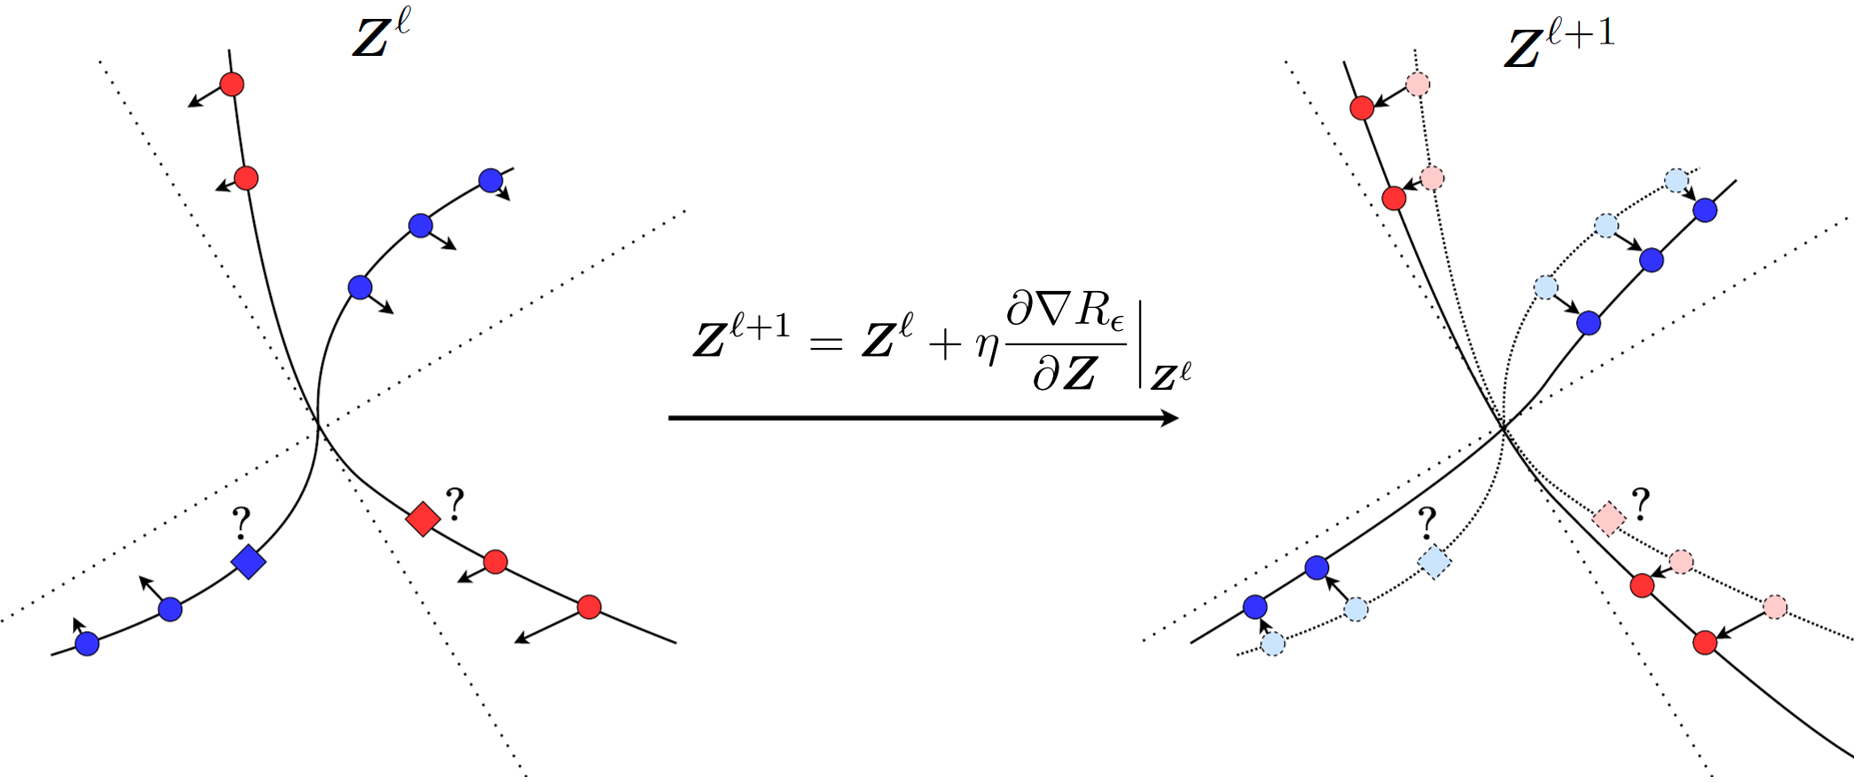
\includegraphics[width=0.85\linewidth]{\toplevelprefix/chapters/chapter4/figs/redu_gradient_diagram.png} 
    \caption{Deformare incrementală prin fluxul de gradient pentru a aplana atât datele din fiecare clasă într-un subspațiu și a împinge diferitele clase deoparte.} 
    \label{fig:gradient-flow}
\end{figure} 


Calculul simplu arată că gradientul ${\partial \Delta R_{\epsilon}}/{\partial \bm Z}$ implică evaluarea următoarelor derivate ale celor doi termeni din $\Delta R_{\epsilon}$:
\begin{equation}\label{eqn:expand-directions}
    \frac{1}{2}\frac{\partial \log \det (\I \!+\! \alpha \Z \Z^{\top} )}{\partial \bm Z}(\Z^\ell) = \underbrace{\alpha(\I \!+\! \alpha\Z^\ell (\Z^\ell)^\top)^{-1}}_{\bm E^{\ell} \; \in \Re^{d\times d}}\Z^\ell,
\end{equation}

\begin{equation}\label{eqn:compress-directions}
\frac{1}{2}\frac{\partial \left( \gamma_{k}  \log \det (\I + \alpha_{k} \Z \bm \Pi_k \Z^{\top} )  \right)}{\partial \bm Z}(\Z^\ell) = \gamma_{k}  \underbrace{ \alpha_{k}  (\I +  \alpha_{k} \Z^\ell \bm \Pi_k (\Z^\ell)^{\top})^{-1}}_{\bm C^{\ell}_k \; \in \Re^{d\times d}} \Z^{\ell} \bm \Pi_k.
\end{equation}
Observați că în cele de mai sus, matricea $\bm E^{\ell}$ depinde doar de $\Z^{\ell}$ și urmărește să {\em extindă} toate caracteristicile pentru a crește rata generală de codare; matricea $\bm C^{\ell}_{k}$ depinde de caracteristicile din clasa $k$ și urmărește să le {\em comprime} pentru a reduce rata de codare a fiecărei clase. 
Apoi gradientul complet $\frac{\partial \Delta R_{\epsilon}}{\partial \bm Z}(\Z^\ell) \in \Re^{d\times N}$ este de forma:
\begin{equation}
\frac{\partial \Delta R_{\epsilon}}{\partial \bm Z}(\Z^\ell)  = \underbrace{\bm E^{\ell}}_{\text{Expansiune}} \Z^{\ell} \;-\; \sum_{k=1}^K \gamma_{k} \underbrace{\bm C_{k}^{\ell}}_{\text{Compresie}}  \Z^{\ell} \bm{\Pi}_k.
\label{eqn:DR-gradient}
\end{equation}

\begin{remark}[Interpretarea $\bm E^\ell$ și $\bm C_j^\ell$ ca operatori liniari]\label{rem:regression-interpretation} 
Pentru orice $\bm z^\ell \in \mathbb{R}^d$,
\begin{gather}
    \bm E^\ell \bm z^\ell = \alpha(\bm z^\ell - \bm Z^\ell \bm q^\ell_\star), \qquad
    \mbox{unde} \qquad \bm q^\ell_\star \doteq \argmin_{\bm q^\ell} \big\{\alpha \|\bm z^\ell - \bm Z^\ell \bm q^\ell\|_2^2 + \|\bm q^\ell\|_2^2\big\}.
\end{gather}
Observați că $\bm q^\ell_\star$ este exact soluția regresiei ridge de către toate punctele de date $\bm Z^\ell$ în cauză. Prin urmare, $\bm E^\ell$ (similar pentru $\bm C^\ell_k$) este aproximativ (adică, când $N$ este suficient de mare) proiecția pe complementul ortogonal al subspațiului întins de coloanele lui $\bm Z^\ell$. Un alt mod de a interpreta matricea $\bm E^\ell$ este prin descompunerea în valori proprii a matricei de covarianță $\Z^\ell (\Z^\ell)^\top$. Presupunând că $\Z^\ell (\Z^\ell)^\top \doteq \bm U^\ell \bm \Lambda^\ell (\bm U^\ell)^\top$ unde $\bm \Lambda^\ell \doteq \diag\left(\lambda^\ell_1, \ldots, \lambda^\ell_d \right)$, avem 
\begin{equation}
\bm E^\ell = \alpha \bm U^\ell\, \diag\left(\frac{1}{1+\alpha\lambda^\ell_1}, \ldots, \frac{1}{1+\alpha\lambda^\ell_d}\right) \left(\bm U^\ell\right)^\top.
\end{equation}
Prin urmare, matricea $\bm E^\ell$ operează pe un vector $\bm z^\ell$ prin întindere într-un mod în care direcțiile de varianță mare sunt micșorate în timp ce direcțiile de varianță dispărută sunt păstrate. Acestea sunt exact direcțiile \eqref{eqn:expand-directions} în care mutăm caracteristicile astfel încât volumul general se extinde și rata de codare va crește, de aici semnul pozitiv. La efectul opus, direcțiile asociate cu \eqref{eqn:compress-directions} sunt „reziduuri" ale caracteristicilor fiecărei clase care deviază de la subspațiul căruia ar trebui să îi aparțină. Acestea sunt exact direcțiile în care caracteristicile trebuie să fie comprimate înapoi pe subspațiul lor respectiv, de aici semnul negativ (vezi \Cref{fig:regression-interpretation}). 

\begin{figure}[t]
    \centering
    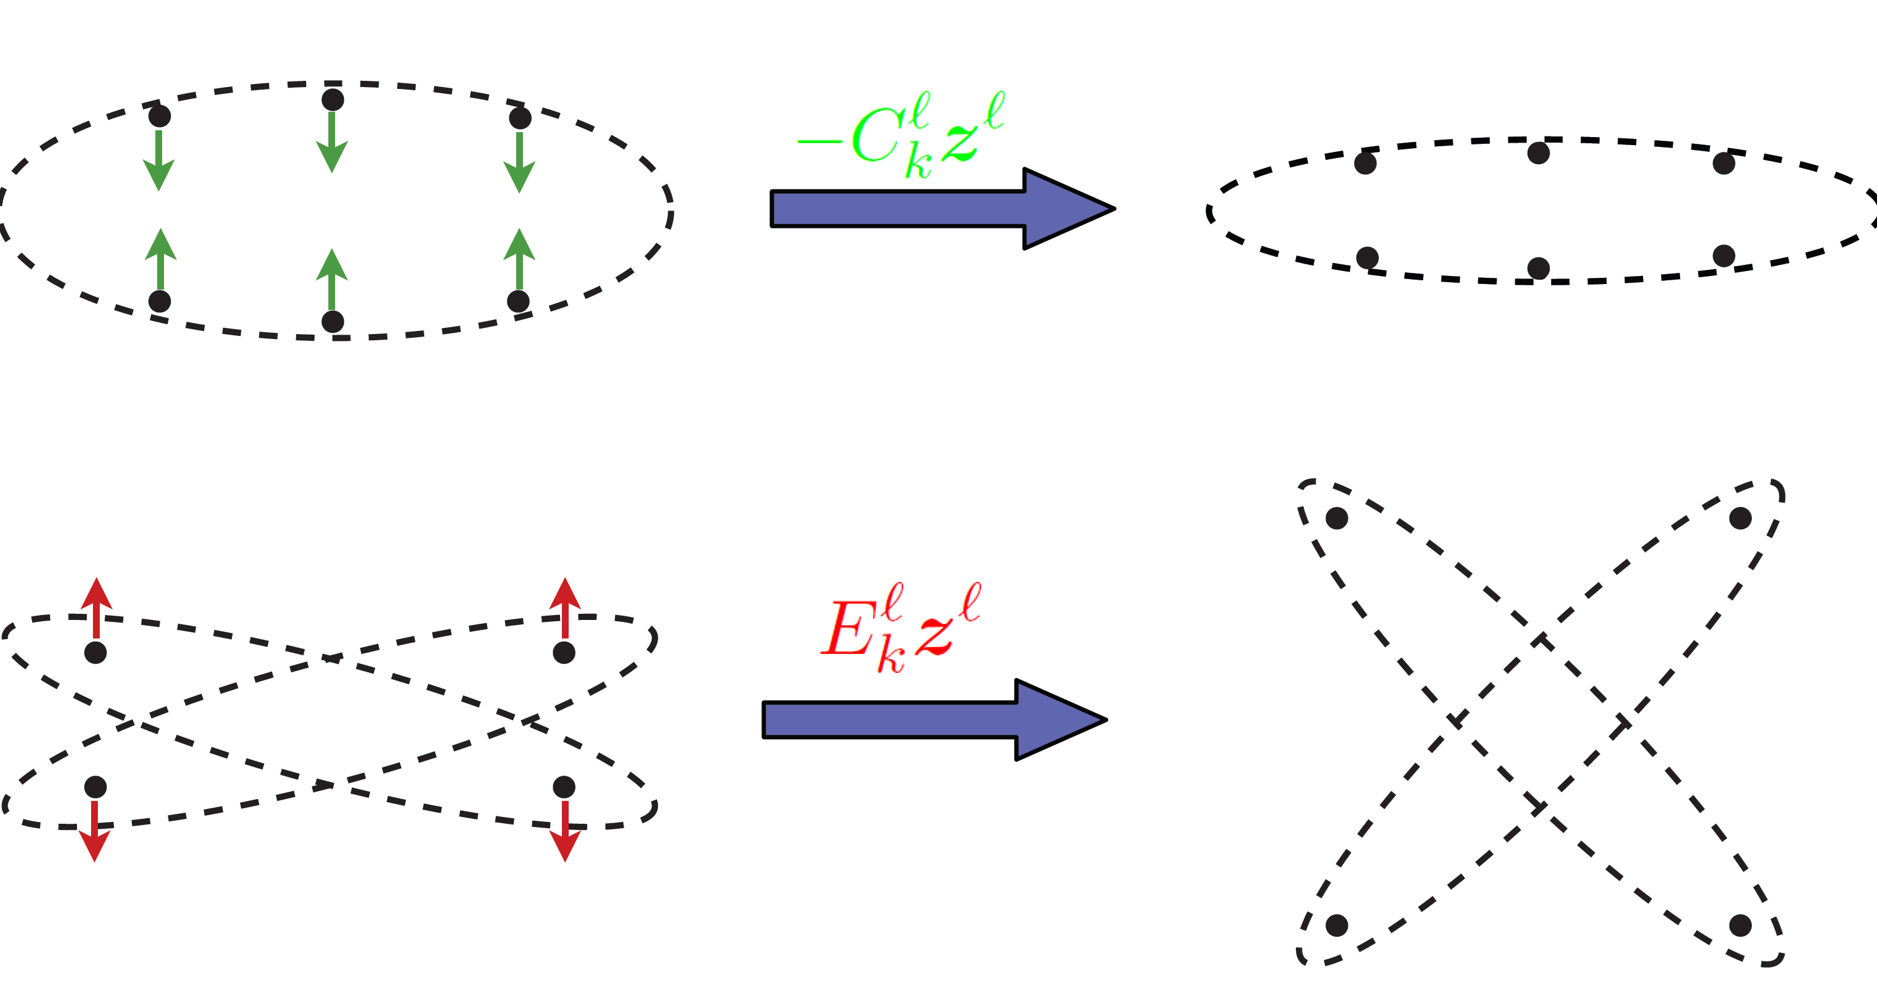
\includegraphics[width=0.65\linewidth]{\toplevelprefix/chapters/chapter4/figs/expand_compress.png}
    \caption{\small Interpretarea $\bm C^\ell_k$ și $\bm E^\ell$: $\bm C^\ell_k$ comprimă fiecare clasă prin contractarea caracteristicilor la un subspațiu de dimensiune redusă; $\bm E^\ell$ extinde toate caracteristicile prin contrastarea și respingerea caracteristicilor din diferite clase.}
    \label{fig:regression-interpretation}
    \vspace{-0.1in}
\end{figure}


În esență, operațiile liniare $\bm E^\ell$ și $\bm C_k^\ell$ în ascendența gradientului pentru reducerea ratei sunt determinate de datele de antrenament care efectuează „auto-regresii". Înțelegerea reînnoită recentă despre regresia ridge într-un cadru supra-parametrizat \cite{yang2020rethinking,Wu2020OnTO} indică faptul că utilizarea datelor aparent redundant eșantionate (din fiecare subspațiu) ca regresori nu duce la supraadaptare.
\end{remark}

\paragraph{Incrementul Hărții de Caracteristici Ghidat de Gradient.} Observați că în cele de mai sus, ascendența gradientului consideră toate caracteristicile $\Z^{\ell} = [\z^{\ell}_{1}, \dots, \z^{\ell}_{N}]$ ca variabile libere. Incrementul $\Z^{\ell+1} - \Z^{\ell} = \eta \frac{\partial \Delta R_{\epsilon}}{\partial \bm Z}(\Z^\ell)$ nu oferă încă o transformare pe întregul domeniu al caracteristicilor $\z^\ell \in \Re^d$. Conform ecuației \eqref{eqn:DR-gradient}, gradientul nu poate fi evaluat într-un punct a cărui apartenență nu este cunoscută, așa cum este ilustrat în \Cref{fig:gradient-flow}. Prin urmare, pentru a găsi $f(\x,\bm  \theta)$ optim în mod explicit, putem considera construirea unei transformări de increment mic $g(\cdot, \bm{\theta}^{\ell})$ pe caracteristica stratului $\ell$-lea $\z^\ell$ pentru a emula schema de gradient (proiectată) de mai sus:
\begin{equation}
\z^{\ell + 1}   \; \propto \; \z^{\ell} + \eta\cdot  g(\z^{\ell}, \bm{\theta}^{\ell}) \quad \mbox{cu condiția ca} \quad \z^{\ell +1} \in \mathbb{S}^{d-1}
\label{eqn:gradient-descent-transform}
\end{equation}
astfel încât $\big[g(\z_1^{\ell}, \bm \theta^{\ell}), \ldots, g(\z_N^{\ell}, \bm \theta^{\ell}) \big] \approx \frac{\partial \Delta R_{\epsilon}}{\partial \bm Z}(\Z^\ell).$ Adică, trebuie să aproximăm fluxul de gradient $\frac{\partial \Delta R_{\epsilon}}{\partial \bm Z}$ care deformează local toate caracteristicile (de antrenament) $\{\z_i^\ell\}_{i=1}^N$ cu o mapare continuă $g(\z,\bm \theta)$ definită pe întregul spațiu al caracteristicilor $\z^\ell \in \Re^d$.  
Observați că se poate interpreta incrementul \eqref{eqn:gradient-descent-transform} ca o versiune discretizată a unei ecuații diferențiale continue:
\begin{equation}
\dot{\z} = g(\z, \theta).
\end{equation}
Prin urmare, rețeaua (profundă) astfel construită poate fi interpretată ca o anumită ODE neuronală \cite{chen2018neural}. Cu toate acestea, spre deosebire de ODE neuronală unde fluxul $g$ este ales să fie unele structuri generice, aici $g(\z, \bm\theta)$ nostru este pentru a emula fluxul de gradient al reducerii ratei pe setul de caracteristici (așa cum se arată în \Cref{fig:gradient-flow}): 
\begin{equation*}
    \dot{\Z} = \frac{\partial \Delta R_{\epsilon}}{\partial \bm Z},
\end{equation*} 
și structura sa este în întregime derivată și complet determinată din acest obiectiv, fără alte priorități sau euristici.  

Prin inspecția structurii gradientului \eqref{eqn:DR-gradient}, sugerează că un candidat natural pentru transformarea de increment $g(\z^\ell, \bm \theta^\ell)$ este de forma:
\begin{equation}
    g(\z^\ell, \bm \theta^\ell) \; \doteq \; \bm E^\ell \z^\ell - \sum_{k=1}^K \gamma_{k} \pi_k(\z^\ell)\bm C_{k}^{\ell}  \z^{\ell}  \in \Re^d,
    \label{eqn:DR-gradient-transform}
\end{equation}
unde $\pi_k(\z^\ell) \in [0,1]$ indică probabilitatea ca $\z^{\ell}$ să aparțină clasei $k$-a. Parametrii hărții de increment $\bm \theta^\ell$ depind de: În primul rând, un set de hărți liniare reprezentate de $\bm E^{\ell}$ și $\{ \bm C^{\ell}_{k}\}_{k=1}^{K}$ care depind doar de statisticile caracteristicilor antrenamentului $\Z^\ell$; În al doilea rând, apartenența $\{ \pi_k(\z^\ell)\}_{k=1}^K$ a oricărei caracteristici $\z^\ell$. 
Observați că pe eșantioanele de antrenament $\Z^\ell$, pentru care apartenențele $\bm \Pi_k$ sunt cunoscute, $g(\z^\ell, \bm \theta)$ astfel definit oferă exact valorile pentru gradientul $\frac{\partial \Delta R_{\epsilon}}{\partial \bm Z}(\Z^\ell)$.  


Deoarece avem apartenența doar pentru eșantioanele de antrenament, funcția $g(\cdot)$ definită în \eqref{eqn:DR-gradient-transform} poate fi evaluată doar pe antrenament. Pentru a extrapola $g(\cdot)$ la întregul spațiu al caracteristicilor, trebuie să estimăm $\pi_k(\z^\ell)$ în al doilea său termen. În învățarea profundă convențională, această hartă este de obicei modelată ca o rețea profundă și învățată din datele de antrenament, să zicem prin {\em retropropagare}. Cu toate acestea, scopul nostru aici nu este să învățăm deja un clasificator precis $\pi_{k}(\z^\ell)$. În schimb, avem nevoie doar de o estimare suficient de bună a informațiilor clasei pentru ca $g(\cdot)$ să aproximeze bine gradientul $\frac{\partial \Delta R_{\epsilon}}{\partial \bm Z}$. 



Din interpretarea geometrică a hărților liniare $\bm E^\ell$ și $\bm C_k^\ell$ dată de \Cref{rem:regression-interpretation}, termenul $\bm p_{k}^{\ell} \doteq \bm C^{\ell}_k \z^{\ell}$ poate fi privit ca (aproximativ) proiecția lui $\z^{\ell}$ pe complementul ortogonal al fiecărei clase $j$. Prin urmare, $\|\bm p_{j}^{\ell}\|_2$ este mic dacă $\z^\ell$ este în clasa $j$ și mare în caz contrar. Aceasta ne motivează să estimăm apartenența sa pe baza următoarei funcții softmax:
\begin{equation}
    \widehat{\vpi}(\z^\ell) \doteq \softmax\rp{-\lambda\mat{\norm{\vC^{\ell}_{1}\vz^{\ell}}_{2} \\ \vdots \\ \norm{\vC^{\ell}_{K}\vz^{\ell}}_{2}}} = \frac{1}{\sum_{k = 1}^{K}\exp(-\lambda \norm{\vC^{\ell}_{k}\vz^{\ell}}_{2})}\mat{\exp(-\lambda\norm{\vC^{\ell}_{1}\vz^{\ell}}_{2}) \\ \vdots \\ \exp(-\lambda\norm{\vC^{\ell}_{K}\vz^{\ell}}_{2})} \in [0,1]^{K}.
\end{equation}
Prin urmare, al doilea termen al \eqref{eqn:DR-gradient-transform} poate fi aproximat de această apartenență estimată:
\begin{align}
\sum_{k=1}^K \gamma_{k} \pi_k(\z^\ell)\bm C_{k}^{\ell}  \z^{\ell} 
\; \approx \;  \sum_{k=1}^K \gamma_{k} \widehat{\pi}_k(\z^\ell)  \bm{C}^{\ell}_k  \z^{\ell} 
\; \doteq \; \bm \sigma\Big([\bm{C}^{\ell}_{1} \z^{\ell}, \dots, \bm{C}^{\ell}_{K} \z^{\ell}]\Big),
\label{eqn:soft-residual}
\end{align}
care este notată ca un operator neliniar $\bm \sigma(\cdot)$ pe ieșirile caracteristicii $\z^\ell$ prin $K$ grupuri de filtre: $[\bm{C}^{\ell}_{1}, \dots, \bm{C}^{\ell}_{K}]$. Observați că neliniaritatea apare datorită unei atribuiri „moi" a apartenenței la clasă pe baza răspunsurilor caracteristicilor de la aceste filtre.  

În general, combinând \eqref{eqn:gradient-descent-transform}, \eqref{eqn:DR-gradient-transform}, și \eqref{eqn:soft-residual}, 
transformarea caracteristicii de increment de la $\z^{\ell}$ la $\z^{\ell+1}$ devine acum
\begin{equation}\label{eqn:layer-approximate}
\begin{aligned}
\z^{\ell+1}  &\propto \; \z^\ell +  \eta \cdot  \bm E^{\ell} \z^{\ell} - \eta\cdot  \bm \sigma\big([\bm{C}^{\ell}_{1} \z^{\ell}, \dots, \bm{C}^{\ell}_{K} \z^{\ell}]\big)  \\
&= \; \z^\ell +  \eta \cdot g(\z^\ell, \bm \theta^\ell) \qquad \mbox{cu condiția ca} \quad \z^{\ell +1} \in \mathbb{S}^{d-1},
\end{aligned}
\end{equation}
cu funcția neliniară $\bm \sigma(\cdot)$ definită mai sus și $\bm \theta^\ell$ colectând toți parametrii pe straturi. Adică $\bm \theta^\ell =\left\{\bm E^\ell, \bm{C}^{\ell}_{1}, \dots, \bm{C}^{\ell}_{K}, \gamma_{k}, \lambda\right\}$. Notați că caracteristicile la fiecare strat sunt întotdeauna „normalizate" prin proiectarea pe sfera unitară $\mathbb S^{d-1}$, notată ca $\mathcal P_{\mathbb S^{d-1}}$. Forma incrementului în \eqref{eqn:layer-approximate} poate fi ilustrată printr-o diagramă în \Cref{fig:arch-ReduNet}(a).

\begin{figure}[t]
    \begin{subfigure}[t]{0.35\textwidth}
        \centering
        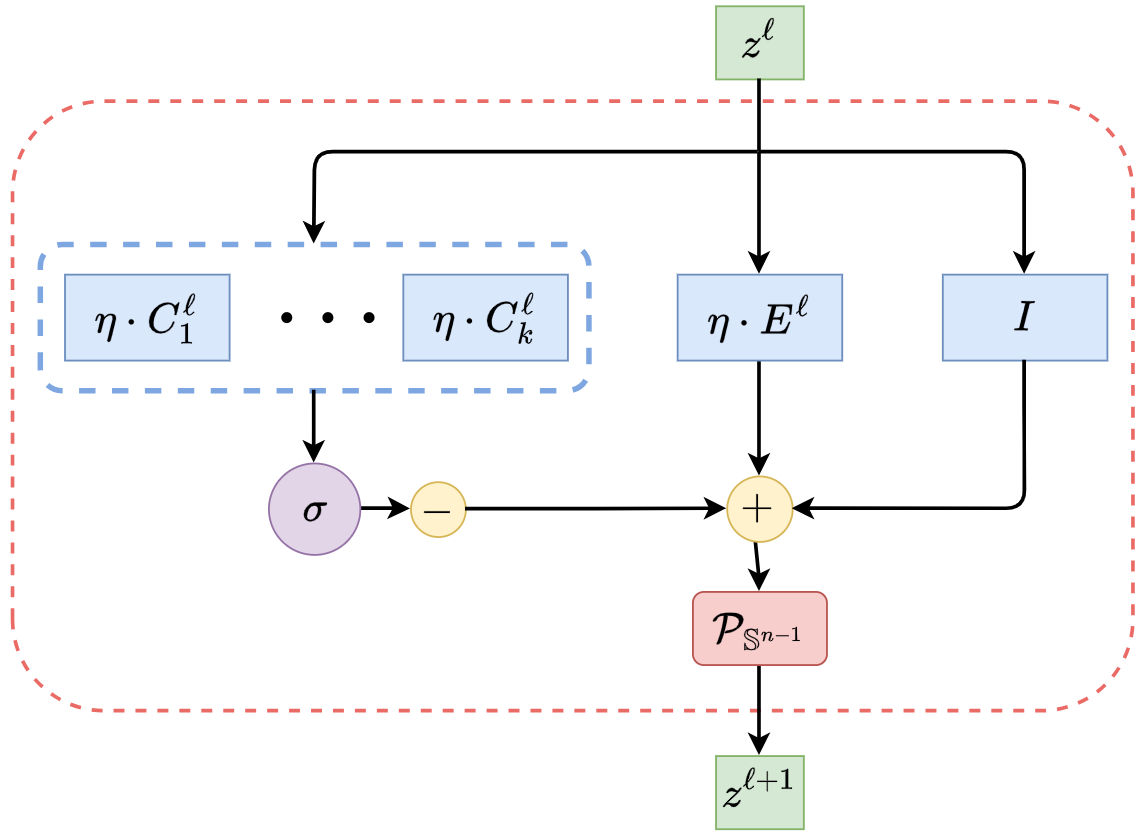
\includegraphics[width=\textwidth]{\toplevelprefix/chapters/chapter4/figs/redunet_layer.png}
        \caption{\textbf{ReduNet}}
    \end{subfigure}
    \hfill 
    \begin{subfigure}[t]{0.6\textwidth}
        \centering
        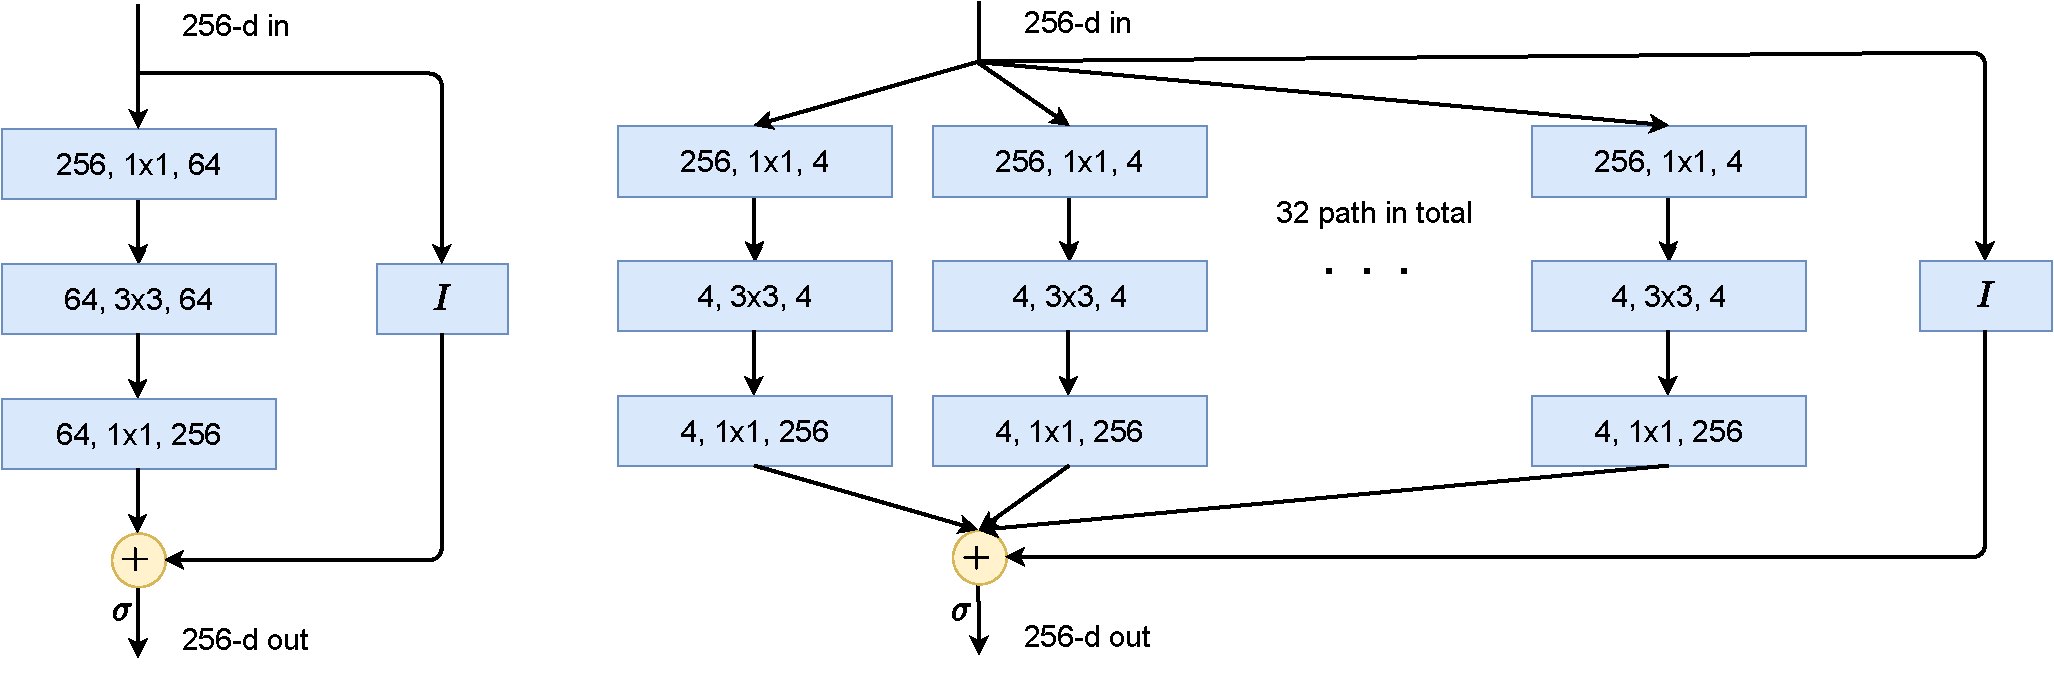
\includegraphics[width=\textwidth]{\toplevelprefix/chapters/chapter4/figs/resnet_resnext.pdf}
        \caption{\textbf{ResNet} și \textbf{ResNeXt}.}
    \end{subfigure}
    \caption{\small Arhitecturi de rețea ale ReduNet și comparație cu altele. \textbf{(a)}: Structura stratului \textbf{ReduNet} derivată dintr-o iterație de ascendență gradient pentru optimizarea reducerii ratei. \textbf{(b)} (stânga): Un strat de ResNet~\cite{he2016deep}; și \textbf{(b)} (dreapta): Un strat de ResNeXt~\cite{ResNEXT}. După cum vom vedea în \Cref{sec:shift-invariant}, operatorii liniari $\bm E^\ell$ și $\bm{C}_k^\ell$ ai ReduNet devin în mod natural convoluții (multi-canal) când se impune invarianța la deplasare.}
    \label{fig:arch-ReduNet}
\end{figure}

\begin{algorithm}[t]
    \caption{Algoritm de antrenament pentru ReduNet}
    \label{alg:redunet_training}
    \begin{algorithmic}[1]
        \Require{$\vX = [\vx_1, \ldots, \vx_N]\in \Re^{D \times N}$, $\bm{\Pi} = \{\bm \Pi_k\}_{k=1}^K$, $\epsilon > 0$, $\lambda$, și o rată de învățare $\eta$.}
        \Ensure{Parametrii învățați \(\{\vE^{\ell}\}_{\ell = 1}^{L}, \{\{\vC^{\ell}_{k}\}_{k = 1}^{K}\}_{\ell = 1}^{L}, \{\gamma_{k}\}_{k = 1}^{k}\)}

        \Procedure{ReduNetTraining}{$\vX, \vPi, \epsilon, \lambda, \eta$}
            \Statex{\quad\ \texttt{\# Definirea constantelor}}

            \State{\(\alpha \gets d/(N\epsilon^{2})\)}
            \For{\(k \in \{1, \dots, K\}\)}
            \State{\(\alpha_{k} \gets D/(\tr(\vPi_{k})\epsilon^{2})\)}
            \State{\(\gamma_{k} \gets \tr(\vPi_{k})/D\)}
            \EndFor
            \Statex{}

            \Statex{\quad\ \texttt{\# Iterația strat cu strat ReduNet}}
            \State{\(\vZ^{1} = \mat{\vz_{1}^1, \dots, \vz_{N}^1} \gets \vX\)} \Comment{Inițializează iterația pe strat ReduNet}
            \For{\(\ell \in \{1, \dots, L\}\)}
                \Statex{\quad\ \texttt{\# Pasul 1: Calculează parametrii rețelei} \(\vE^{\ell}, \{\vC^{\ell}_{k}\}_{k = 1}^{K}\)}
                \State{\(\vE^{\ell} \gets \alpha\left(\vI + \alpha \vZ^{\ell}(\vZ^{\ell})^{\top}\right)^{-1} \in \R^{d \times d}\)}
                \For{\(k \in \{1, \dots, K\}\)}
                    \State{\(\vC^{\ell}_{k} \gets \alpha_{k}\left(\vI + \alpha_{k}\vZ^{\ell}\vPi_{k}(\vZ^{\ell})^{\top}\right)^{-1} \in \R^{d \times d}\)}
                \EndFor
                \Statex{}
                \Statex{\qquad\quad\texttt{\# Pasul 2: Actualizează caracteristicile \(\vZ^{\ell}\)}}
                \For{\(i \in \{1, \dots, N\}\)}
                    \State{\(\hat{\vpi}(\vz^{\ell}_i) \gets \displaystyle \softmax(-\lambda[\norm{\vC^{\ell}_{1}\vz^{\ell}_i}_{2}, \dots, \norm{\vC^{\ell}_{K}\vz^{\ell}_i}_{2}]) \in [0, 1]^{K}\)} \Comment{Calculează atribuirile moi \(\hat{\vpi}(\vz^{\ell}_i)\)}
                    \State{\(\displaystyle\vz^{\ell + 1}_i \gets \cP_{\bS^{d - 1}}\rp{\vz^{\ell}_i + \eta \bp{\vE^{\ell}\vz^{\ell}_i - \sum_{k = 1}^{K}\gamma_{k}\hat{\pi}_{k}(\vz^{\ell}_i) \vC^{\ell}_{k}\vz^{\ell}_i}} \in \R^{d}\)} \Comment{Actualizează caracteristicile \(\vz^{\ell + 1}_i\) din \(\vz^{\ell}_i\)}
                \EndFor
            \EndFor
            \State{\Return{\(\{\vE^{\ell}\}_{\ell = 1}^{L}, \{\{\vC^{\ell}_{k}\}_{k = 1}^{K}\}_{\ell = 1}^{L}, \{\gamma_{k}\}_{k = 1}^{K}\)}} \Comment{Returnează toți parametrii rețelei.}
        \EndProcedure
    \end{algorithmic}
\end{algorithm}


\paragraph{Rețea Profundă pentru Optimizarea Reducerii Ratei.} Observați că incrementul este construit pentru a emula ascendența gradientului pentru reducerea ratei $\Delta R_\epsilon$. Prin urmare, prin transformarea caracteristicilor iterativ prin procesul de mai sus, ne așteptăm ca reducerea ratei să crească, așa cum vom vedea în secțiunea experimentală. Acest proces iterativ, odată conversat să zicem după $L$ iterații, oferă harta de caracteristici dorită $f(\x, \bm \theta)$ pe intrarea $\x = \z^0$, exact în forma unei {\em rețele profunde}, în care fiecare strat are structura prezentată în \Cref{fig:arch-ReduNet} stânga:
\begin{equation}\label{eqn:ReduNet}
\begin{aligned}
f(\x, \bm \theta)\; =&  \;\;f^L \circ f^{L-1} \circ  \cdots \circ f^1 \circ
    f^0(\z^0),  \\ 
f^\ell(\z^\ell, \bm \theta^\ell) \; \doteq & \;\; \z^{\ell+1} = \mathcal{P}_{\mathbb{S}^{n-1}}[\z^{\ell} + \eta\cdot g(\z^{\ell}, \bm \theta^{\ell})], \\
g(\z^{\ell}, \bm \theta^{\ell}) \; =&\;\; \bm E^{\ell} \z^{\ell} -  \bm \sigma\big([\bm{C}^{\ell}_{1} \z^{\ell}, \dots, \bm{C}^{\ell}_{K} \z^{\ell}]\big).
\end{aligned}
\end{equation}
Deoarece această rețea profundă este derivată din maximizarea \textbf{redu}cerii ratei, o numim \textbf{ReduNet}. Comparând arhitectura ReduNet cu cele ale rețelelor populare proiectate empiric, \textbf{ResNet} și \textbf{ResNeXt} prezentate în \Cref{fig:arch-ReduNet}, similitudinea este oarecum uimitoare. Conceptual, ReduNet ar putea fi folosit și pentru a justifica arhitectura populară mixtură de experți (\textbf{MoE}) \cite{MoE} deoarece fiecare canal paralel, $\bm{C}^{\ell}_k$, poate fi privit ca un „expert" antrenat pentru fiecare clasă de obiecte.

\begin{figure}[t]
    \centering
    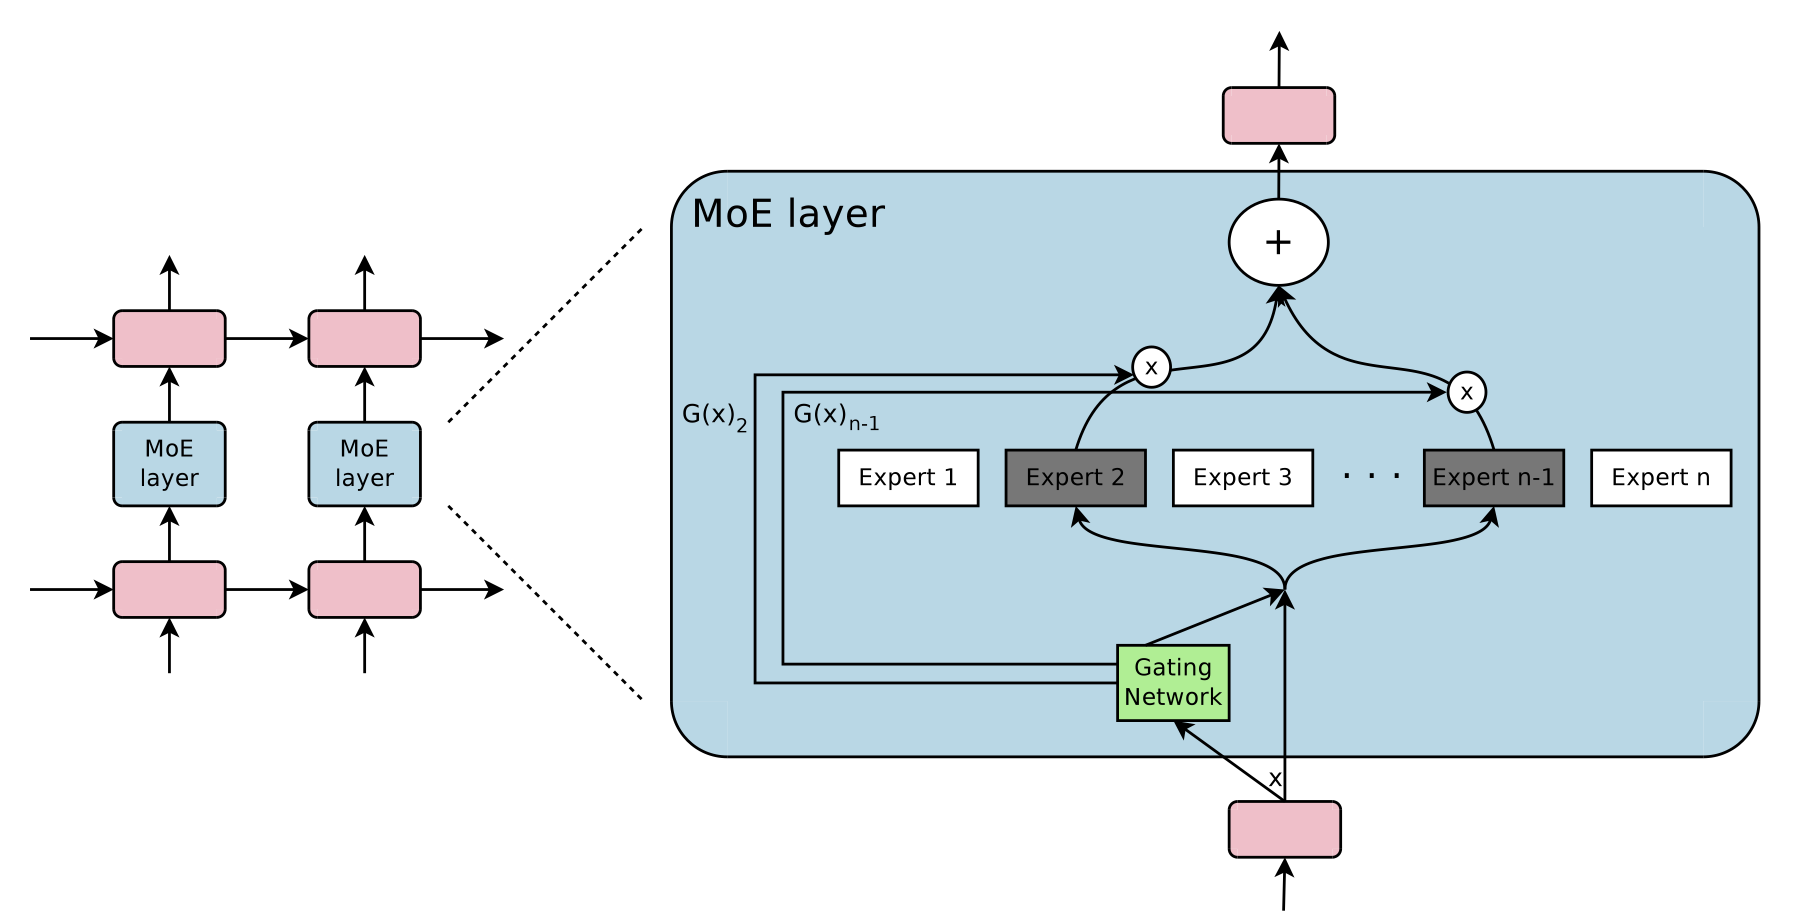
\includegraphics[width=0.45\linewidth]{\toplevelprefix/chapters/chapter4/figs/MoE.png} \hspace{5mm}
    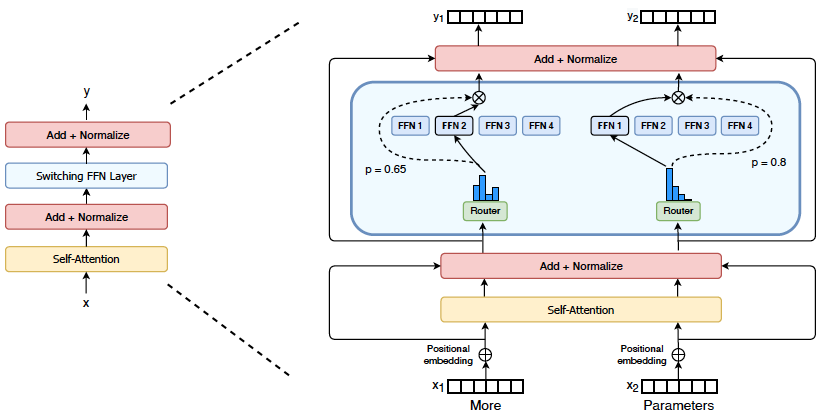
\includegraphics[width=0.45\linewidth]{\toplevelprefix/chapters/chapter4/figs/switched-transformer.png}
    \caption{Stânga: o rețea profundă mixtură de experți (MoE) \cite{MoE}. Dreapta: un Switch Transformer care promovează sparsitatea \cite{Fedus-2022}, folosit pentru a implementa MoE cu 1,7 trilioane de parametri.}
    \label{fig:enter-label}
\end{figure}

Rezumăm antrenamentul și evaluarea ReduNet în \Cref{alg:redunet_training} și \Cref{alg:redunet_evaluation}, respectiv. Observați că toți parametrii rețelei sunt construiți explicit strat cu strat într-o manieră de {\em propagare înainte}. Construcția nu are nevoie de nicio retropropagare! Caracteristicile astfel învățate pot fi folosite direct pentru clasificare, să zicem printr-un clasificator de cel mai apropiat subspațiu. 



\begin{algorithm}[!htbp]
    \caption{Algoritm de evaluare pentru ReduNet}
    \label{alg:redunet_evaluation}
    \begin{algorithmic}[1]
        \Require{Intrare \(\vx \in \R^{D}\), parametrii rețelei \(\{\vE^{\ell}\}_{\ell = 1}^{L}, \{\{\vC^{\ell}_{k}\}_{k = 1}^{K}\}_{\ell = 1}^{L}, \{\gamma_{k}\}_{k = 1}^{K}\), rata de învățare \(\lambda\)}
        \Ensure{caracteristica \(\vz^{L + 1}\)}

        \Procedure{ReduNetEvaluation}{$\vx$}
        \State{\(\vz^{1} \gets \vx \in \R^{D}\)} \Comment{Inițializează iterația pe strat ReduNet}
        \For{\(\ell \in \{1, \dots, L\}\)}
        \State{\(\hat{\vpi}(\vz^{\ell}) \gets  \softmax(-\lambda\mat{\norm{\vC^{\ell}_{1}\vz^{\ell}}_{2}, \dots, \norm{\vC^{\ell}_{K}\vz^{\ell}}_{2}}) \in [0, 1]^{K}\)} \Comment{Calculează atribuirile moi \(\hat{\vpi}(\vz^{\ell})\)}
        \State{\(\vz^{\ell + 1} \gets \cP_{\bS^{d - 1}}\rp{\vz^{\ell} + \eta \bp{\vE^{\ell}\vz^{\ell} - \sum_{k = 1}^{K}\gamma_{k}\hat{\pi}_{k}(\vz^{\ell}) \vC^{\ell}_{k}\vz^{\ell}}} \in \R^{d}\)} \Comment{Actualizează caracteristica \(\vz^{\ell + 1}\) folosind \(\vz^{\ell}\)}
        \EndFor
        \State{\Return{\(\vz^{L + 1}\)}} \Comment{Returnează caracteristicile de ieșire}
        \EndProcedure
    \end{algorithmic}
\end{algorithm}


\begin{example}
Pentru a oferi o intuiție despre cum ReduNet transformă caracteristicile, oferim un exemplu simplu cu Gaussiene 3D amestecate și vizualizăm cum sunt transformate caracteristicile în \Cref{fig:redu-3d-gaussian-diagram}. 
Considerăm un amestec de trei distribuții Gaussiene în $\R^{3}$ care este proiectat pe $\mathbb{S}^2$. Mai întâi generăm puncte de date pentru 3 clase: pentru $k=1,2,3$, $\bm{X}_{k}=[\bm{x}_{k,1}, \ldots, \bm{x}_{k,m}] \in \R^{3\times m}$, $\bm{x}_{k,i} \sim \mathcal{N}(\bm{\mu}_{k}, \sigma_{k}^{2} \I)$, și ${\pi}(\x_{k,i}) = k$.
Setăm $m=500, \sigma_{1}=\sigma_{2}=\sigma_{3}=0.1$, și $\bm{\mu}_{1}, \bm{\mu}_{2}, \bm{\mu}_{3} \in \mathbb{S}^2$. 
Apoi proiectăm toate punctele de date pe $\mathbb{S}^{2}$, adică $\bm{x}_{k,i}/\|\bm{x}_{k,i}\|_{2}$. 
Pentru a construi rețeaua (calculând $\bm{E}^{\ell}, \bm{C}^{\ell}_{k}$ pentru stratul $\ell$-lea), setăm numărul de iterații/straturi $L=2.000$, dimensiunea pasului $\eta=0.5$, și precizia $\epsilon=0.1$. 
Facem aceasta doar pentru a demonstra că cadrul nostru duce la rețele profunde stabile chiar și cu mii de straturi. 
În practică, mii de straturi ar putea să nu fie necesare și se poate opri ori de câte ori adăugarea de noi straturi oferă randamente în scădere. 
Pentru acest exemplu, câteva sute de straturi sunt suficiente. Prin urmare, obiectivul clar de optimizare oferă un criteriu natural pentru adâncimea rețelei necesare.

După cum se arată în \Cref{fig:redu-3d-gaussian-diagram}, putem observa că după maparea $f(\cdot, \bm{\theta})$, eșantioanele din aceeași clasă sunt foarte comprimate și converg la un singur cluster și unghiul dintre două clustere diferite este aproximativ $\pi/2$, care este bine aliniat cu soluția optimă $\Z^{\star}$ a pierderii MCR$^2$ în $\mathbb{S}^2$. 
Pierderea MCR$^2$ a caracteristicilor pe diferite straturi poate fi găsită în \Cref{fig:redu-3d-gaussian-diagram}(\textbf{c}). Empiric, constatăm că ReduNet-ul construit este capabil să maximizeze pierderea MCR$^2$ și converge stabil și eșantioanele din aceeași clasă converg la un cluster și clusterele diferite sunt ortogonale unul față de celălalt. 
Mai mult, când eșantionăm noi puncte de date din aceleași distribuții, constatăm că noile eșantioane din aceeași clasă converg în mod consistent la același centru de cluster ca și eșantioanele de antrenament. 
\begin{figure}[t]
    \begin{subfigure}[t]{0.32\textwidth}
        \centering 
        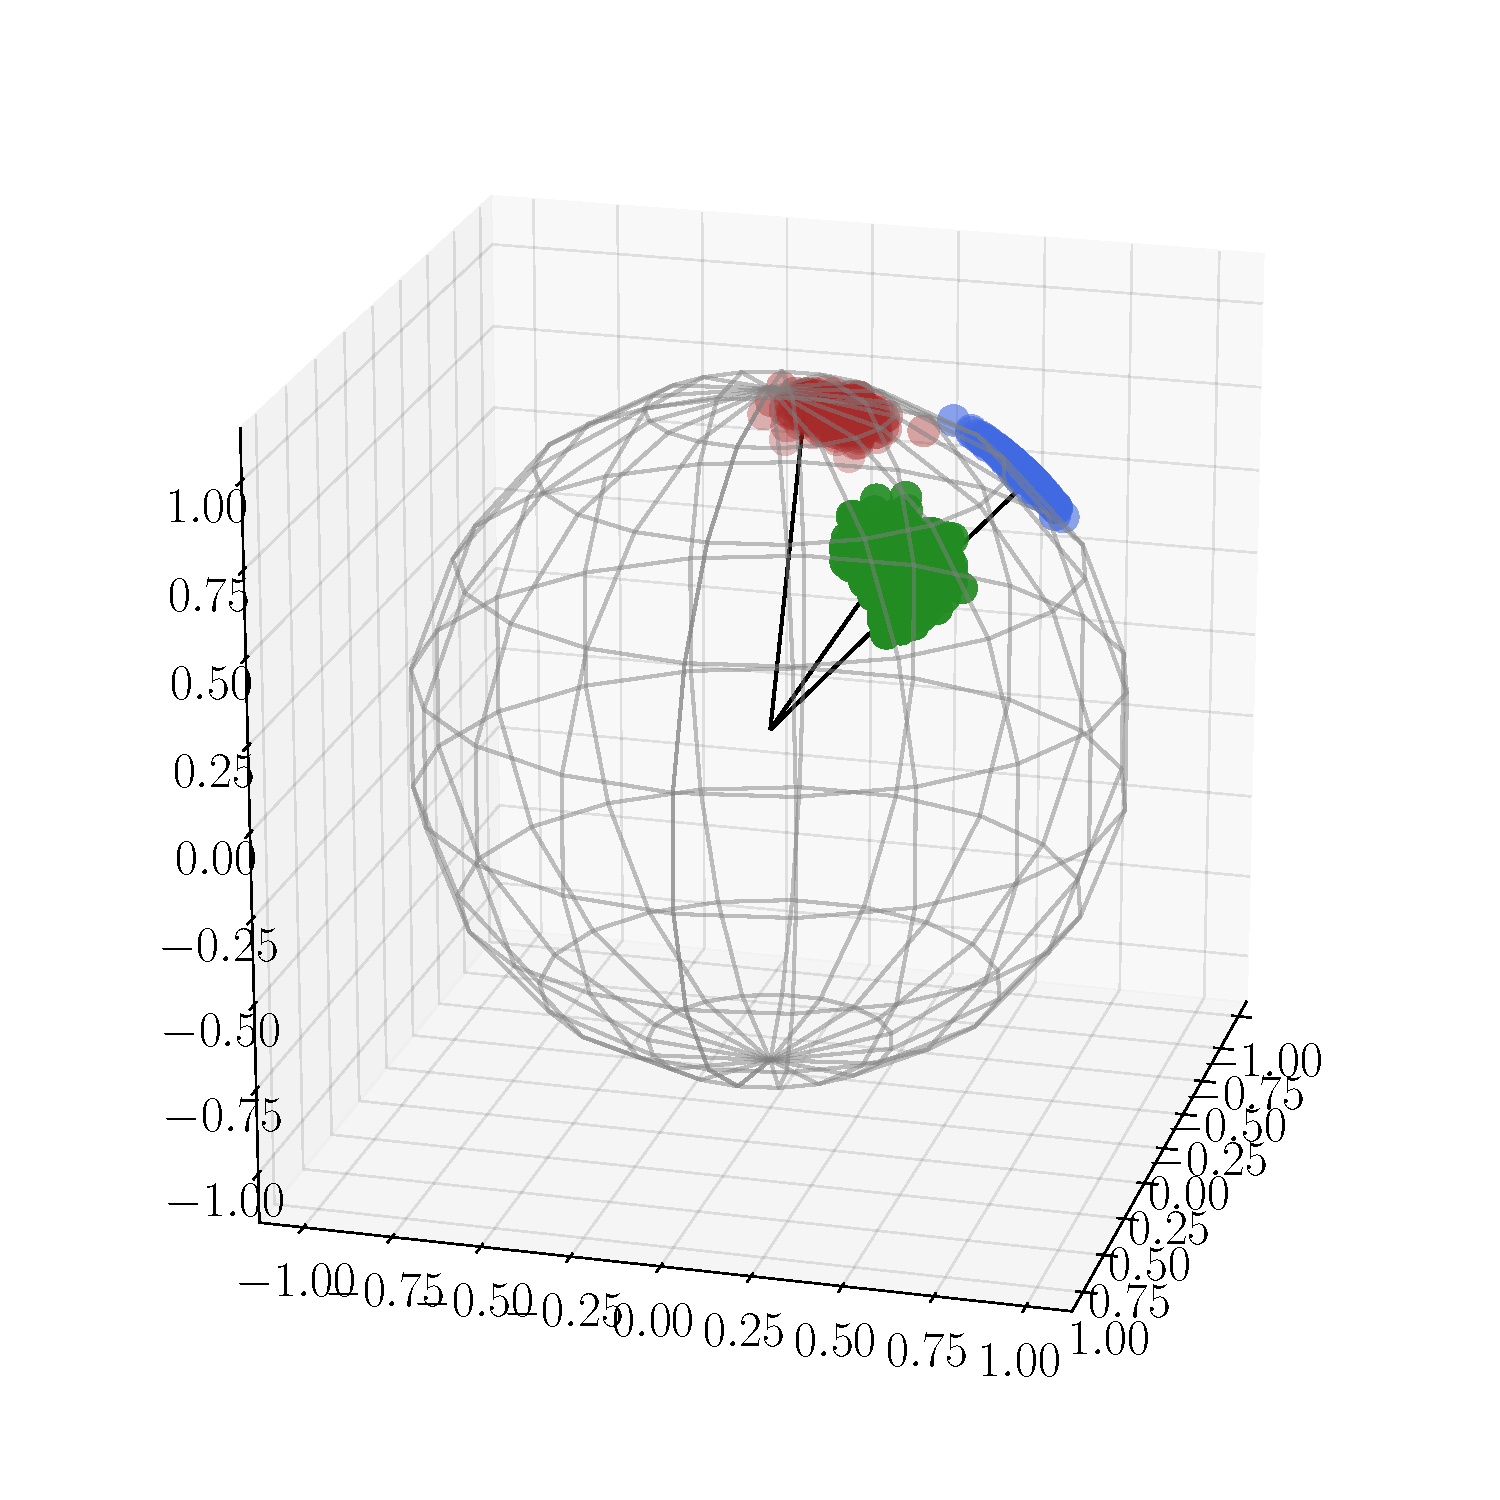
\includegraphics[width=\textwidth]{\toplevelprefix/chapters/chapter4/figs/scatter3d-X_train.pdf}\vspace{-0.1in}
        \caption{$\bm{X}_{\text{antrenament}}$}
    \end{subfigure}
    \hfill
    \begin{subfigure}[t]{0.32\textwidth}
        \centering 
        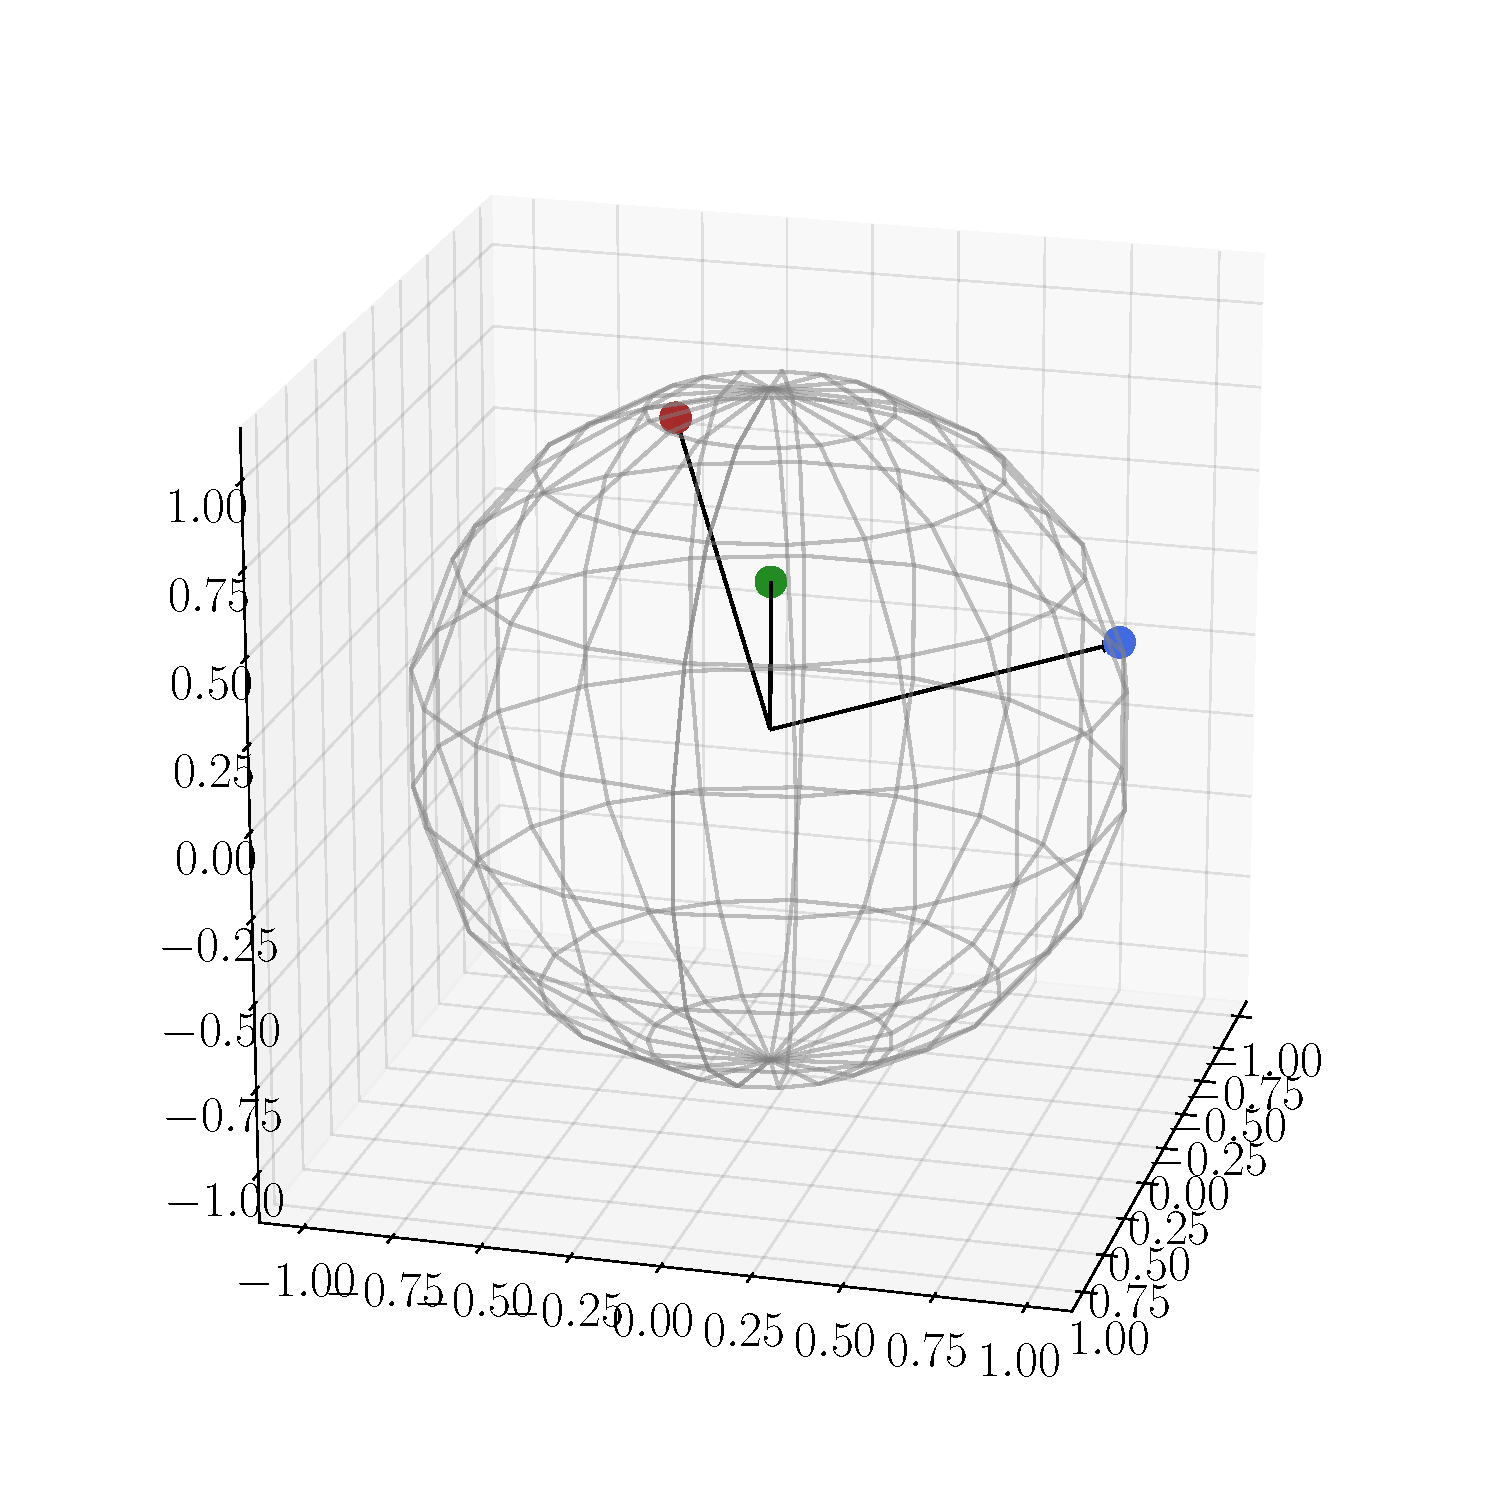
\includegraphics[width=\textwidth]{\toplevelprefix/chapters/chapter4/figs/scatter3d-Z_train.pdf}\vspace{-0.1in}
        \caption{$\bm{Z}_{\text{antrenament}}$}
    \end{subfigure}
    \hfill
    \begin{subfigure}[t]{0.32\textwidth}
        \centering 
        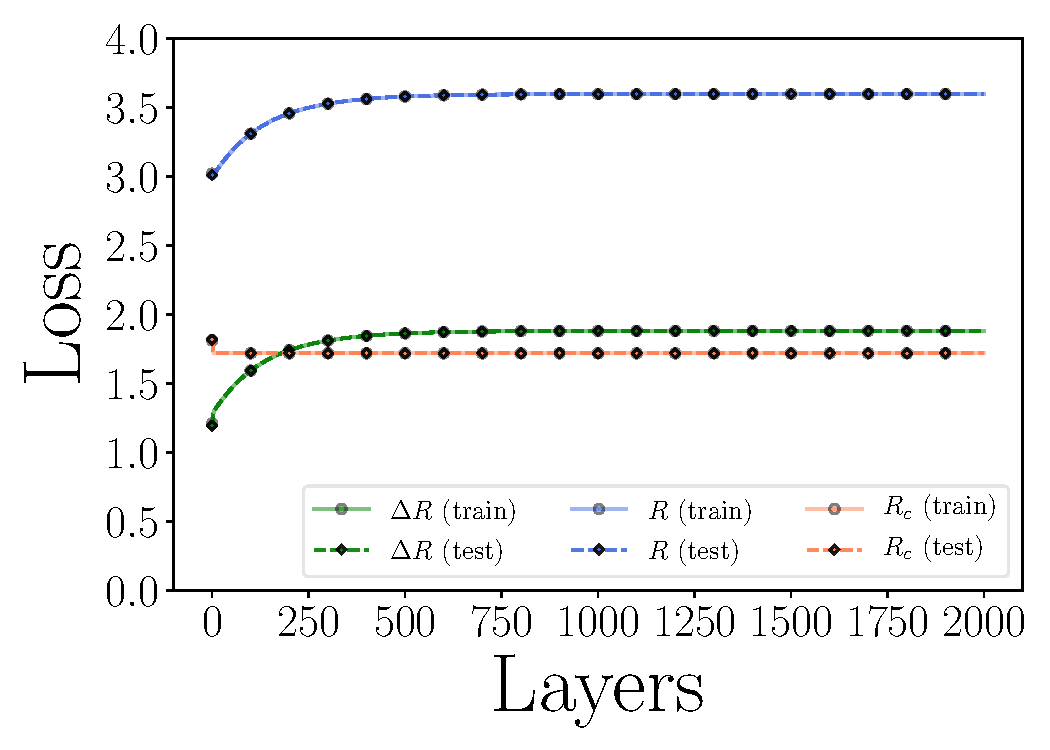
\includegraphics[width=\textwidth]{\toplevelprefix/chapters/chapter4/figs/scatter3d-loss-traintest.pdf}\vspace{-0.1in}
        \caption{Pierdere (antrenament/validare)}
    \end{subfigure}
    \vspace{-0.1in}
    \caption{\small Eșantioane originale și reprezentări învățate pentru Amestec de Gaussiene 3D. Vizualizăm punctele de date $\bm{X}$ (înainte de maparea $f(\cdot, \bm{\theta})$) în (\textbf{a}) și caracteristicile învățate $\bm{Z}$ (după maparea $f(\cdot, \bm{\theta})$) în (\textbf{b}) prin grafic de dispersie. În fiecare grafic de dispersie, fiecare culoare reprezintă o clasă de eșantioane. În (\textbf{c}), arătăm și graficele pentru progresia valorilor funcțiilor obiectiv.}
    \label{fig:redu-3d-gaussian-diagram}
\end{figure}

\end{example}

\subsection{Rețele Convoluționale din Reducerea Ratei Invariante}\label{sec:shift-invariant}

În secțiunea anterioară, am derivat arhitectura pe straturi a unei rețele profunde, ReduNet, folosind optimizarea desfășurată pentru obiectivul de reducere a ratei. 
În mod specific, termenul de compresie $R^c_\epsilon(\Z \mid\bm \Pi)$ în \eqref{eq:mcr-formulation} este proiectat pentru a comprima reprezentările din aceeași clasă. Cu toate acestea, această formulare nu ia în considerare posibila transformare sau deformare a domeniului datelor de intrare. De exemplu, deplasarea unui obiect ușor spre dreapta nu schimbă eticheta semantică a unei imagini. În această secțiune, vom demonstra cum straturile convoluționale pot fi derivate prin maximizarea unui obiectiv de reducere a ratei care este invariant la anumite deformări de domeniu, cum ar fi rotațiile și translațiile imaginilor. 


Pentru multe sarcini de clustering sau clasificare (cum ar fi detectarea obiectelor în imagini), considerăm două eșantioane ca fiind {\em echivalente} dacă diferă prin anumite clase de deformări sau augmentări de domeniu $\cT = \{\tau \}$. Prin urmare, suntem interesați doar de structuri de dimensiune redusă care sunt {\em invariante} la astfel de deformări~(adică, $\x \in \mathcal{M}$ dacă și numai dacă $\tau(\x) \in \mathcal{M}$ pentru toate $\tau \in \cT$\,), 
care sunt cunoscute a avea structuri geometrice și topologice sofisticate și pot fi dificil de învățat precis în practică, chiar și cu CNN-uri riguros proiectate \cite{Cohen-ICML-2016}. 
În acest cadru, aceasta poate fi formulată într-un mod foarte natural: toate instanțele echivariante trebuie să fie înglobate în același subspațiu, astfel încât subspațiul în sine să fie invariant la transformările luate în considerare.

În multe aplicații, cum ar fi datele seriale sau datele de imagini, semnificația semantică (etichetele) datelor sunt {\em invariante} la anumite transformări $\mathfrak{g} \in \mathbb{G}$ (pentru un anumit grup $\mathbb{G}$) \cite{CohenW16,deep-sets-NIPS2017}. De exemplu, semnificația unui semnal audio este invariantă la deplasarea în timp; și identitatea unui obiect într-o imagine este invariantă la translația în planul imaginii. Prin urmare, preferăm ca maparea caracteristicilor $f(\x,\bm \theta)$ să fie riguros invariantă la astfel de transformări:
\begin{equation}
\mbox{\em Invarianță de Grup:}\;   f(\x\circ \mathfrak{g}, \bm \theta) \sim f(\x,\bm \theta),\ \forall \mathfrak{g} \in \mathbb{G},
\end{equation}
unde „$\sim$" indică două caracteristici aparținând aceleiași clase echivalente. Deși pentru a asigura invarianța sau echivariența, operatorii convoluționali au fost o practică comună în rețelele profunde \cite{CohenW16}, rămâne dificil în practică să antrenezi o rețea de convoluție (proiectată empiric) de la zero care poate {\em garanta} invarianța chiar și la transformări simple precum translația și rotația \cite{azulay2018deep,engstrom2017rotation}. O abordare alternativă este să proiectezi cu atenție filtrele de convoluție ale fiecărui strat pentru a asigura invarianța translațională pentru o gamă largă de semnale, să zicem folosind wavelets ca în ScatteringNet \cite{scattering-net} și lucrări ulterioare \cite{Wiatowski-2018}. Cu toate acestea, pentru a asigura invarianța la semnale generice, numărul de convoluții necesare crește de obicei exponențial cu adâncimea rețelei. Acesta este motivul pentru care acest tip de rețea nu poate fi construit atât de profund, de obicei doar câteva straturi. 

Acum, arătăm că principiul MCR$^2$ este compatibil cu invarianța într-un mod natural și precis: trebuie doar să atribuim toate versiunile transformate $\{\x\circ \mathfrak{g} \mid \mathfrak{g} \in \mathbb G\}$ în aceeași clasă ca datele $\x$ și să mapăm caracteristicile lor $\z$ toate în același subspațiu $\mathcal S$. Prin urmare, toate informațiile echivariante de grup sunt codificate doar în interiorul subspațiului, și orice clasificator definit pe setul rezultat de subspații va fi automat invariant la astfel de transformări de grup. Vezi \Cref{fig:ortho-invariance-diagram} pentru o ilustrare a exemplelor de rotație 1D și translație 2D. În continuare, vom arăta riguros că atunci când grupul $\mathbb G$ este deplasarea circulară 1D, rețeaua profundă rezultată devine în mod natural o {\em rețea de convoluție multi-canal}. 
Deoarece rețeaua astfel construită trebuie să asigure invarianța doar pentru datele date $\X$ sau caracteristicile lor $\Z$, numărul de convoluții necesare rămâne de fapt constant printr-o rețea foarte profundă, spre deosebire de ScatteringNet. 

\begin{figure}[t]
    \begin{subfigure}[t]{0.4\textwidth}
        \centering 
        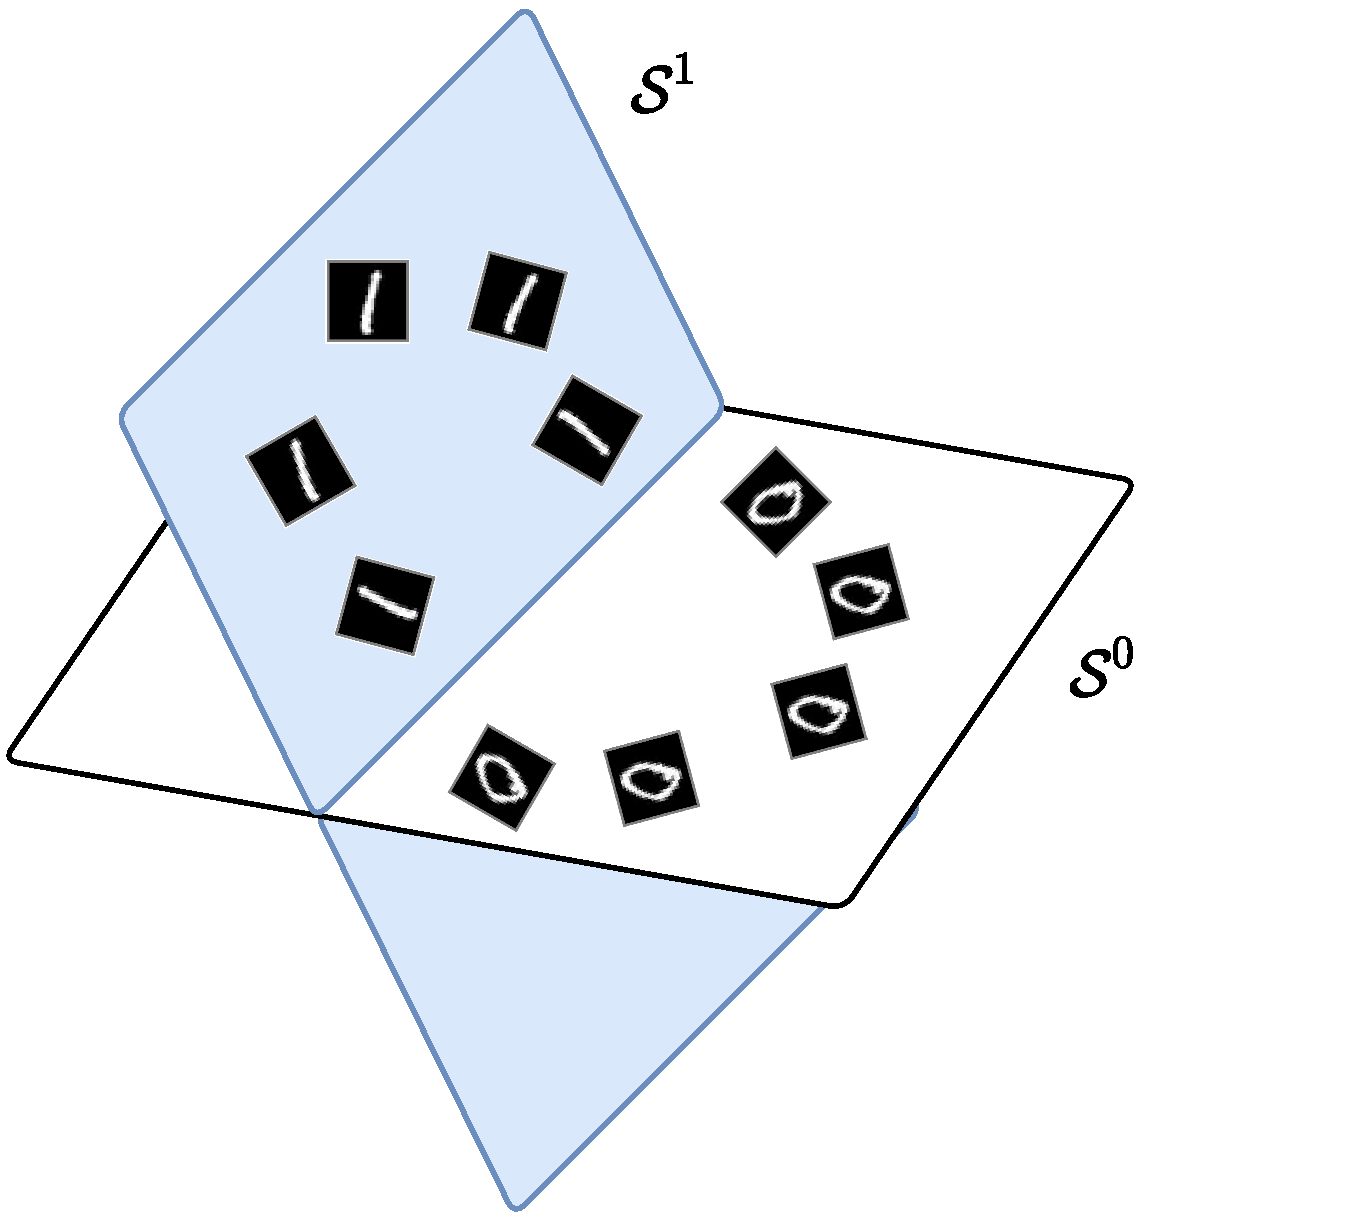
\includegraphics[width=\textwidth]{\toplevelprefix/chapters/chapter4/figs/ortho_diagram_1d.pdf}
    \end{subfigure}
    \hfill 
    \begin{subfigure}[t]{0.4\textwidth}
        \centering 
        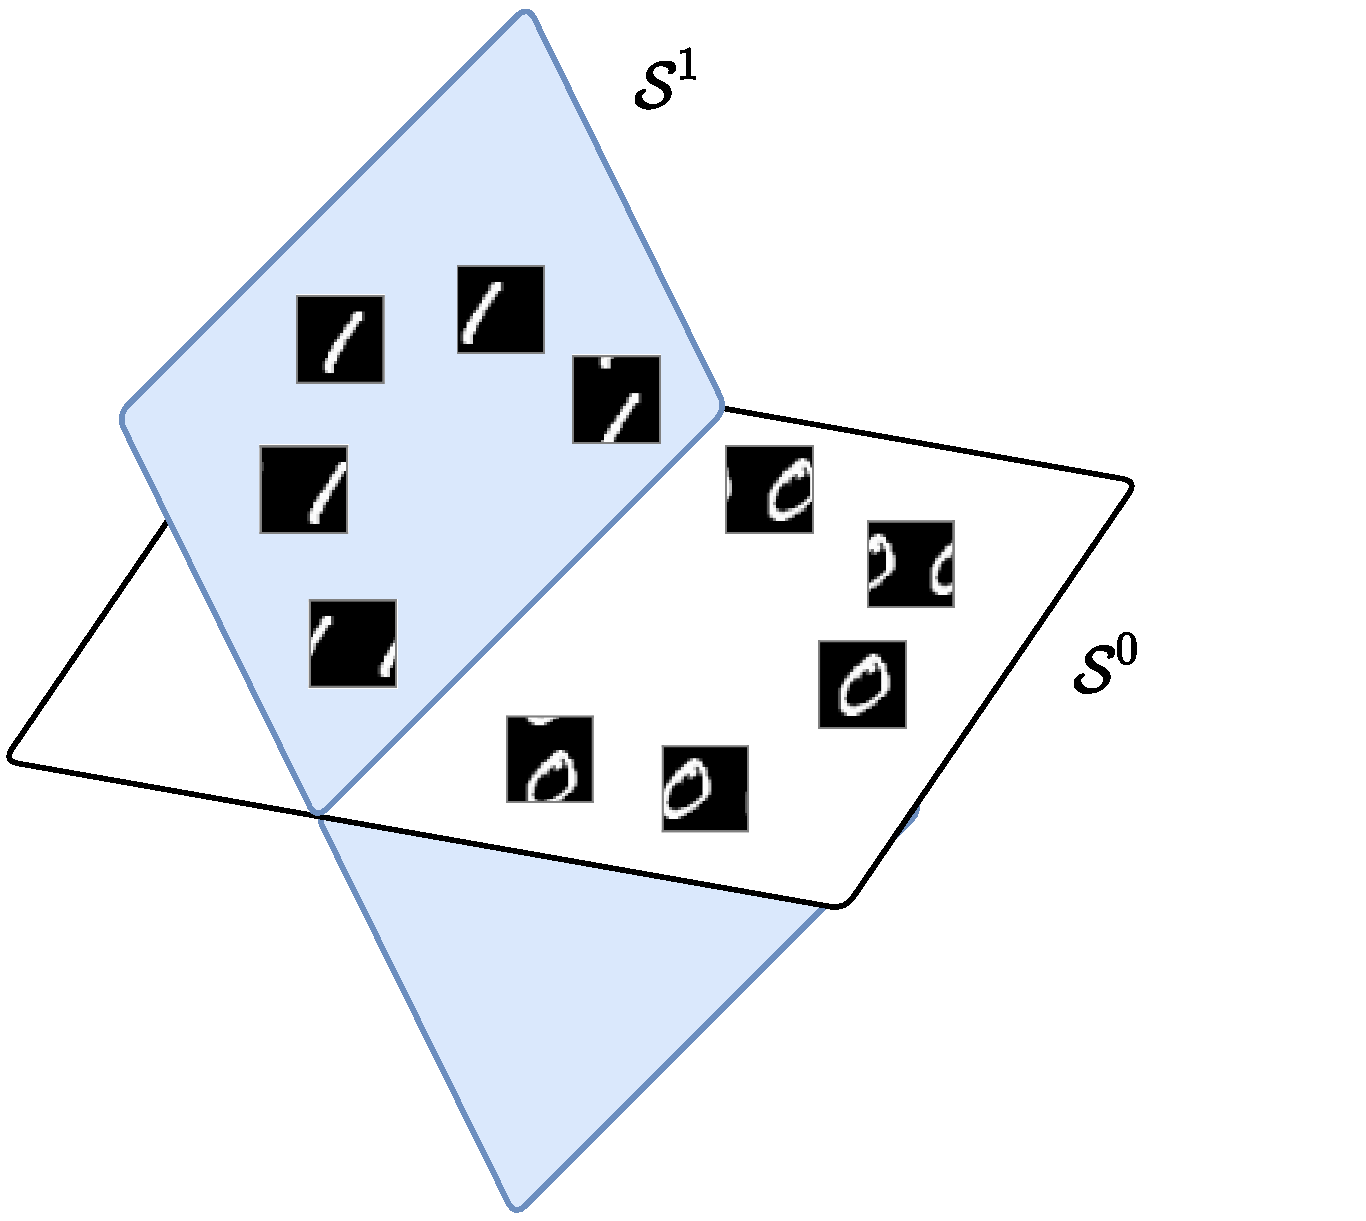
\includegraphics[width=\textwidth]{\toplevelprefix/chapters/chapter4/figs/ortho_diagram_2d.pdf}
    \end{subfigure}
    \caption{Ilustrarea reprezentării căutate care este echivariantă/invariantă la rotația imaginii (stânga) sau translație (dreapta): toate imaginile transformate ale fiecărei clase sunt mapate în același subspațiu care este incoerent cu alte subspații. Caracteristicile înglobate în fiecare subspațiu sunt echivariante la grupul de transformare, în timp ce fiecare subspațiu este invariant la astfel de transformări.}\label{fig:ortho-invariance-diagram} 
\end{figure}

\paragraph{Date Seriale 1D și Invarianță la Deplasare} Pentru a clasifica datele unidimensionale $\bm x = [x(0), x(1), \ldots, x(D-1)] \in \Re^D$ invariante sub deplasare, luăm $\mathbb{G}$ să fie grupul tuturor deplasărilor circulare. Fiecare observație $\bm x_i$ generează o familie $\{ \x_i \circ \mathfrak{g} \, | \, \mathfrak{g} \in \mathbb G \}$ de copii deplasate, care sunt coloanele matricei circulante $\circm(\bm x_i) \in \Re^{D \times D}$ dată de
\begin{equation}
\circm(\x) \,\doteq\, \left[ \begin{array}{ccccc} x(0) & x(D-1) & \dots & x(2) & x(1) \\ x(1) & x(0) & x(D-1) & \cdots & x(2) \\ \vdots & x(1) & x(0) &\ddots & \vdots \\ x(D-2) &  \vdots & \ddots & \ddots & x(D-1) \\ x(D-1) & x(D-2) & \dots & x(1) & x(0)   \end{array} \right]  \in \Re^{D \times D}.
\end{equation}
Trimitem cititorul la \cite{Kra2012OnCM} pentru proprietățile matricelor circulante. Pentru simplitate, fie $\bm Z^1 \doteq [ \z_{1}^1, \dots, \z_{N}^1 ] = \X \in \Re^{d \times N}$.\footnote{Din nou, pentru a simplifica discuția, presupunem deocamdată că caracteristicile inițiale $\Z^1$ sunt $\X$ înseși, prin urmare au aceeași dimensiune $d$, adică $D=d$. Dar aceasta nu trebuie să fie cazul, deoarece vom vedea în curând că trebuie să ridicăm $\X$ la o dimensiune mai mare.} Atunci ce se întâmplă dacă construim ReduNet din familiile lor circulante $\circm(\bm Z^1) = \left[ \circm(\z_{1}^1), \dots, \circm(\z_{N}^1) \right] \in \Re^{d \times (dN)}$? Adică, vrem să comprimăm și să mapăm toate acestea în același subspațiu prin ReduNet. 

Observați că acum matricea de covarianță a datelor: 
\begin{eqnarray}
\circm(\bm Z^1) \circm(\bm Z^1)^\top 
&=& \left[ \circm(\z_{1}^1), \dots, \circm(\z_{N}^1) \right] \left[ \circm(\z_{1}^1), \dots, \circm (\z_{N}^1) \right]^\top \nonumber \\
&=& \sum_{i =1}^N \circm(\z_{i}^1) \circm(\z_{i}^1)^\top \;\in \Re^{d\times d} 
\end{eqnarray}
asociată cu această familie de eșantioane este {\em automat} o matrice circulantă (simetrică). Mai mult, deoarece proprietatea circulantă este păstrată sub sume, inverse și produse, matricele $\bm E^1$ și $\bm C^1_k$ sunt, de asemenea, automat matrice circulante, a căror aplicare la un vector de caracteristici $\bm z \in \Re^d$ poate fi implementată folosind convoluția circulară „$\circledast$".
În mod specific, avem următoarea propoziție. 

\begin{proposition}[Structuri de convoluție ale $\bm E^1$ și $\bm C^1_k$]
Matricea 
\begin{equation}
    \bm E^1 = \alpha\big(\bm I + \alpha \circm(\bm Z^1) \circm(\bm Z^1)^\top \big)^{-1}
\end{equation}
este o matrice circulantă și reprezintă o convoluție circulară: 
$$\bm E^1 \z = \bm e_1 \circledast \z,$$ 
unde $\bm e_1 \in \Re^d$ este primul vector coloană al $\bm E^1$ și „$\circledast$" este convoluția circulară definită ca
\begin{equation*}
    (\bm e_1 \circledast \bm z)_{i} \doteq \sum_{j=0}^{d-1} e_1(j) x(i+ d-j \,\, \textsf{mod} \,\,d).
\end{equation*}
În mod similar, matricele $\bm C^1_k$ asociate cu orice subseturi ale $\bm Z^1$ sunt, de asemenea, convoluții circulare. 
\label{prop:circular-conv-1}
\end{proposition}

Această propoziție arată că, sub presupunerea invarianței la deplasare, operatorii derivați $\bm E^1$ și $\bm C^1_k$ devin în mod natural {\em convoluții circulare}. Din pacate, semnalele $\bm x_i \in \Re^D$ sunt de obicei de dimensiune prea mică pentru ca construcția de mai sus să funcționeze bine în practică---până și numerele cu cifre unice MNIST au dimensiune $D = 784$, ceea ce nu lasă prea mult loc de manevră pentru clustering: cel mult ar putea fi doar câțiva subspații liniare independente în $\Re^{784}$, departe de a fi suficient pentru a distinge cele zece cifre. Așa cum am sugerat în \Cref{subsec:lifting}, trebuie să {\em ridicăm} mai întâi semnalele (sau de fapt, măcar transformarea lor în domeniul frecvenței) la o reprezentare de dimensiune mai mare pentru ca obiectivul MCR$^2$ să funcționeze. Din punct de vedere conceptual, ridicarea poate fi văzută ca aplicarea unei măsuri netede de core (de exemplu, sinus și cosinus) la semnalul de intrare. 

O modalitate naturală de a realiza o astfel de ridicare este de a utiliza {\em măsuri ridicate circulante} ale semnalului. În analiză, măsuri ridicate sunt adesea asociate cu transformările semnalului cu nuclee, $\bm K \bm x$, unde $\bm K$ este o matrice Toeplitz bandată. De exemplu, pentru $D=3$ și $p=5$, cu $\bm x = [x(0), x(1), x(2)]^\top$, măsurarea ridicată circulantă ar fi:
\begin{equation}
    \mathcal{L}(\bm x) \doteq
    \begin{bmatrix}
        x(0) & x(2) & x(1) & 0 & 0\\
        x(1) & x(0) & x(2) & x(1) & 0\\
        x(2) & x(1) & x(0) & x(2) & x(1)\\
        0 & x(2) & x(1) & x(0) & x(2)\\
        0 & 0 & x(2) & x(1) & x(0)
    \end{bmatrix}
    \in \mathbb{R}^{p \times p}.
\end{equation}

\paragraph{Caracteristici Ridicate Multi-Canal și Invarianță la Deplasare.} 
Când semnalele sunt de dimensiune scăzută, ridicarea nu doar că facilitează învățarea structurilor multi-subspații, dar poate fi, de asemenea, realizată prin tehnici populare existente din învățarea profundă. Măsurarea ridicată circulantă generalizată, aplicată la un semnal de intrare $\bm x_i \in \Re^D$, poate fi reformulată și rescrisă ca mai multe aplicații de convoluții (ca \textit{filtre} sau \textit{canale}) cu dimensiuni diferite de nucleu, urmate de zero-padding.\footnote{Deși poate părea confuz matematic, ``zero-padding'' este deja o practică standard în straturile de convoluție ale rețelelor profunde moderne. Zero-padding-ul pur și simplu corespunde transformării observațiilor circulante într-o matrice Toeplitz. Cu toate acestea, aici zero-padding este aplicat \textit{după} convoluție pentru a menține diferitele canale la aceeași dimensiune, care diferă de aplicațiile obișnuite în rețelele profunde moderne \citep{he2016deep} unde se aplică \textit{înainte} de convoluție pentru a menține dimensiunea intrării.} Mai precis, măsurarea ridicată poate fi reprezentată ca aplicarea a $S$ filtre de convoluție $\{\bm{w}_s \in \Re^{d_s}\}_{s=1}^S$ la semnalul 1D $\bm x$, urmată de o operație de zero-padding. Aceasta rezultă într-o matrice ridicată $\bm M \in \Re^{S \times d}$, unde fiecare rând $\bm{m}_s^\top \in \Re^{d}$ reprezintă semnalul filtrat și umplut cu zero:
\begin{equation}
    \bm{m}_s^\top = \text{ZeroPad}\Big( \bm{w}_s * \bm{x} \Big) \in \Re^{d},
\end{equation}
și stivuind toate aceste măsuri ridicate: $\bm M = [\bm{m}_1, \ldots, \bm{m}_S ] \in \Re^{S \times d}$, care poate fi interpretată ca o hartă de caracteristici 1D cu $S$ canale. Avantajul nostru este că nu sunt necesare \textit{două} copii ale datelor în matrice (așa cum se arată în ecuația de mai sus).

Alegerea măsurilor ridicate nu este unică. Tehnici precum transformata Fourier rapidă (FFT), transformata cosinus discretă (DCT) sau transformata wavelet (DWT) servesc ca alternative bune. Ele pot fi văzute ca aplicarea de filtre de convoluție sinusoidale, cosinus sau wavelet ortogonale la semnalul de intrare. Atât timp cât măsurarea ridicată este invariantă la deplasare, structura convoluțională a $\bm E^1$ și $\bm C^1_k$ este păstrată. Aceasta este esența multor metode clasice de procesare a semnalelor digitale, precum și a multor rețele populare anterioare, cum ar fi ScatteringNet, care folosește wavelets \cite{scattering-net}.

\paragraph{Caracteristici Ridicate Rare pentru Reprezentare Separabilă.}
O modalitate alternativă de a vedea de ce ar trebui să ridicăm semnalele de dimensiune scăzută la o dimensiune mai mare este prin perspectiva sparsității în loc de separabilitatea subspațiului. De obicei, un semnal sau o imagine este generat dintr-un proces puternic neliniar care poate fi văzut ca transformare a unui cod rar de dimensiune mai mare în spațiul de observație de dimensiune mai scăzută. Dacă semnalele (sau imaginile) din aceeași clasă partajează anumite motive sau nuclee generatoare comune, atunci ele sunt susceptibile de a fi reprezentate ca convoluții ale acestor motive cu unele coduri rare. Mai precis, pentru semnale $\bm x = [x(1), x(2), \ldots, x(D)]^\top \in \Re^D$ din clasa $k$, presupunem că există un set de dicționare convoluționale $\bm D_k = [\bm d_{k,1}, \ldots, \bm d_{k,c}] \in \Re^{D\times c}$ unde $c$ este numărul de nuclee în dicționar, astfel încât
\begin{equation}
    \x = \bm d_{k,1} \circledast z_1 + \ldots + \bm d_{k,c} \circledast z_c = \circm(\bm{D}_k)\z,
\end{equation}
pentru un anumit vector rar $\z$. Semnalele din clase diferite sunt apoi generate de dicționare diferite ale căror atomi (sau motive) sunt incoerente unul față de celălalt. Datorită incoerenței, semnalele dintr-o clasă este puțin probabil să fie reprezentate rar de atomii din orice altă clasă. Prin urmare, toate semnalele pot fi reprezentate ca
\begin{equation}
\x = \big[\circm(\bm{D}_1), \circm(\bm{D}_2), \ldots, \circm(\bm{D}_K)\big] \bar \z,
\end{equation}
unde $\bar \z$ este rar.\footnote{Observați că modele similare de reprezentare rară au fost propuse și folosite de mult timp în scopuri de clasificare în aplicații precum recunoașterea facială, demonstrând o eficacitate excelentă \cite{Wright:2009,wagner2012toward}. Recent, modelul de codare rară convoluțională a fost propus de \cite{papyan2017convolutional} ca un cadru pentru interpretarea structurilor rețelelor convoluționale profunde.} Există o vastă literatură despre cum să învățăm cele mai compacte și optime dicționare de rarefiere din datele eșantion, de exemplu \cite{li2019multichannel,qu2019nonconvex} și ulterior să rezolvăm problema inversă și să calculăm codul rar asociat $\z$ sau $\bar \z$. Studii recente ale \cite{qu2020nonconvex,Qu2020Geometric} arată chiar că în condiții largi problema învățării dicționarului convoluțional poate fi rezolvată efectiv și eficient. 

Cu toate acestea, pentru sarcini precum clasificarea, nu suntem neapărat interesați de dicționarul optim precis, nici de codul rar precis pentru fiecare semnal individual. Suntem în principal interesați dacă în mod colectiv setul de coduri rare pentru fiecare clasă sunt adecvat separabile de cele ale altor clase. Sub presupunerea modelului generativ rar, dacă nucleele de convoluție $\{\bm k_c\}_{c=1}^C$ se potrivesc bine cu „transpusa" sau „inversa" dicționarelor de rarefiere de mai sus $\bm D = [\bm D_1, \ldots, \bm D_K]$, cunoscute și sub numele de {\em filtre de analiză} \cite{Cosparse-Nam,Analysis-Filter}, semnalele dintr-o clasă vor avea doar răspunsuri ridicate la un subset mic de astfel de filtre și răspunsuri scăzute la altele (datorită presupunerii de incoerență). Cu toate acestea, în practică, adesea un număr suficient de mare de, să zicem $C$, filtre aleatorii $\{\bm k_c\}_{c=1}^C$ este suficient pentru a asigura că caracteristicile extrase cu $C$-canale
\begin{equation}
\big[\bm k_1 \circledast \x, \bm k_2 \circledast \x, \ldots, \bm k_C \circledast \x\big]^\top = \big[\circm(\bm k_1) \x, \ldots, \circm(\bm k_C) \x \big]^\top \in \Re^{C\times d}
\end{equation}
pentru clase diferite au modele de răspuns diferite la filtre diferite, făcând astfel diferite clase separabile \cite{chan2015pcanet}. 

Prin urmare, în cadrul nostru, într-o mare măsură numărul de canale (sau lățimea rețelei) joacă cu adevărat rolul de {\em resursă statistică}, în timp ce numărul de straturi (adâncimea rețelei) joacă rolul de {\em resursă computațională}. Teoria detectării comprimate caracterizează precis câte măsurători sunt necesare pentru a păstra structurile intrinseci de dimensiune redusă (inclusiv separabilitatea) ale datelor \cite{Wright-Ma-2021}.

\begin{figure}[t]
	\centerline{
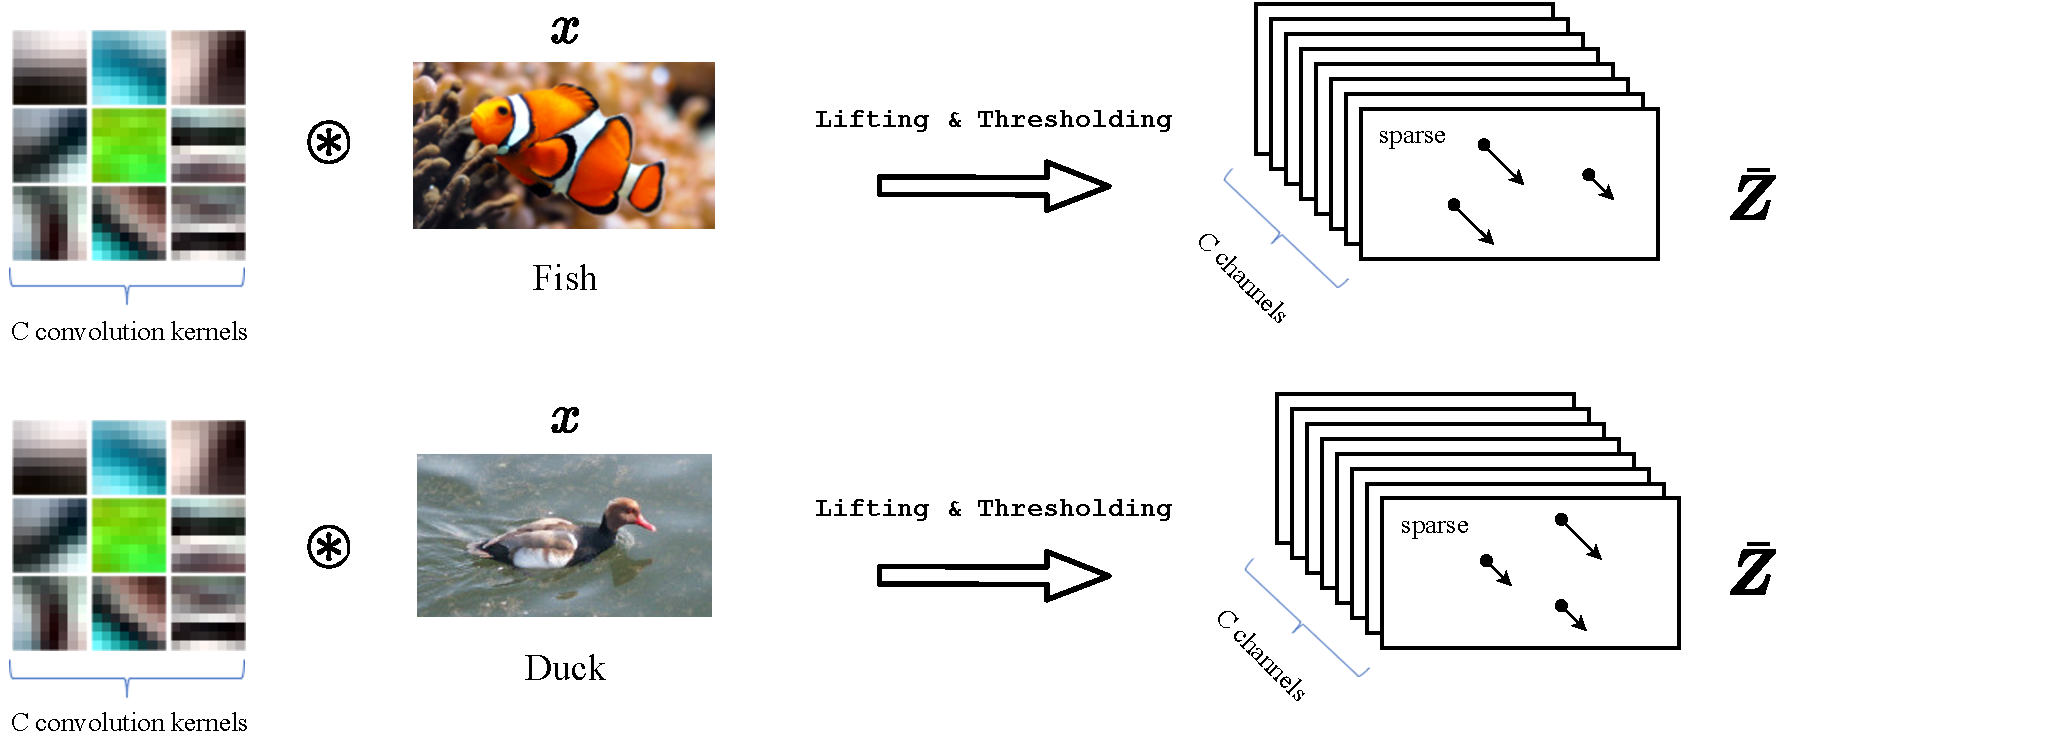
\includegraphics[width=0.95\textwidth]{\toplevelprefix/chapters/chapter4/figs/sparse-lifting.pdf}}
\caption{Estimarea codului rar $\bar{\bm z}$ al unui semnal de intrare $\bm x$ (o imagine aici) prin luarea convoluțiilor cu nuclee multiple $\bm k_c$ și apoi rarefiere.}
		\label{fig:multi-channel-sparse-lifting}
\end{figure}
Răspunsurile multi-canal $\bar \z$ ar trebui să fie rare. Deci, pentru a aproxima codul rar $\bar \z$, putem lua o {\em prag neliniar de promovare a sparsității} pe intrări, să zicem $\bm \tau(\cdot)$, pe ieșirile filtrului de mai sus prin setarea răspunsurilor scăzute (să zicem valoarea absolută sub $\epsilon$) sau negative la zero:
\begin{equation}
\bar \z \doteq \bm \tau \left( \big[\circm(\bm k_1) \x, \ldots, \circm(\bm k_C) \x \big]^\top \right) \in \Re^{C \times d}.
\label{eqn:sparse-lifting}
\end{equation} 
\Cref{fig:multi-channel-sparse-lifting} ilustrează ideile de bază. Se poate referi la \cite{Analysis-Filter} pentru un studiu mai sistematic asupra proiectării operatorului de prag de rarefiere. Cu toate acestea, aici nu suntem atât de interesați să obținem cele mai bune coduri rare atât timp cât codurile sunt suficient de separabile. Prin urmare, operatorul neliniar $\bm \tau$ poate fi ales simplu să fie un prag moale sau un ReLU. 
Aceste caracteristici presupus rare $\bar \z$ pot fi presupuse a se afla pe o subvarietate (neliniară) de dimensiune mai mică a $\mathbb{R}^{dC}$, care poate fi linearizată și separată de celelalte clase prin straturile ReduNet ulterioare, așa cum este ilustrat mai târziu în \Cref{fig:learn-to-classify-diagram}. 

ReduNet-ul construit din versiunea circulantă a acestor caracteristici multi-canal $\bar\Z \doteq [\bar \z_1, \ldots, \bar \z_N] \in \Re^{C \times d \times N}$, adică $\circm(\bar\Z) \doteq [ \circm(\bar\z_1), \dots, \circm(\bar\z_N)] \in \Re^{dC \times dN}$, păstrează proprietățile bune de invarianță descrise mai sus: operatorii liniari, acum notați ca $\bar{\bm E}$ și $\bar{\bm C}_k$, rămân bloc circulante și reprezintă {\em convoluții circulare 1D multi-canal.}
În mod specific, avem următorul rezultat.
\begin{proposition}[Structuri de convoluție multi-canal ale $\bar{\bm E}$ și $\bar{\bm C}_k$]
Matricea 
\begin{equation}
\label{eq:def-E-bar}
\bar{\bm E} \doteq \alpha\left(\bm I + \alpha\, \circm(\bar\Z) \circm(\bar\Z)^\top \right) ^{-1}  
\end{equation}
este bloc circulantă, adică,
\begin{equation*}
    \bar{\bm E} = 
    \left[\begin{matrix}
        \bar{\bm E}_{1, 1} & \cdots & \bar{\bm E}_{1, C}\\
        \vdots & \ddots & \vdots \\
        \bar{\bm E}_{C, 1} & \cdots & \bar{\bm E}_{C, C}\\
    \end{matrix}\right] \in \Re^{dC \times dC},
\end{equation*}
unde fiecare $\bar{\bm E}_{c, c'}\in \Re^{d \times d}$ este o matrice circulantă. Mai mult, $\bar{\bm E}$ reprezintă o convoluție circulară multi-canal, adică, pentru orice semnal multi-canal $\bar\z \in \Re^{C \times n}$ avem 
$$\bar{\bm E} \cdot \textsf{vec}(\bar\z) = \textsf{vec}( \bar{\bm e} \circledast \bar\z).$$ 
În cele de mai sus, $\bar{\bm e} \in \Re^{C \times C \times d}$ este un nucleu convoluțional multi-canal cu $\bar{\bm e}[c, c'] \in \Re^{d}$ fiind primul vector coloană al $\bar{\bm E}_{c, c'}$, și $\bar{\bm e} \circledast \bar\z \in \Re^{C \times d}$ este convoluția circulară multi-canal definită ca
\begin{equation*}
    (\bar{\bm e} \circledast \bar\z)[c] \doteq \sum_{c'=1}^C \bar{\bm e}[c, c'] \circledast \bar{\z}[c'], \quad \forall c = 1, \ldots, C.
\end{equation*}
În mod similar, matricele $\bar{\bm C}_k$ asociate cu orice subseturi ale $\bar{\bm Z}$ sunt, de asemenea, convoluții circulare multi-canal. 
\label{prop:multichannel-circular-conv-1}
\end{proposition}
Din \Cref{prop:multichannel-circular-conv-1}, ReduNet invariant la deplasare este o rețea convoluțională profundă pentru semnale 1D multi-canal prin construcție. Observați că chiar dacă nucleele de ridicare inițiale sunt separate \eqref{eqn:sparse-lifting}, inversa matricei în \eqref{eq:def-E-bar} pentru calcularea $\bar{\bm E}$ (similar pentru $\bar{\bm C_k}$) introduce „comunicare încrucișată" între toate cele $C$ canale.
Prin urmare, aceste convoluții multi-canal în general {\em nu} sunt separabile în adâncime, spre deosebire de rețelele Xception~\cite{Xception} care au fost odată sugerate pentru a simplifica rețelele neuronale convoluționale multi-canal.\footnote{Rămâne deschis ce structuri suplimentare asupra datelor ar duce la convoluții separabile în adâncime.} 

\begin{remark}[Reducerea Complexității Computaționale în Domeniul Frecvenței] 
Calculul $\bar{\bm E}$ în \eqref{eq:def-E-bar} necesită inversarea unei matrice de dimensiune $dC \times dC$, care în general are complexitatea $O(d^3C^3)$. Cu toate acestea, folosind faptul că o matrice circulantă poate fi diagonalizată de matricea Transformatei Fourier Discrete (DFT), complexitatea poate fi redusă semnificativ. După cum este arătat în \cite{chan2021redunet}, pentru a calcula $\bar{\bm E}$ și $\bar{\bm C}_k \in \Re^{dC \times dC}$, trebuie doar să calculăm în domeniul frecvenței inversa blocurilor $C\times C$ de $d$ ori, prin urmare complexitatea generală devine $O(dC^3)$.
    
\end{remark}




\paragraph{Arhitectura Generală a Rețelei și Comparație.} 
Urmând derivarea de mai sus, vedem că pentru a găsi o reprezentare discriminativă liniară (LDR) pentru mai multe clase de semnale/imagini care este invariantă la translație, codarea rară, o arhitectură multi-strat cu convoluții multi-canal, diferite activări neliniare și calculul spectrului devin toate componente {\em necesare} pentru atingerea obiectivului în mod efectiv și eficient. \Cref{fig:learn-to-classify-diagram} ilustrează procesul general de învățare a unei astfel de reprezentări prin reducerea ratei invariante pe codurile rare de intrare. 

\begin{figure}[t]
    \centering
    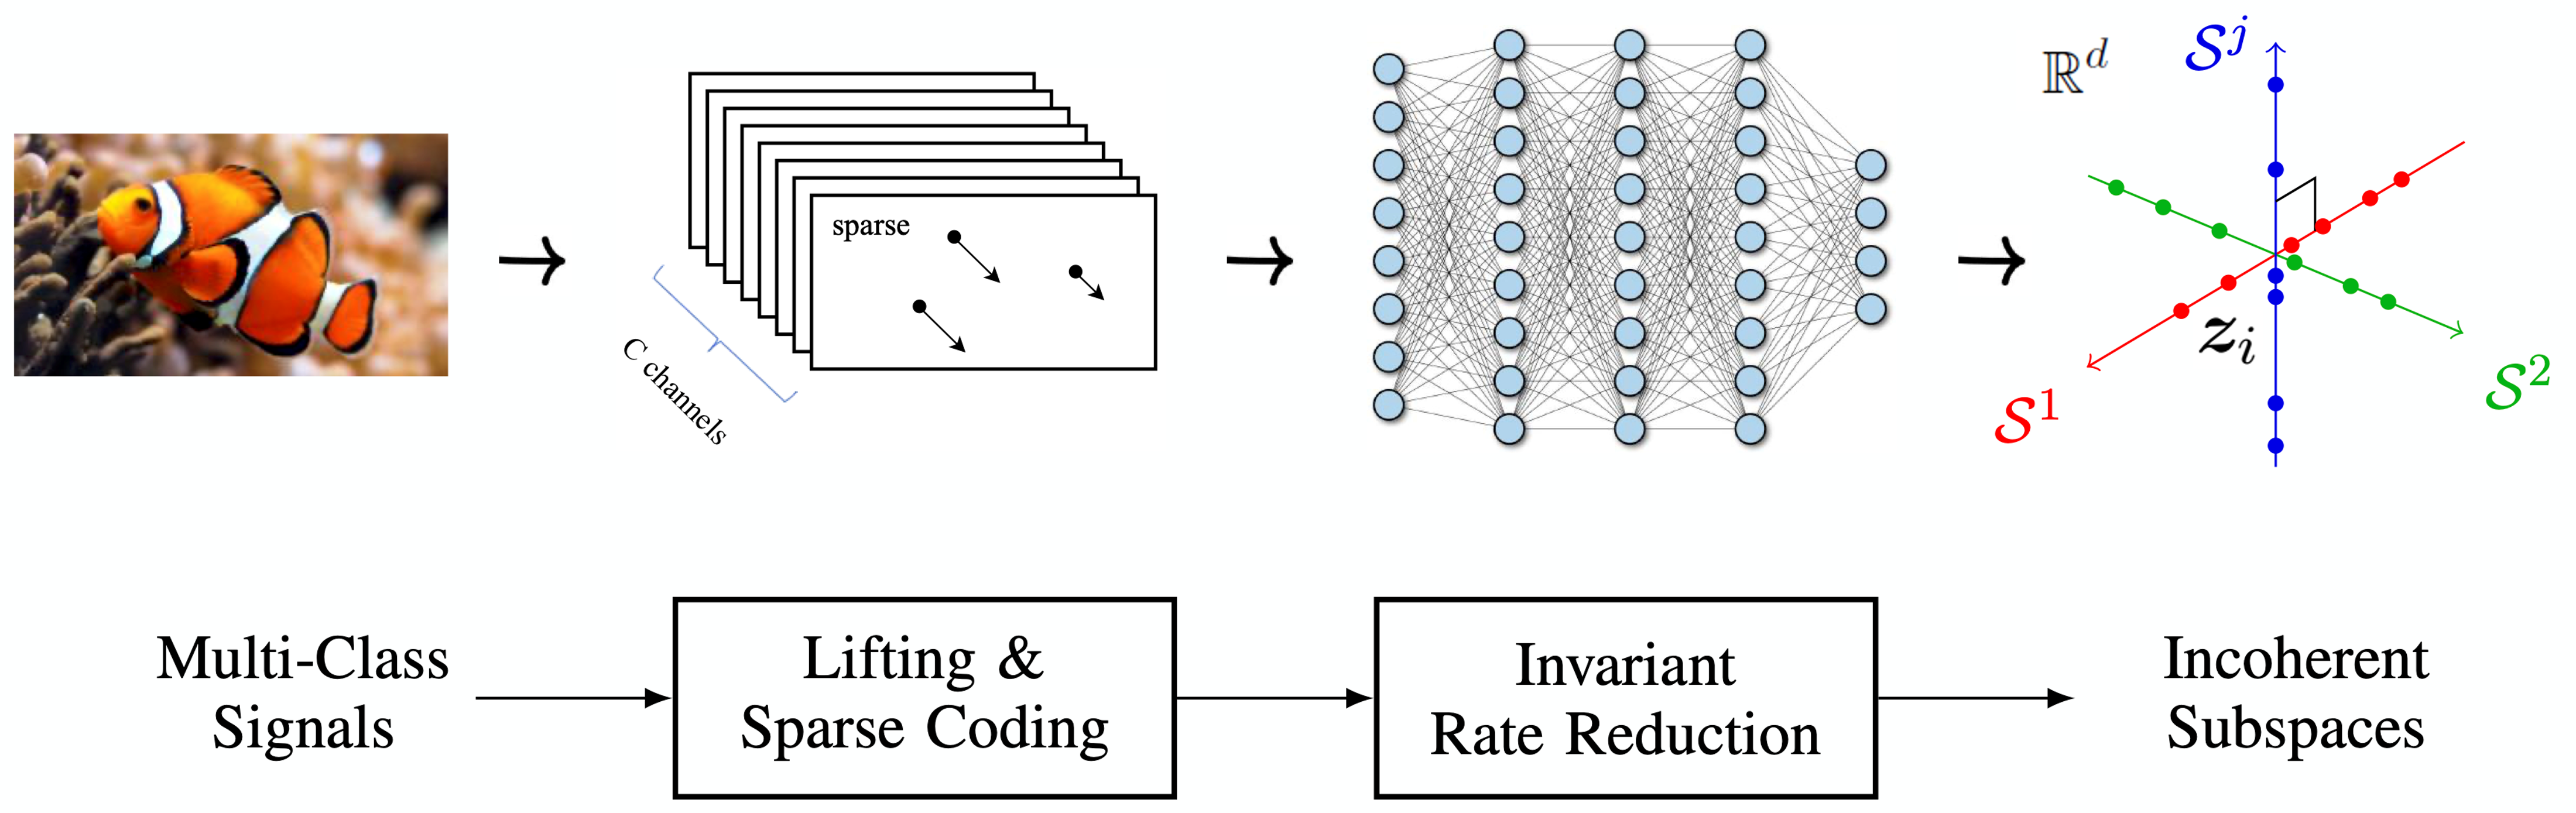
\includegraphics[width=0.98\linewidth]{\toplevelprefix/chapters/chapter4/figs/learn_to_classify_diagram_updated.png}
    \caption{Procesul general pentru clasificarea semnalelor multi-clasă cu invarianță la deplasare: Ridicare multi-canal, codare rară, urmată de un ReduNet de convoluție multi-canal pentru reducerea ratei invariante. Aceste componente sunt {\em necesare} pentru a mapa semnale multi-clasă invariante la deplasare la subspații (liniare) incoerente ca LDR. Notați că arhitecturile majorității rețelelor neuronale profunde moderne seamănă cu acest proces. LDR-ul astfel învățat facilitează sarcinile ulterioare precum clasificarea.}
    \label{fig:learn-to-classify-diagram}
\end{figure}


\begin{example}[Clasificarea Invariantă a Cifrelor]
Prezentăm în continuare performanța empirică a ReduNet-ului pe învățarea caracteristicilor invariante la \textit{rotație} pe setul de date real MNIST cu 10 clase. 
Impunem o grilă polară pe imaginea $\bm{x}\in\mathbb{R}^{H\times W}$, cu centrul său geometric fiind centrul grilei polare 2D (așa cum este ilustrat în \Cref{fig:samples-invariant-1d-mnist-diagram}). 
Pentru fiecare rază $r_i$, $i \in [C]$, putem eșantiona $\Gamma$ pixeli cu privire la fiecare unghi $\gamma_l =l\cdot({2\pi}/\Gamma)$ cu $l \in [\Gamma]$. 
Apoi, dat o imagine eșantion $\bm{x}$ din setul de date, reprezentăm imaginea în coordonata polară (eșantionată) ca un semnal multi-canal $\bm{x}_p \in\R^{\Gamma\times C}$.  
Scopul aici este să învățăm o reprezentare invariantă la rotație, adică ne așteptăm să învățăm $f(\cdot, \bm{\theta})$ astfel încât $\{f(\bm{x}_p \circ \mathfrak{g}, \bm{\theta})\}_{\mathfrak{g} \in\mathbb{G}}$ să se afle în același subspațiu, unde $\mathfrak{g}$ este deplasarea ciclică în unghiul polar.  
Folosim $N=100$ eșantioane de antrenament ($10$ din fiecare clasă) și setăm $\Gamma=200$, $C=15$ pentru eșantionarea polară. 
Efectuând eșantionarea de mai sus în coordonate polare, putem obține matricea de date $\bm{X}_p \in \mathbb{R}^{(\Gamma\cdot C) \times N}$. 
Pentru ReduNet, setăm numărul de straturi/iterații $L=40$, precizia $\epsilon=0.1$, dimensiunea pasului $\eta=0.5$. Înainte de primul strat, efectuăm ridicarea intrării prin convoluție circulantă 1D cu 20 de nuclee Gaussiene aleatorii de dimensiune 5.   

\begin{figure}[t]
    \begin{subfigure}[t]{0.3\textwidth}
        \centering
        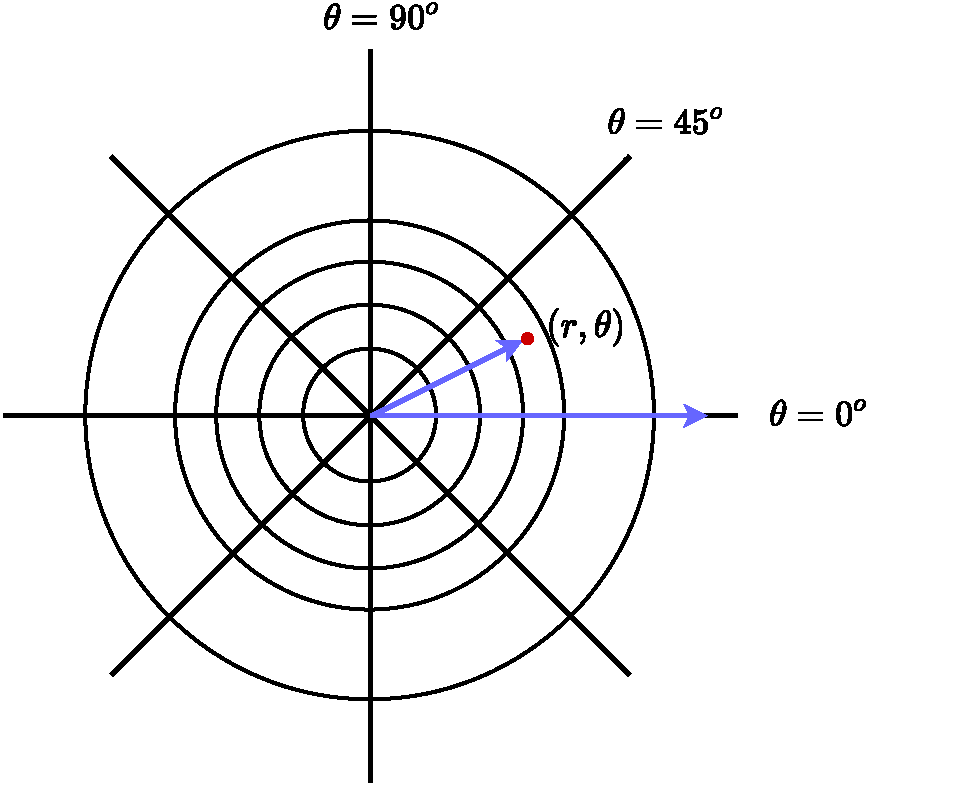
\includegraphics[width=\textwidth]{\toplevelprefix/chapters/chapter4/figs/1d-rotation.pdf}
        \caption{$\bm{X}_{\text{rotație}}$}
    \end{subfigure}
    \hfill
    \begin{subfigure}[t]{0.3\textwidth}
        \centering
        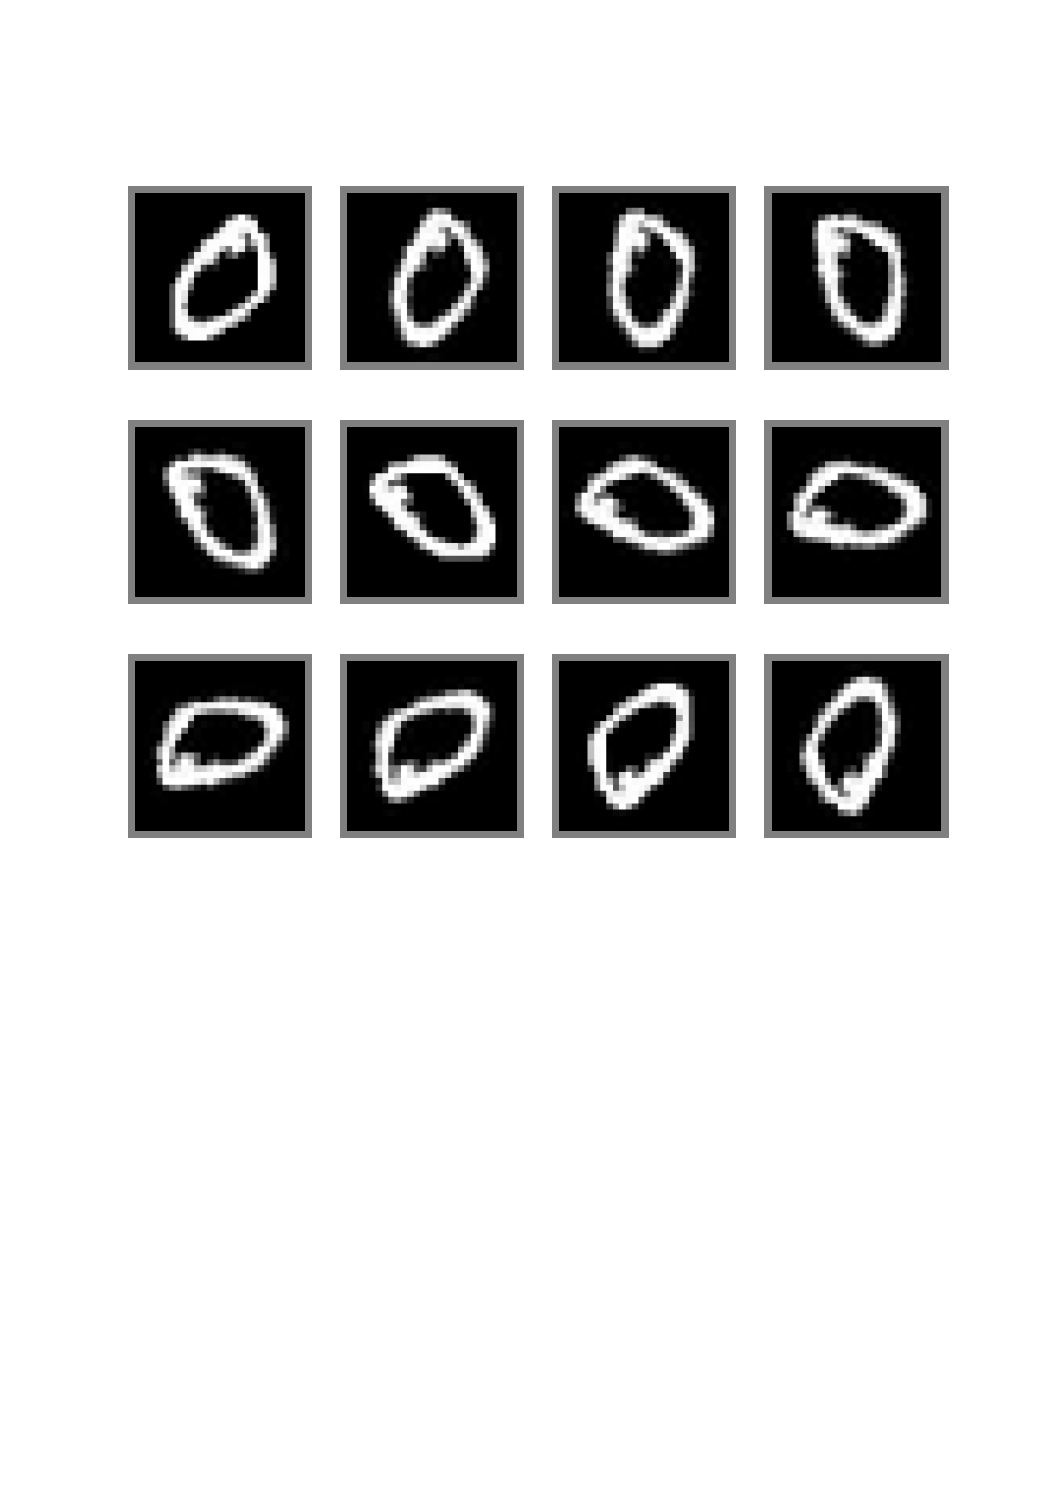
\includegraphics[width=\textwidth]{\toplevelprefix/chapters/chapter4/figs/mnist1d_img0.pdf}
        \caption{$\bm{Z}_{\text{rotație}}$}
    \end{subfigure}
    \hfill
    \begin{subfigure}[t]{0.3\textwidth}
        \centering
        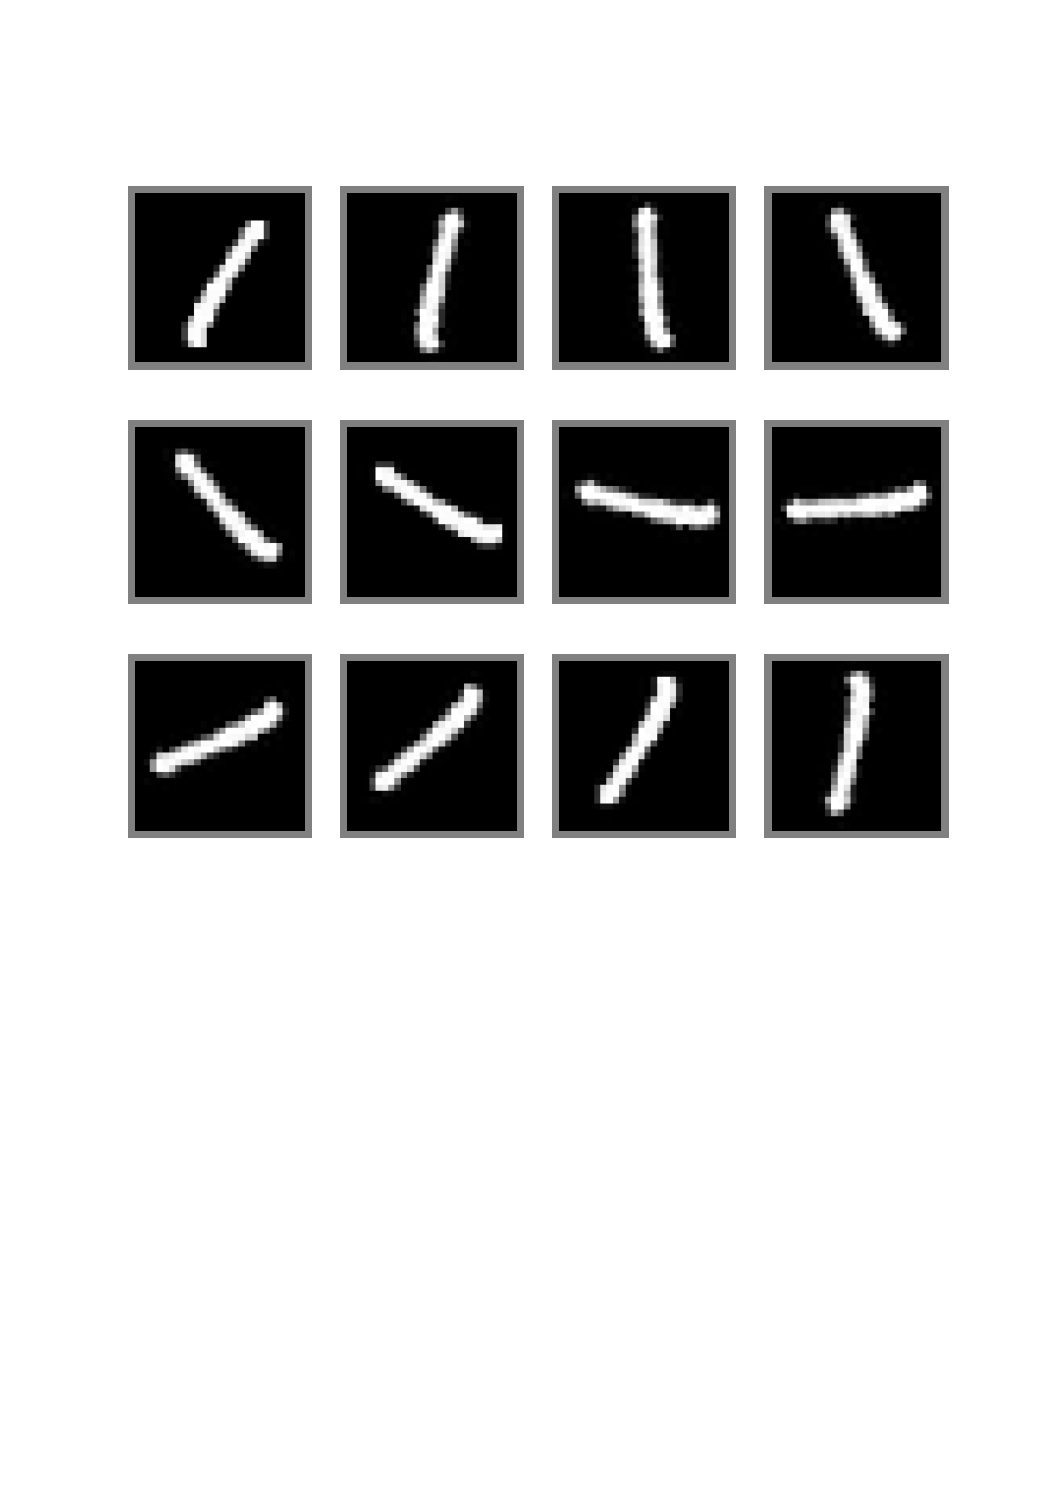
\includegraphics[width=\textwidth]{\toplevelprefix/chapters/chapter4/figs/mnist1d_img1.pdf}
        \caption{Pierdere}
    \end{subfigure}
    \caption{\small Exemple de imagini rotite ale cifrelor MNIST, fiecare cu 18$^{\circ}$. (\textbf{Stânga}) Diagramă pentru reprezentarea în coordonate polare; (\textbf{Dreapta}) Imagini rotite ale cifrei '0' și '1'.}
    \label{fig:samples-invariant-1d-mnist-diagram}
\end{figure}


Pentru a evalua reprezentarea învățată, fiecare eșantion de antrenament este augmentat cu 20 de versiuni rotite ale sale, fiecare deplasată cu pas=10. Calculăm similaritățile cosinus între intrările de antrenament augmentate $m \times 20$ $\bm{X}_{\text{rotație}}$ și rezultatele sunt prezentate în \Cref{fig:redu-invariant-1d-mnist-diagram} (\textbf{a}). 
Comparăm similaritățile cosinus între caracteristicile învățate ale tuturor versiunilor augmentate, adică $\bar{\bm{Z}}_{\text{rotație}}$ și rezumăm rezultatele în \Cref{fig:redu-invariant-1d-mnist-diagram} (\textbf{b}). 
După cum vedem, ReduNet-ul invariant la rotație astfel construit este capabil să mapeze datele de antrenament (precum și toate versiunile sale rotite) din cele 10 clase diferite în 10 subspații aproape ortogonale. Adică, subspațiile învățate sunt cu adevărat invariante la transformarea de deplasare în unghiul polar. În continuare, extragem aleatoriu alte $100$ de eșantioane de test urmate de aceeași procedură de augmentare. 
În \Cref{fig:redu-invariant-1d-mnist-diagram} (\textbf{c}), vizualizăm pierderea MCR$^{2}$ pe reprezentarea stratului $\ell$-lea a ReduNet-ului pe setul de date de antrenament și test. Din aceste rezultate, putem constata că ReduNet-ul construit este într-adevăr capabil să maximizeze pierderea MCR$^{2}$ și să generalizeze la datele de test.



\begin{figure}[t]
    \begin{subfigure}[t]{0.3\textwidth}
        \centering
        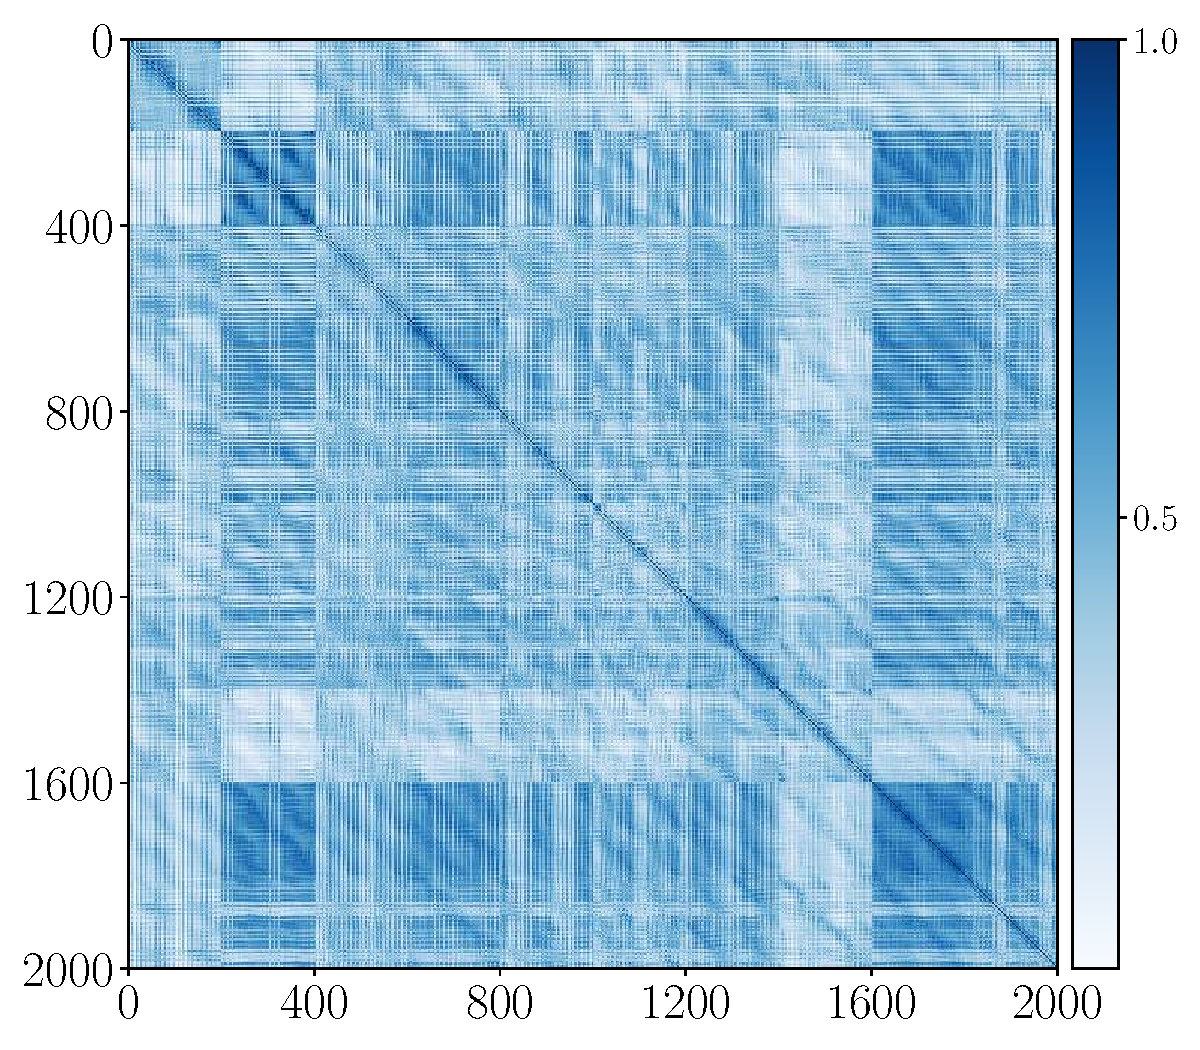
\includegraphics[width=\textwidth]{\toplevelprefix/chapters/chapter4/figs/mnist1d-heatmap-X_translate_train_all.pdf}
        \caption{$\bm{X}_{\text{rotație}}$}
    \end{subfigure}
    \hfill
    \begin{subfigure}[t]{0.3\textwidth}
        \centering
        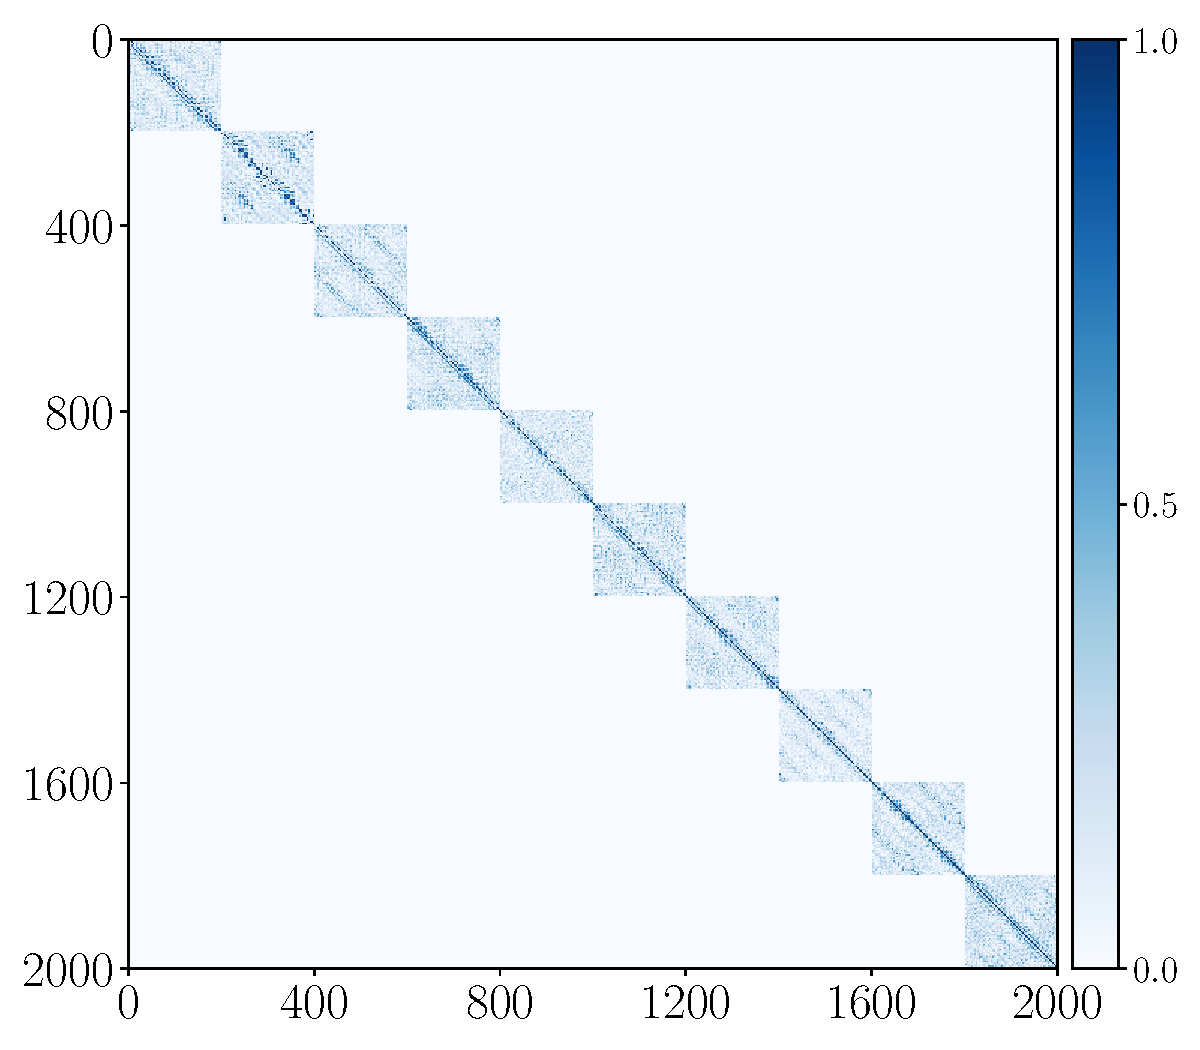
\includegraphics[width=\textwidth]{\toplevelprefix/chapters/chapter4/figs/mnist1d-heatmap-Z_translate_train_all.pdf}
        \caption{$\bm{Z}_{\text{rotație}}$}
    \end{subfigure}
    \hfill
    \begin{subfigure}[t]{0.32\textwidth}
        \centering
        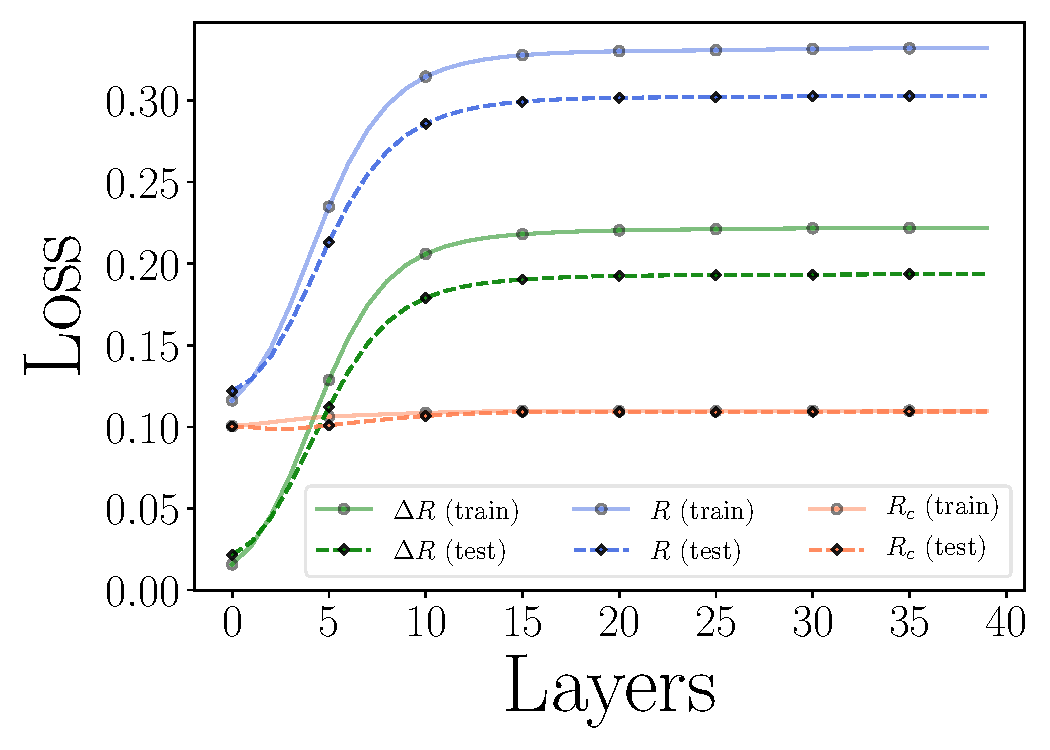
\includegraphics[width=\textwidth]{\toplevelprefix/chapters/chapter4/figs/mnist1d-loss-traintest.pdf}
        \caption{Pierdere}
    \end{subfigure}
    \caption{\small (a)(b) sunt hărți de căldură ale similarității cosinus între datele de antrenament rotite $\bm{X}_{\text{rotație}}$ și caracteristicile învățate $\bar{\bm{Z}}_{\text{rotație}}$ pentru invarianța la rotație. (d) vizualizează pierderile MCR$^2$ de antrenament/validare pe straturi.}
    \label{fig:redu-invariant-1d-mnist-diagram}
\end{figure}

\end{example}








\section{Rețele Profunde pentru Reprezentări Parcimonioase prin Optimizare Desfășurată}\label{sec:deep-sparse-coding}

În secțiunea anterioară, am văzut cum putem construi o rețea profundă prin desfășurarea optimizării pentru obiectivul de reducere a ratei de codare pentru subspații de dimensiune redusă. 
Aceasta poate gestiona eficient structuri (liniare) de dimensiune redusă. 
Cu toate acestea, în multe scenarii, semnalele cu care avem de-a face pot fi mai bine caracterizate prin reprezentări rare într-un dicționar supracomplet, așa cum a fost discutat în \Cref{ch:classic}. În această secțiune, ne concentrăm pe învățarea reprezentărilor pentru date care sunt generate rar de un dicționar și extindem cadrul nostru de compresie pentru a acomoda astfel de structuri rare.

\subsection{Sparse Lifting și Ridicare Spațială}
\label{subsec:lifting}

Ideea de bază este că ne putem ridica sau mapa datele în spațiul în care ele sunt reprezentate rar și apoi să aplicăm obiectivul de reducere a ratei pe reprezentările rare pentru a le separa în subspații mai coerente între diferite clase. Aceasta este de fapt o practică extrem de comună în învățarea profundă și procesarea imaginilor, cunoscută adesea sub diferite denumiri precum {\em extragerea caracteristicilor}, sau {\em înglobarea spațială} a tokenurilor. În mod specific, presupunem că există o transformare a domeniului $\varphi(\cdot)$ care mapează datele $\x$ în reprezentări de dimensiune mai mare (rare):
\begin{equation}
    \varphi: \x \in \Re^D \mapsto \z \in \Re^p, \quad p \gg D.
\end{equation}

Designul transformării de ridicare este strâns legat de asumpția modelului generativ sau proprietățile datelor. De exemplu, pentru imagini naturale, transformările comune includ patch-uri de imagine (ferestre glisante), wavelets sau alte baze multi-rezoluție. Pentru date secvențiale, aceasta ar putea fi transformări Fourier sau codificări poziționale. 

În cadrul învățării profunde moderne, ridicarea este adesea realizată prin straturi convoluționale învățate sau straturi de embedding. Totuși, pentru analiza noastră principială, considerăm mapări de ridicare mai interpretabile care conservă structura de grup a datelor, menținând în același timp sparsitatea reprezentării.

\begin{figure}[t]
    \centering
    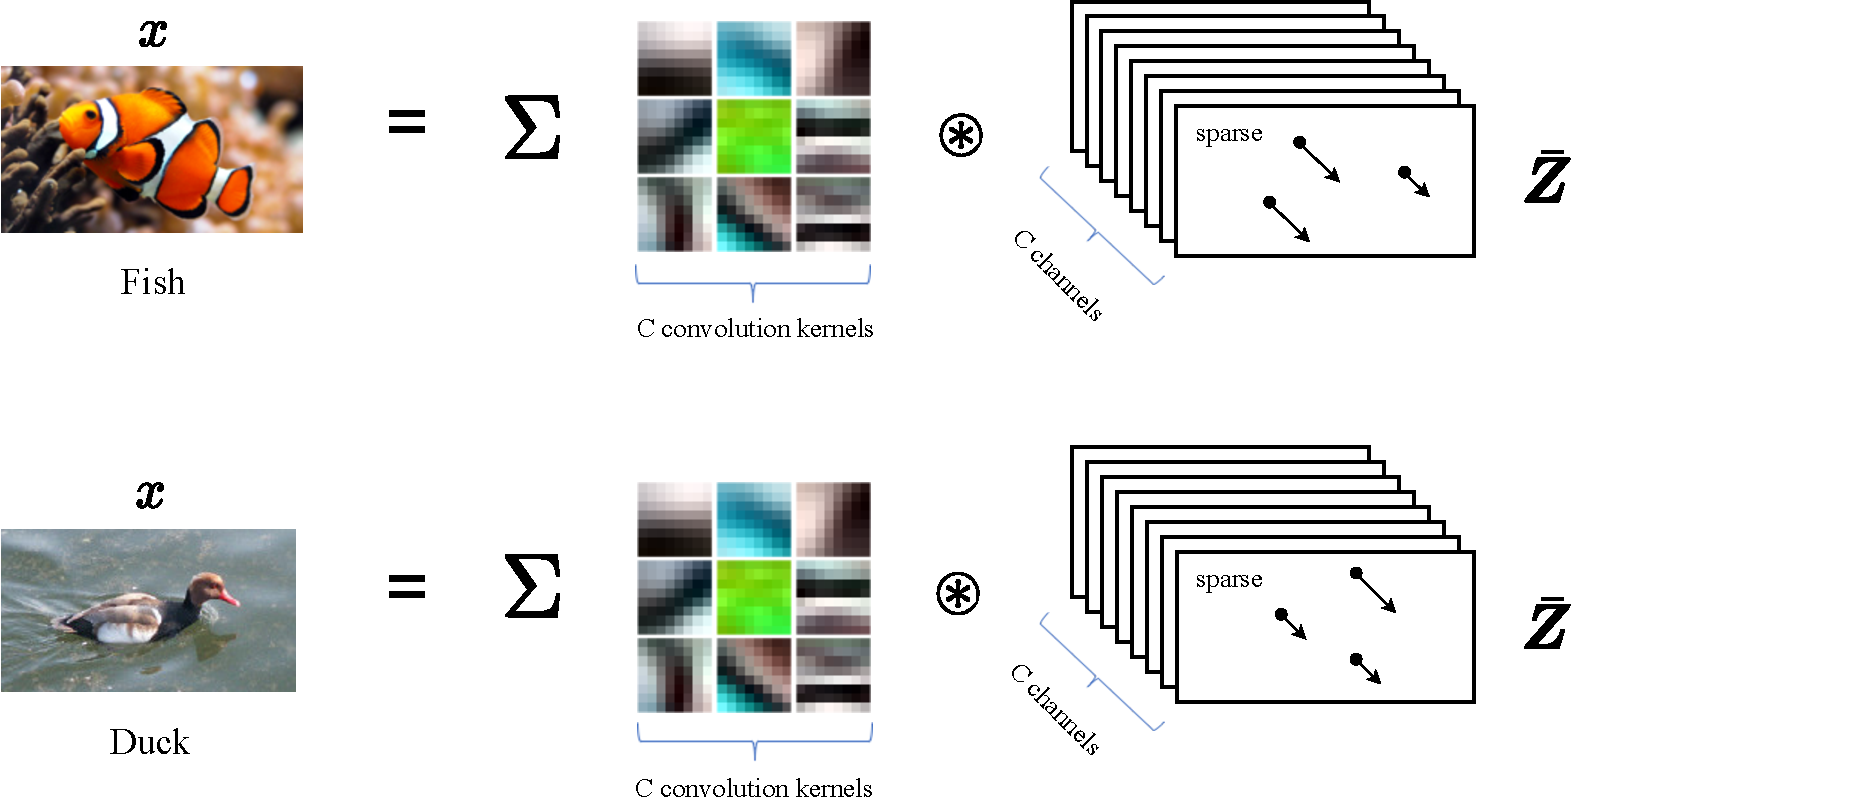
\includegraphics[width=0.9\linewidth]{\toplevelprefix/chapters/chapter4/figs/sparse-representation.pdf}
    \caption{Ilustrarea ridicării rare: datele originale $\x$ sunt transformate într-o reprezentare rară de dimensiune înaltă $\z$ prin transformarea de ridicare $\varphi(\cdot)$. Reprezentarea rară facilitează separarea între diferite clase prin maximizarea reducerii ratei de codare.}
    \label{fig:sparse-lifting-illustration}
\end{figure}

\subsection{Optimizare Desfășurată pentru Codare Rară}

Presupunem că datele noastre $\x$ pot fi reprezentate ca o combinație rară de atomi dintr-un dicționar $\bm D \in \Re^{D \times p}$:
\begin{equation}
    \x = \bm D \z + \bm \varepsilon,
\end{equation}
unde $\z \in \Re^p$ este un vector rar (majoritatea intrărilor sunt zero) și $\bm \varepsilon$ este zgomot. Problema de a găsi cea mai rară reprezentare poate fi formulată ca:
\begin{equation}\label{eq:sparse-coding}
    \min_{\z} \frac{1}{2}\|\x - \bm D \z\|_2^2 + \lambda \|\z\|_1,
\end{equation}
unde $\|\z\|_1 = \sum_{i=1}^p |z_i|$ este norma $\ell_1$ care promovează sparsitatea.

Pentru a rezolva această problemă de optimizare, putem folosi algoritmul de prag iterativ de contracție (ISTA), care alternează între pași de gradient și operații de prag moale:
\begin{equation}\label{eq:ista}
    \z^{\ell+1} = \mathcal{S}_{\lambda\eta}\left(\z^\ell - \eta \bm D^\top(\bm D \z^\ell - \x)\right),
\end{equation}
unde $\mathcal{S}_{\tau}(\cdot)$ este operatorul de prag moale definit ca:
\begin{equation}
    \mathcal{S}_{\tau}(z) = \text{sign}(z) \cdot \max(|z| - \tau, 0).
\end{equation}

Desfășurând iterațiile ISTA, obținem o rețea profundă în care fiecare strat efectuează o operație de codare rară. Aceasta seamănă cu arhitectura Learned ISTA (LISTA), unde parametrii algoritmului sunt învățați din date prin retropropagare în loc să fie fixați. Reprezentarea finală rară poate fi apoi utilizată pentru sarcinile ulterioare.








\section{Transformatoare cu Cutie Albă din Optimizare Desfășurată}\label{sec:chap4-white-box-transformer}
După cum am văzut în secțiunea anterioară, folosim problema clasificării pentru a oferi o interpretare riguroasă pentru caracteristicile arhitecturale principale ale rețelelor profunde populare precum ResNet și CNN: fiecare strat al acestor rețele poate fi văzut ca imitând un pas de gradient care crește obiectivul de reducere a ratei (sau câștigul de informație). Această perspectivă duce, de asemenea, la un fapt oarecum surprinzător: parametrii și operatorii straturilor unei astfel de rețele profunde, ReduNet, pot fi calculați într-o manieră pur înainte.

În ciuda importanței teoretice și conceptuale a ReduNet, mai mulți factori o limitează să fie foarte practică. În primul rând, așa cum am discutat mai sus, costul computațional al calculării operatorilor matriciali în fiecare strat într-o manieră înainte poate fi foarte mare. În al doilea rând, operatorii astfel calculați pot să nu fie atât de eficienți în optimizarea obiectivului și ar putea dura mii de iterații (deci straturi). După cum am văzut în \Cref{sec:LISTA} pentru LISTA, aceste două probleme pot fi abordate permițând optimizarea acelor operatori și făcându-i învățabili prin retropropagare.\footnote{Sau, poate, printr-un amestec de optimizare înainte și înapoi.}

Setarea de clasificare supervizată în care a fost derivat ReduNet este, de asemenea, oarecum limitativă. În practică, o imagine ar putea să nu aparțină unei singure clase, deoarece poate conține mai multe obiecte. Prin urmare, ar fi mai general să presupunem că diferite regiuni ale imaginii aparțin unor modele diferite de dimensiune redusă (să zicem un Gaussian sau un subspațiu). După cum vom vedea, o astfel de generalizare ar duce la o arhitectură atât simplă, cât și generală, care unifică operațiile de reducere a ratei și de denoising pe care le-am văzut în capitolul anterior. Mai mult, arhitectura astfel obținută seamănă cu arhitectura populară Transformer.



\subsection{Optimizare Desfășurată pentru Reducerea Ratei Rare}



Considerăm o configurare generală de învățare asociată cu semnale din lumea reală. Fie \(\X = \mat{\x_{1}, \dots, \x_{N}} \in \bR^{D \times N}\) variabile aleatoare care reprezintă sursa noastră de date. În sarcinile de viziune, fiecare \(\x_{i} \in \bR^{D}\) este interpretat ca un \textit{token}, de obicei corespunzând unei petice de imagine. În sarcinile de limbaj, fiecare \(\x_{i} \in \bR^{D}\) este interpretat ca o \textit{înglobare de token}, adică o reprezentare vectorială continuă a unui token discret, cum ar fi un cuvânt sau subcuvânt.\footnote{Cu un ușor abuz de terminologie, ne referim atât la tokeni discreți, cât și la înglobările lor asociate, pur și simplu ca tokeni pe parcursul acestui capitol pentru comoditate.}
\(\x_{i}\)-urile pot avea structuri de corelație arbitrare. Folosim \(\Z = \mat{\z_{1}, \dots, \z_{N}} \in \bR^{d \times N}\) pentru a denota variabilele aleatoare care definesc reprezentările noastre, unde \(\z_{i} \in \bR^{d}\) este reprezentarea tokenului corespunzător \(\x_i \in \bR^{D}\).

\begin{remark}
    În transformatoare, fiecare eșantion de intrare este de obicei convertit într-o secvență de {\em tokeni}. Un token este o unitate de bază de informație derivată din intrarea brută: în procesarea limbajului natural, tokenii sunt de obicei cuvinte sau subcuvinte; în viziunea computerizată, ei corespund petelor de imagine; și în alte modalități, pot reprezenta pași de timp, locații spațiale sau alte unități specifice domeniului. O {\em înglobare de token} este o reprezentare vectorială continuă a unui token care servește ca intrare pentru un transformer. Ea mapează fiecare token la un punct într-un spațiu de dimensiune înaltă, permițând modelului să proceseze intrări simbolice folosind calcul numeric.
    O {\em reprezentare de token} este un vector care codifică informația semantică sau structurală a unui token, de obicei produs de straturile intermediare sau finale ale unui transformer. Aceste reprezentări sunt concepute pentru a captura caracteristici semnificative ale intrării care sunt utile pentru sarcini ulterioare, cum ar fi clasificarea, generarea sau regresia. Vă rugăm să consultați \Cref{sec:contrastive_learning} pentru mai multe detalii despre aceste concepte în implementări. 
\end{remark}


 
\paragraph{Obiectiv pentru Învățarea unei Reprezentări Structurate și Compacte.}
Urmând cadrul reducerii ratei \Cref{sec:chap4-white-box-model-via-unrolling}, susținem că scopul învățării reprezentărilor este de a găsi o mapare de caracteristici \(f
\colon \X \in \bR^{D \times N} \to \Z\in \bR^{d \times N}\) care transformă tokenii de intrare \(\{\bm x_i\}_{i=1}^N \subset \R^D\) cu o distribuție potențial neliniară și multi-modală în reprezentări de tokeni \textit{linearizate și compacte} (pe bucăți) \(\{\bm z_i\}_{i=1}^N \subset \bR^{d}\). În timp ce distribuția comună a reprezentărilor tokenilor \(\{\z_{i}\}_{i = 1}^{N}\) poate fi sofisticată (și specifică sarcinii), susținem în continuare că este rezonabil și practic să cerem ca distribuția marginală țintă a reprezentărilor individuale de tokeni să fie foarte comprimată și structurată, potrivită pentru codare compactă. În special, cerem ca distribuția să fie \textit{un amestec de distribuții Gaussiene de dimensiune redusă (să zicem \(K\))}, astfel încât Gaussiana \(k\)-a să aibă media \(\Zero \in \bR^{d}\), covarianța \(\vSigma_{k} \succeq \Zero \in \bR^{d \times d}\) și suport întins de baza ortonormată \(\vU_{k} \in \bR^{d \times p}\). 
Notăm $\vU_{[K]} = \{\vU_k\}_{k=1}^K$ ca fiind setul de baze ale tuturor Gaussienelor. Prin urmare, pentru a maximiza \textit{câștigul de informație} \cite{ma2022principles} pentru reprezentările finale de tokeni, dorim să maximizăm reducerea lor de rată (vezi \Cref{subsec:MCR2}), adică 
\begin{align}\label{eq:rate reduction}
    \mathrm{max}_{\bm Z \in \R^{d\times N}}\ \Delta R_{\epsilon}(\Z \mid \vU_{[K]}) \doteq R_{\epsilon}(\Z) - R^c_{\epsilon}(\Z \mid \vU_{[K]}).
\end{align}
Aici, primul termen $R_{\epsilon}$ este o estimare a ratei de codare cu pierderi pentru întregul set de reprezentări de tokeni. Mai specific, dacă vedem reprezentările de tokeni $\{\bm z_i\}_{i=1}^N$ ca eșantioane i.i.d. dintr-un singur Gaussian cu medie zero, rata lor de codare cu pierderi supusă unei precizii de cuantizare $\epsilon > 0$ este dată ca
\begin{equation}\label{eq:coding_rate}
    R_{\epsilon}(\Z) \doteq \frac{1}{2}\textrm{logdet}\left(\I + \frac{d}{N\epsilon^{2}}\Z^{\top}\Z\right) = \frac{1}{2}\textrm{logdet}\left(\I + \frac{d}{N\epsilon^{2}}\Z\Z^{\top}\right).
\end{equation}
Al doilea termen $R_{\epsilon}^c$ este o estimare a ratei de codare cu pierderi sub cartea de cod $\bm U_{[K]}$, care este dată ca 
\begin{equation}
\begin{aligned}
    R_{\epsilon}^c(\Z \mid \vU_{[K]}) &\doteq \sum_{k=1}^{K}R_{\epsilon}(\vU_k^{\top} \Z) = \frac{1}{2}\sum_{k=1}^{K}\log\det\left(\I +
    \frac{p}{N\epsilon^{2}}(\vU_k^{\top}\Z)^{\top}(\vU_k^{\top}\Z)\right).
\end{aligned}
\label{eq:def-mcr-Rc}
\end{equation}

\begin{figure}[t]
    \centering
        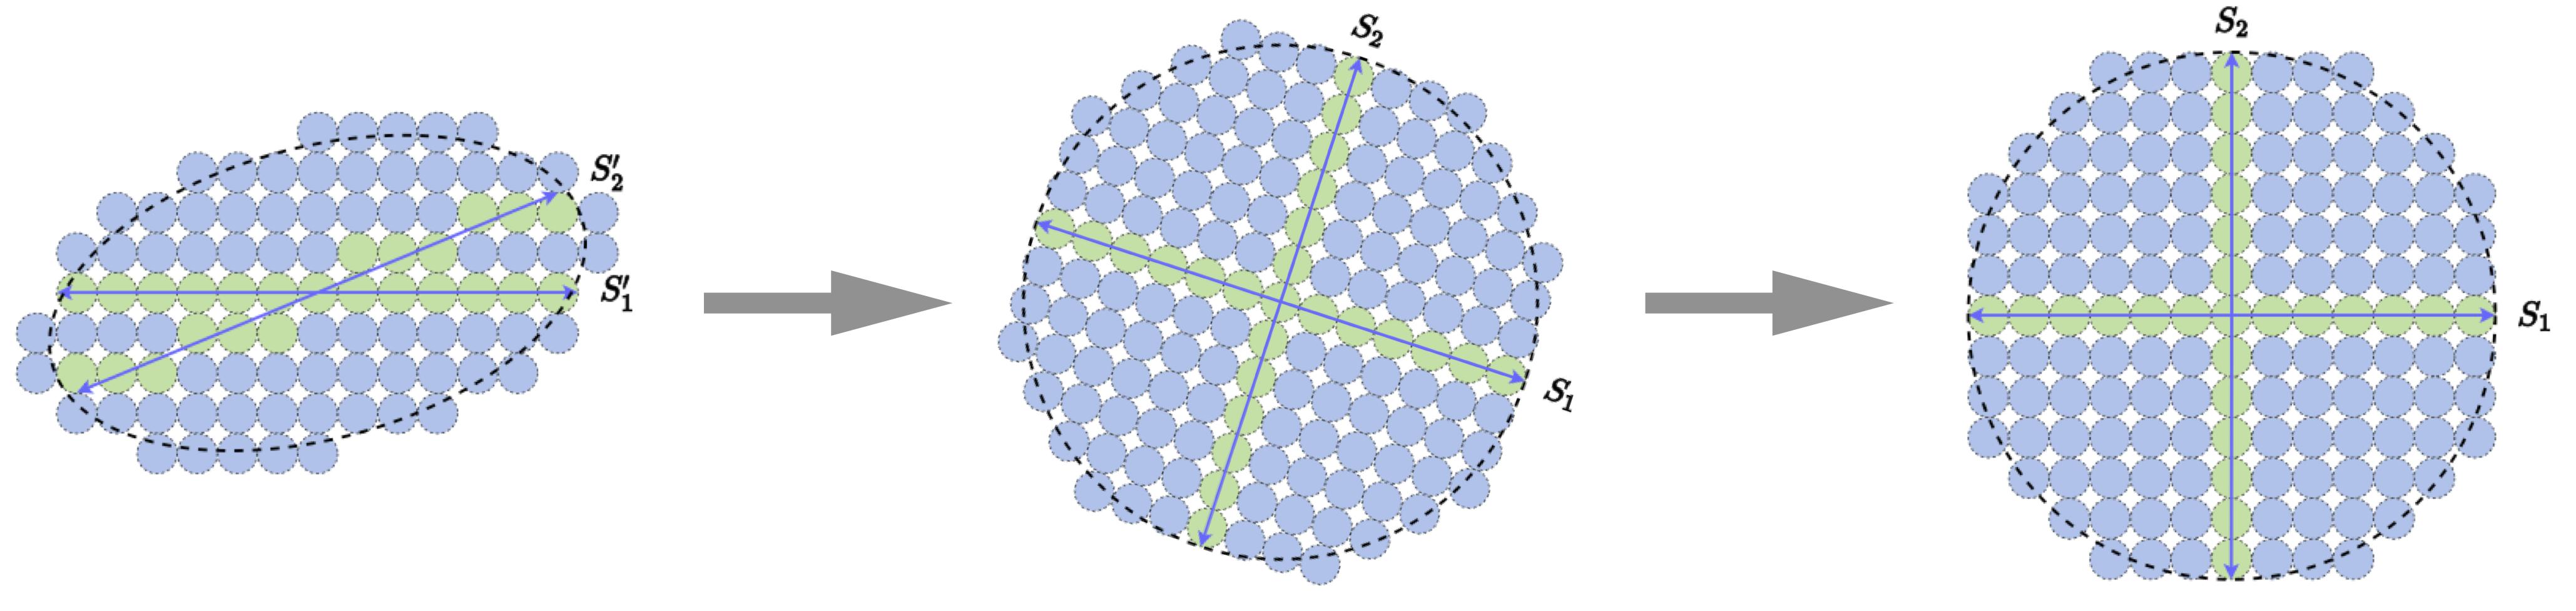
\includegraphics[width=0.95\textwidth]{\toplevelprefix/chapters/chapter4/figs/coding-transform.png}
    \caption{\small\textbf{Compararea a trei seturi de reprezentări prin reducerea ratei și raritate.} Fiecare $S_i$ reprezintă un subspațiu liniar, iar numărul de bile albastre reprezintă diferența dintre ratele de codare $\Delta R_{\epsilon}(\vZ \mid \vU_{[K]}) = R_\epsilon(\vZ) - R^c_\epsilon(\vZ \mid \vU_{[K]})$.}
    \label{fig:sparse-rate-reduction-diagram}
\end{figure}

\paragraph{Reducerea Ratei Rare.} Observăm că obiectivul de reducere a ratei \eqref{eq:rate reduction} este invariant la rotații arbitrare comune ale reprezentărilor și subspațiilor. În particular, optimizarea obiectivului de reducere a ratei poate să nu conducă în mod natural la reprezentări aliniate pe axe (adică, \textit{rare}). {De exemplu, considerați cele trei seturi de reprezentări învățate din \Cref{fig:sparse-rate-reduction-diagram}. Reducerea ratei de codare crește de la (a) la (b), dar deoarece este invariantă la rotații, rămâne aceeași de la (b) la (c).} Prin urmare, am dori să transformăm reprezentările (și subspațiile lor suport) astfel încât reprezentările $\vZ$ să devină în cele din urmă rare\footnote{Concret, având puține intrări nenule.} în raport cu coordonatele standard ale spațiului de reprezentare rezultat {ca în \Cref{fig:sparse-rate-reduction-diagram}(c)}. Prin urmare, pentru a ne asigura că reprezentările finale sunt potrivite pentru o codare mai compactă, am dori să transformăm reprezentările (și subspațiile lor suport) astfel încât să devină \textit{rare} în raport cu coordonatele standard ale spațiului de reprezentare rezultat.\footnote{Adică, având cele mai puține intrări nenule.} Computațional, putem combina cele două obiective de mai sus într-un obiectiv unificat pentru optimizare:
\begin{equation}
   \max_{f \in \mathcal{F}}\ [\Delta R_{\epsilon}(\Z \mid \vU_{[K]}) - \lambda \|\bm{Z}\|_0] \qquad \text{s.c.}\ \Z = f(\X),
   \label{eq:sparse-rr}
\end{equation}
unde $\mathcal{F}$ denotă o clasă generală de funcții și norma $\ell_0$ $\|\Z\|_0$ promovează raritatea reprezentărilor finale ale token-urilor \(\Z = f(\X)\).%


În practică, norma $\ell_0$ este adesea relaxată la norma $\ell_1$ pentru a îmbunătăți tractabilitatea computațională și a permite tehnici de optimizare convexă \cite{Wright-Ma-2022}. Motivați de aceasta, relaxăm Problema \eqref{eq:sparse-rr} în consecință, conducând la o formulare care rămâne fidelă obiectivului original de raritate, fiind în același timp mai potrivită pentru algoritmi eficienți, după cum urmează:
\begin{equation}
\begin{aligned}
   \max_{f \in \mathcal{F}}\ [\Delta R_{\epsilon}(\Z \mid \vU_{[K]}) - \lambda \|\bm{Z}\|_1]  \qquad \text{s.c.}\ \Z = f(\X),
   \label{eq:sparse-rr-1}
\end{aligned}
\end{equation}
Cu un ușor abuz de terminologie, ne referim adesea la această funcție obiectiv și ca \textit{reducere rară a ratei}.

\paragraph{Arhitectură de Rețea cu Cutie Albă prin Optimizare Desfășurată.}


Deși ușor de enunțat, fiecare termen din obiectivul de mai sus este provocator din punct de vedere computațional de optimizat \cite{Wright-Ma-2022}. Prin urmare, este natural să adoptăm o abordare de aproximare care realizează transformarea globală $f$ pentru a optimiza 
\eqref{eq:sparse-rr} printr-o concatenare a multiple, să zicem $L$, operațiuni simple \textit{incrementale și locale} $f^\ell$ care împing distribuția reprezentării către distribuția parsimonioasă dorită a modelului:
\begin{equation}
f\colon \X = \bm Z^0 \xrightarrow{\hspace{1mm} f^0 \hspace{1mm}} \Z^1 \rightarrow \cdots \rightarrow \Z^\ell \xrightarrow{\hspace{1mm} f^{\ell} \hspace{1mm}} \Z^{\ell+1} \rightarrow  \cdots \xrightarrow{\hspace{1mm} f^{L-1}} \Z^L = \Z,
\label{eq:incremental}
\end{equation}
unde $f^0: \bR^{D} \rightarrow \bR^{d}$ este maparea de pre-procesare care transformă fiecare token de intrare $\x_{i} \in \bR^{D}$ în reprezentările inițiale ale token-ului $\z_{i}^{1} \in \bR^{d}$.
Fiecare \textit{mapare directă} incrementală $\Z^{\ell + 1} = f^\ell(\Z^\ell)$, sau un „strat", transformă distribuția token-ului pentru a \textit{optimiza} obiectivul de reducere rară a ratei de mai sus \eqref{eq:sparse-rr}, condiționat de distribuția intrării sale $\Z^\ell$.

\begin{remark}
    În contrast cu alte abordări de optimizare desfășurată, cum ar fi ReduNet (vezi \Cref{sec:chap4-white-box-model-via-unrolling}), noi \textit{modelăm explicit} distribuția lui $\Z^\ell$ la fiecare strat, să zicem ca un amestec de subspații liniare sau generat rar dintr-un dicționar. Parametrii modelului sunt învățați din date (să zicem prin \textit{propagare înapoi} cu antrenament de la capăt la capăt). Această separare între „optimizarea" directă și
„învățarea" înapoi clarifică rolul matematic al fiecărui strat ca un operator
care transformă distribuția intrării sale, în timp ce distribuția de intrare este la rândul ei modelată (și ulterior învățată) de parametrii stratului.
\end{remark}

Acum, arătăm cum să derivăm aceste operațiuni incrementale și locale printr-o perspectivă de optimizare desfășurată pentru a rezolva Problema \eqref{eq:sparse-rr-1}. Odată ce decidem să folosim o abordare incrementală pentru optimizarea Problemei
\eqref{eq:sparse-rr-1}, există o varietate de alegeri posibile pentru a realiza optimizarea. Dat fiind un model pentru $\Z^\ell$, să zicem un amestec de subspații $\vU_{[K]}$, optăm pentru o metodă de \textit{minimizare alternantă} în doi pași cu o bază conceptuală puternică. Mai întâi, \textit{comprimăm} token-urile $\vZ^{\ell}$ printr-o coborâre pe gradient pentru a minimiza termenul ratei de codare $R^c_\epsilon (\vZ \mid \vU_{[K]}^\ell)$. Specific, facem un pas de gradient pe $R^c_\epsilon$ cu o rată de învățare $\kappa$ după cum urmează:
\begin{align}\label{eq:Z l+1/2}
    \bm Z^{\ell+1/2} = \bm Z^\ell - \kappa \nabla_{\bm Z} R^c_\epsilon (\vZ \mid \vU_{[K]}^\ell). 
\end{align}
Apoi, \textit{rarefiem} token-urile comprimate, generând \(\vZ^{\ell + 1}\) printr-un pas de gradient proximal relaxat corespunzător pentru a minimiza termenul rămas $\lambda \norm{\vZ}_{1} - R_{\epsilon}(\vZ)$. După cum vom argumenta în detaliu mai târziu, putem găsi un astfel de $\bm Z^{\ell+1}$ rezolvând o problemă de prezentare rară în raport cu un dicționar $\bm D^\ell$:
\begin{equation}\label{eq:Z l+1}
  \vZ^{\ell+1} = \argmin_{{\vZ}}  \bigg\{\lambda \norm{\vZ}_1 + \frac{1}{2}\norm{\vZ^{\ell + 1/2} - \vD^{\ell} {\vZ}}_F^2\bigg\}.
\end{equation}
În continuare, oferim detalii tehnice pentru fiecare dintre cei doi pași de mai sus și derivăm actualizări eficiente pentru implementarea lor.




\paragraph{Auto-Atenție ca Coborâre pe Gradient pe Rata de Codare a Reprezentărilor Token.} Pentru primul pas \eqref{eq:Z l+1/2}, gradientul ratei de codare \(\nabla_{\bm Z} R^c_\epsilon\) este costisitor de calculat, deoarece implică \(K\) inverse de matrice separate, câte una pentru fiecare dintre cele \(K\) subspații cu baza \(\vU_{k}^{\ell}\):
\begin{equation}
    \nabla_{\bm Z} R_{\epsilon}^c(\vZ \mid \vU_{[K]})
    = \frac{p}{N\epsilon^2}\sum_{k=1}^K \vU_k\vU_k^\top\vZ\Big(\I +
    \frac{p}{N\epsilon^2}(\vU_k^\top\vZ)^\top(\vU_k^\top\vZ)\Big)^{-1}.
    \label{eq:rate-gradient}
\end{equation}
Acum, demonstrăm că acest gradient poate fi aproximat în mod natural folosind un așa-numit operator de auto-atenție pe subspații multi-cap (MSSA), care are o formă funcțională similară cu operatorul de auto-atenție multi-cap \citep{vaswani2017attention} cu \(K\) capete (adică, unul pentru fiecare subspațiu, provenind din fiecare inversă de matrice). Aici, aproximăm gradientul \eqref{eq:rate-gradient} folosind seria Neumann de ordinul întâi (vezi \Cref{ex:neumannn}):
\begin{align}\label{eq:gd_rc_neumann}
    \nabla_{\bm Z} R_{\epsilon}^{c}(\vZ \mid \vU_{[K]}) 
    &\approx \frac{p}{N\epsilon^2} \sum_{k = 1}^{K}\vU_{k}\vU_{k}^\top\vZ\left(\vI - \frac{p}{N\epsilon^2} (\vU_{k}^\top\vZ)^\top(\vU_{k}^\top\vZ)\right) \notag \\
    &{= \frac{p}{N\epsilon^2} \left(\sum_{k = 1}^{K} \vU_{k}\vU_{k}^\top\right)\vZ -  \left( \frac{p}{N\epsilon^2}\right)^2\sum_{k = 1}^{K} \vU_{k}(\vU_{k}^\top\vZ)(\vU_{k}^\top\vZ)^\top(\vU_{k}^\top\vZ)}.
\end{align}
În această aproximare, calculăm similaritatea între reprezentările de token proiectate $\{\bm U_k^\top\bm z_i\}$ printr-o auto-corelație între caracteristicile proiectate ca $(\vU_{k}^\top\vZ)^\top(\vU_{k}^\top\vZ)$ și o convertim într-o distribuție de apartenență cu un softmax, și anume $\softmax{(\vU_{k}^\top\vZ)^\top(\vU_{k}^\top\vZ)}$.
Să presupunem că o uniune de subspații $\bm U_{[K]}$ acoperă întregul spațiu. Atunci, avem $\sum_{k = 1}^{K} \vU_{k}\vU_{k}^\top = \bm I$. Prin urmare, \eqref{eq:gd_rc_neumann} devine
\begin{align}\label{eq:grad Rc}
    \nabla_{\bm Z} R_{\epsilon}^{c}(\vZ \mid \vU_{[K]}) 
     \approx  \frac{p}{N\epsilon^2} \vZ -  \left( \frac{p}{N\epsilon^2}\right)^2 \MSSA\left(\vZ^{\ell} \mid \vU_{[K]}^{\ell}\right),
\end{align}
unde MSSA este definit printr-un operator SSA după cum urmează:
\begin{align}
    & \mathrm{SSA}\left(\vZ \mid \vU_{k}\right) 
    \doteq (\vU_{k}^\top \vZ)\mathrm{softmax}\left((\vU_{k}^\top\vZ)^\top(\vU_{k}^\top\vZ)\right), \ \forall k \in [K], \label{eq:SSA} \\
    & \mathrm{MSSA}\left(\vZ \mid \vU_{[K]}\right) 
    \doteq \frac{p}{N\epsilon^2} \mat{\vU_{1}, \dots, \vU_{K}}\mat{\mathrm{SSA}({\vZ \mid \vU_{1}}) \\ \vdots \\ \mathrm{SSA}({\vZ \mid \vU_{K}})}.\label{eq:Multi-Head-SSA}
\end{align}
Substituind \eqref{eq:grad Rc} în \eqref{eq:Z l+1/2} rezultă că poate fi aproximat în mod natural prin
\begin{equation}
    \vZ^{\ell + 1/2} = \left(1 - \frac{\kappa p}{N\epsilon^2}\right) \vZ^{\ell} + \frac{\kappa p}{N\epsilon^2} \mathrm{MSSA}\left(\vZ^{\ell}\ \middle|\ \vU_{[K]}^{\ell}\right).  \label{eq:gd-mcr-parts} 
\end{equation}



\begin{remark}
    Operatorul SSA din \eqref{eq:SSA} seamănă cu \textit{operatorul de atenție} dintr-un transformer tipic \citep{vaswani2017attention}, cu excepția că aici operatorii liniari de valoare, cheie și interogare sunt toți setați să fie \textit{aceiași} ca baza subspațiului, adică $\vV_{k} = \vK_{k} = \bm{Q}_{k} = \vU_k^*$. Prin urmare, numim $\mathrm{SSA}({\spcdot\mid\vU_k}): \bR^{d\times n} \rightarrow \bR^{p\times n}$ operatorul de \textbf{A}uto-\textbf{A}tenție pe \textbf{S}ubspații (SSA). Apoi, întregul operator MSSA din \eqref{eq:Multi-Head-SSA}, definit formal ca \(\mathrm{MSSA}({\spcdot \mid \vU_{[K]}}) \colon \bR^{d \times n} \to \bR^{d \times n}\) și numit operatorul de \textbf{A}uto-\textbf{A}tenție pe \textbf{S}ubspații \textbf{M}ulti-\textbf{C}ap (MSSA), agregă ieșirile capetelor de atenție prin medierea folosind ponderi dependente de model, similar în concept cu popularul operator de auto-atenție multi-cap din rețelele transformer existente. Pasul general de gradient \eqref{eq:gd-mcr-parts} seamănă cu auto-atenția multi-cap implementată cu o conexiune de salt în transformatoare.
\end{remark}




\paragraph{MLP ca Coborâre pe Gradient Proximal pentru Codarea Rară a Reprezentărilor Token.} Pentru al doilea pas al minimizării alternante, trebuie să minimizăm $\lambda \norm{\vZ}_{1} - R_{\epsilon}(\vZ)$. Observăm că gradientul \(\nabla R_{\epsilon}(\vZ)\) implică o inversă de matrice și, prin urmare, gradientul proximal naiv (vezi \Cref{subsec:pgd}) pentru a optimiza această problemă devine intractabil pentru probleme la scară largă. %
Prin urmare, adoptăm o abordare diferită, simplificatoare, pentru a face compromis între diversitatea reprezentațională și rarefiere: postulăm un dicționar (complet) incoerent sau ortogonal $\vD^{\ell} \in \bR^{d \times d}$ și cerem să rarefiem iterațiile intermediare $\vZ^{\ell + 1/2}$ în raport cu \(\vD^{\ell}\). Adică, $\vZ^{\ell + 1/2} \approx \vD^{\ell} \vZ^{\ell + 1}$ unde $\vZ^{\ell + 1}$ este mai rar; adică, este o \textit{codare rară} a lui \(\vZ^{\ell + 1/2}\). Dicționarul \(\vD^{\ell}\) este folosit pentru a rarefia toate token-urile simultan.
Prin ipoteza de incoerență, avem $(\vD^{\ell})^\top(\vD^{\ell}) \approx \vI$. Astfel din \eqref{eq:coding_rate} avem
\begin{equation}
    R_{\epsilon}(\vZ^{\ell + 1/2}) \approx R_{\epsilon}(\vD^{\ell}\vZ^{\ell + 1}) \approx R_{\epsilon}(\vZ^{\ell + 1}).
\end{equation}
Pentru a rezolva $\lambda \norm{\vZ}_{1} - R_{\epsilon}(\vZ)$, optimizăm următoarea problemă
\begin{align*}
       \vZ^{\ell + 1} \approx \argmin_{\vZ}  \norm{\vZ}_1 \quad \mbox{sub condiția} \quad \vZ^{\ell + 1/2} = \vD^{\ell}\vZ.
\end{align*}
{Programul de reprezentare rară de mai sus este de obicei rezolvat prin relaxarea lui la un program convex neconstrâns, cunoscut ca LASSO \citep{Wright-Ma-2022}:}
\begin{equation}
    \vZ^{\ell + 1} \approx \argmin_{\vZ} \left[\lambda \norm{\vZ}_1 + \frac{1}{2}\norm{\vZ^{\ell + 1/2} - \vD^{\ell} \vZ}_F^2 \right].
\end{equation}
În implementarea noastră, adăugăm și o constrângere nenegativă la $\vZ^{\ell + 1}$ și rezolvăm LASSO nenegativ corespunzător:
\begin{equation}
    \vZ^{\ell + 1} \approx \argmin_{\vZ \geq \bm 0} \left[\lambda\norm{\vZ}_1 + \frac{1}{2}\norm{\vZ^{\ell + 1/2} - \vD^{\ell} \vZ}_{F}^{2}\right].
    \label{eq:sparse-nonnegative}
\end{equation}
Apoi, optimizăm incremental \Cref{eq:sparse-nonnegative} efectuând un pas de {\em coborâre pe gradient proximal} desfășurat, cunoscut ca un pas ISTA \citep{beck2009fast}, pentru a da actualizarea:
\begin{align}\label{eq:ista-block}
    \vZ^{\ell + 1} 
    &= \mathrm{ISTA}({\vZ^{\ell + 1/2} \mid \vD^{\ell}}), \\
    \text{unde} \quad \mathrm{ISTA}({\vZ \mid \vD}) 
    &\doteq \operatorname{ReLU}(\vZ - \eta \vD^\top(\vD\vZ - \vZ) - \eta \lambda \bm{1}).
\end{align}






\begin{figure}
     \centering
     \includegraphics[width=0.75\textwidth]{\toplevelprefix/chapters/chapter4/figs/crate_encoder_architecture.pdf}
    \caption{\small \textbf{Un strat al arhitecturii encoder CRATE.} Arhitectura completă este pur și simplu o concatenare a unor astfel de straturi, cu un tokenizator inițial, un cap de pre-procesare și un cap final specific sarcinii (adică, un cap de clasificare).}
    \label{fig:crate_backbone}
\end{figure}



\subsection{Arhitectura Generală de Transformer cu Cutie Albă: CRATE}

Acum proiectăm o arhitectură de transformer cu cutie albă, numită Transformatorul RATE de Codare (\textsc{crate}), prin desfășurarea actualizărilor de mai sus. Combinând cei doi pași de mai sus \eqref{eq:gd-mcr-parts} și \eqref{eq:ista-block}:
\begin{enumerate}[leftmargin=0.7cm]
    \item Compresia locală a token-urilor într-un eșantion către o structură de amestec de subspații, conducând la blocul de auto-atenție pe subspații multi-cap -- \texttt{MSSA};
    \item Rarefierea globală a seturilor de token-uri pe toate eșantioanele prin codare rară, conducând la blocul de rarefiere -- \texttt{ISTA};
\end{enumerate}
putem obține următorul strat de transformer bazat pe reducerea ratei, ilustrat în \Cref{fig:crate_backbone},
\begin{equation}
    \vZ^{\ell+1/2} \doteq \vZ^{\ell} + \texttt{MSSA}(\vZ^{\ell} \mid \vU_{[K]}^{\ell}), 
    \qquad 
    \vZ^{\ell+1}\doteq \texttt{ISTA}(\vZ^{\ell+1/2} \mid \bm D^\ell).
\end{equation}
Compunând mai multe astfel de straturi urmând construcția incrementală a reprezentării noastre din \eqref{eq:incremental}, obținem o arhitectură de transformer cu cutie albă care transformă token-urile de date către o uniune compactă și rară de subspații incoerente, unde $f^{\pre}: \bR^{D \times N} \rightarrow \bR^{d \times N}$ este maparea de pre-procesare care transformă token-urile de intrare $\vX \in \bR^{D \times N}$ în reprezentări de prim strat $\vZ^{1} \in \bR^{d \times N}$. Un flux general al acestei arhitecturi a fost arătat în \Cref{fig:crate-diagram}.

\begin{figure}[t!]
     \centering
         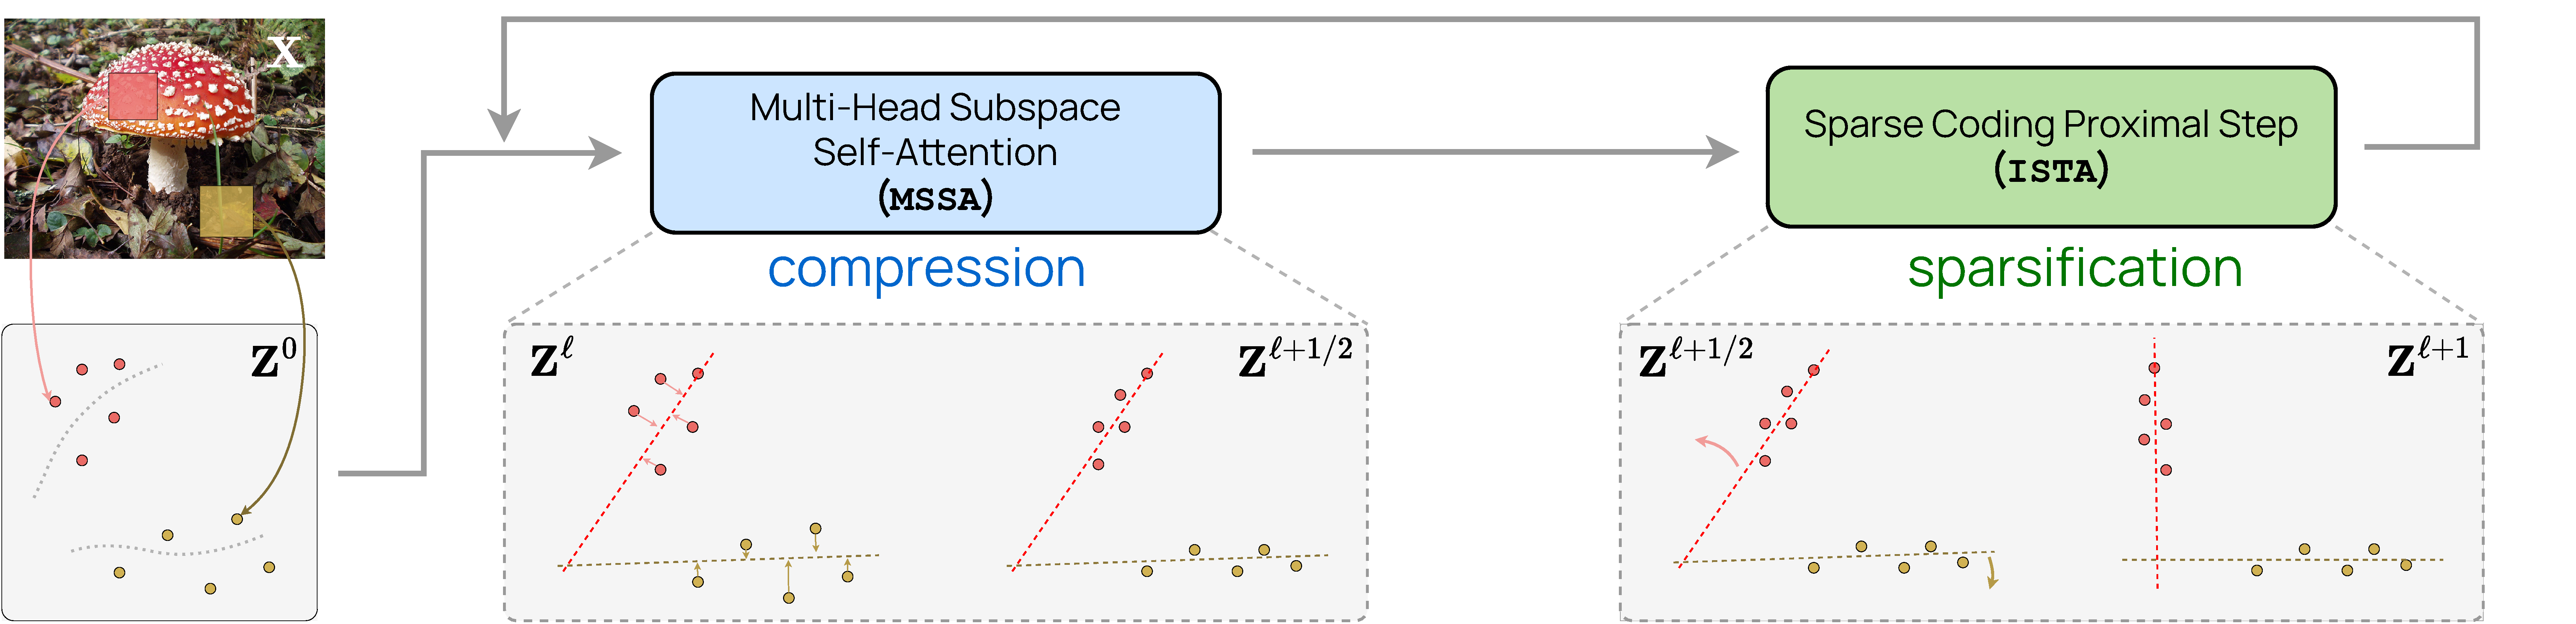
\includegraphics[width=\textwidth]{\toplevelprefix/chapters/chapter4/figs/CRATE_fig1_patches.pdf}
     \vspace{-0.1in}
     \caption{
     \textbf{„Bucla principală" a proiectării rețelei profunde cu cutie albă \textsc{crate}.}
     După codarea datelor de intrare ca o secvență de token-uri $\vZ^0$, \textsc{crate} construiește o rețea profundă care transformă datele într-o configurație canonică de subspații de dimensiune mică prin {\textit{\textbf{compresie}}} succesivă
     împotriva unui model local pentru distribuție, generând $\vZ^{\ell+1/2}$, și {\textit{\textbf{rarefiere}}}
     împotriva unui dicționar global, generând $\vZ^{\ell+1}$.
     Stivuirea repetată a acestor blocuri și antrenarea parametrilor modelului prin propagare înapoi produce o reprezentare puternică și interpretabilă a datelor.
     }
        \label{fig:crate-diagram}
\end{figure}


\begin{remark}[\textbf{Rolurile pasului înainte și propagării înapoi}]\label{sub:forward_backward}
    În contrast cu alte abordări de optimizare desfășurată, cum ar fi ReduNet \cite{chan2021redunet}, noi \textit{modelăm explicit} distribuția fiecărui $\vZ^\ell$ și $\vZ^{\ell + 1/2}$ la fiecare strat, fie printr-un amestec de subspații liniare, fie generat rar dintr-un dicționar. Am introdus interpretarea că la fiecare strat \(\ell\), bazele învățate pentru subspații \(\vU_{[K]}^{\ell}\) și dicționarele învățate \(\vD^{\ell}\) servesc împreună ca un \textit{codebook} sau \textit{filtru de analiză} care codifică și transformă reprezentările intermediare la fiecare strat \(\ell\). Deoarece distribuția de intrare la stratul \(\ell\) este mai întâi modelată de \(\vU_{[K]}^{\ell}\) apoi transformată de \(\vD^{\ell}\), distribuția de intrare la fiecare strat este diferită și astfel necesităm un codebook separat la fiecare strat pentru a obține cea mai parsimonioasă codare. Parametrii acestor codebook-uri (adică bazele subspațiilor și dicționarele), presupuși până acum ca fiind perfect cunoscuți, sunt de fapt învățați din date (să zicem prin \textit{propagare înapoi} în cadrul antrenării de la capăt la capăt).
    
    Prin urmare, metodologia noastră prezintă o separare conceptuală clară între „optimizarea" directă și „învățarea" înapoi pentru rețeaua neuronală profundă cu cutie albă astfel derivată. Și anume, în pasul său înainte, interpretăm fiecare strat ca un operator care, condiționat de un model învățat (adică un codebook) pentru distribuția intrării sale, transformă această distribuție către o reprezentare mai parsimonioasă. În propagarea sa înapoi, codebook-ul acestui model, pentru distribuția intrării la fiecare strat, este actualizat pentru a se potrivi mai bine unei anumite relații (supervizate) intrare-ieșire, așa cum este ilustrat în \Cref{fig:forward-backward}. Această interpretare conceptuală implică un anumit agnosticism al reprezentărilor modelului față de sarcina și pierderea particulare; în special, multe tipuri de sarcini și pierderi vor asigura că modelele la fiecare strat sunt potrivite, ceea ce asigură că modelul produce reprezentări parsimonioase.
\end{remark}






Acum prezentăm performanța empirică a rețelelor propuse \textsc{crate} măsurând acuratețea lor de clasificare top-1 pe ImageNet-1K, precum și performanța de învățare prin transfer pe mai multe seturi de date downstream utilizate pe scară largă.
Rezumăm rezultatele în \Cref{tab:crate_comparison_with_sota}. Metodologia de învățare prin transfer este de a face ajustare fină folosind pierderea de entropie încrucișată inițializând din rețelele pre-antrenate.
Deoarece arhitectura de transformer cu cutie albă proiectată folosește partajarea parametrilor atât în blocul de atenție (\texttt{MSSA}) cât și în blocul de neliniaritate (\texttt{ISTA}), modelul \textsc{crate}{-Base} (22,80 milioane)
are un număr similar de parametri cu ViT-Small (22,05 milioane)~\cite{dosovitskiy2020image} și mai puțin de 30% din parametrii unui ViT-Base configurat identic (86,54 milioane).
Din \Cref{tab:crate_comparison_with_sota}, constatăm că, cu un număr similar de parametri ai modelului, rețeaua noastră propusă obține performanțe similare pe ImageNet-1K și de învățare prin transfer ca ViT, având în același timp un design simplu și principial. Mai mult, cu același set de hiperparametri de antrenare, observăm un comportament promițător de scalare în \textsc{crate}---îmbunătățim în mod constant performanța prin creșterea dimensiunii modelului. Pentru a rezuma, \textsc{crate} obține performanțe promițătoare pe seturi de date la scară largă din lumea reală prin implementarea directă a arhitecturii noastre principiale. Vom oferi mai multe detalii despre implementare și analiza rezultatelor experimentale privind clasificarea imaginilor în aplicația finală \Cref{ch:applications}.

\begin{figure}[t]
    \begin{subfigure}[t]{0.48\textwidth}
        \centering
        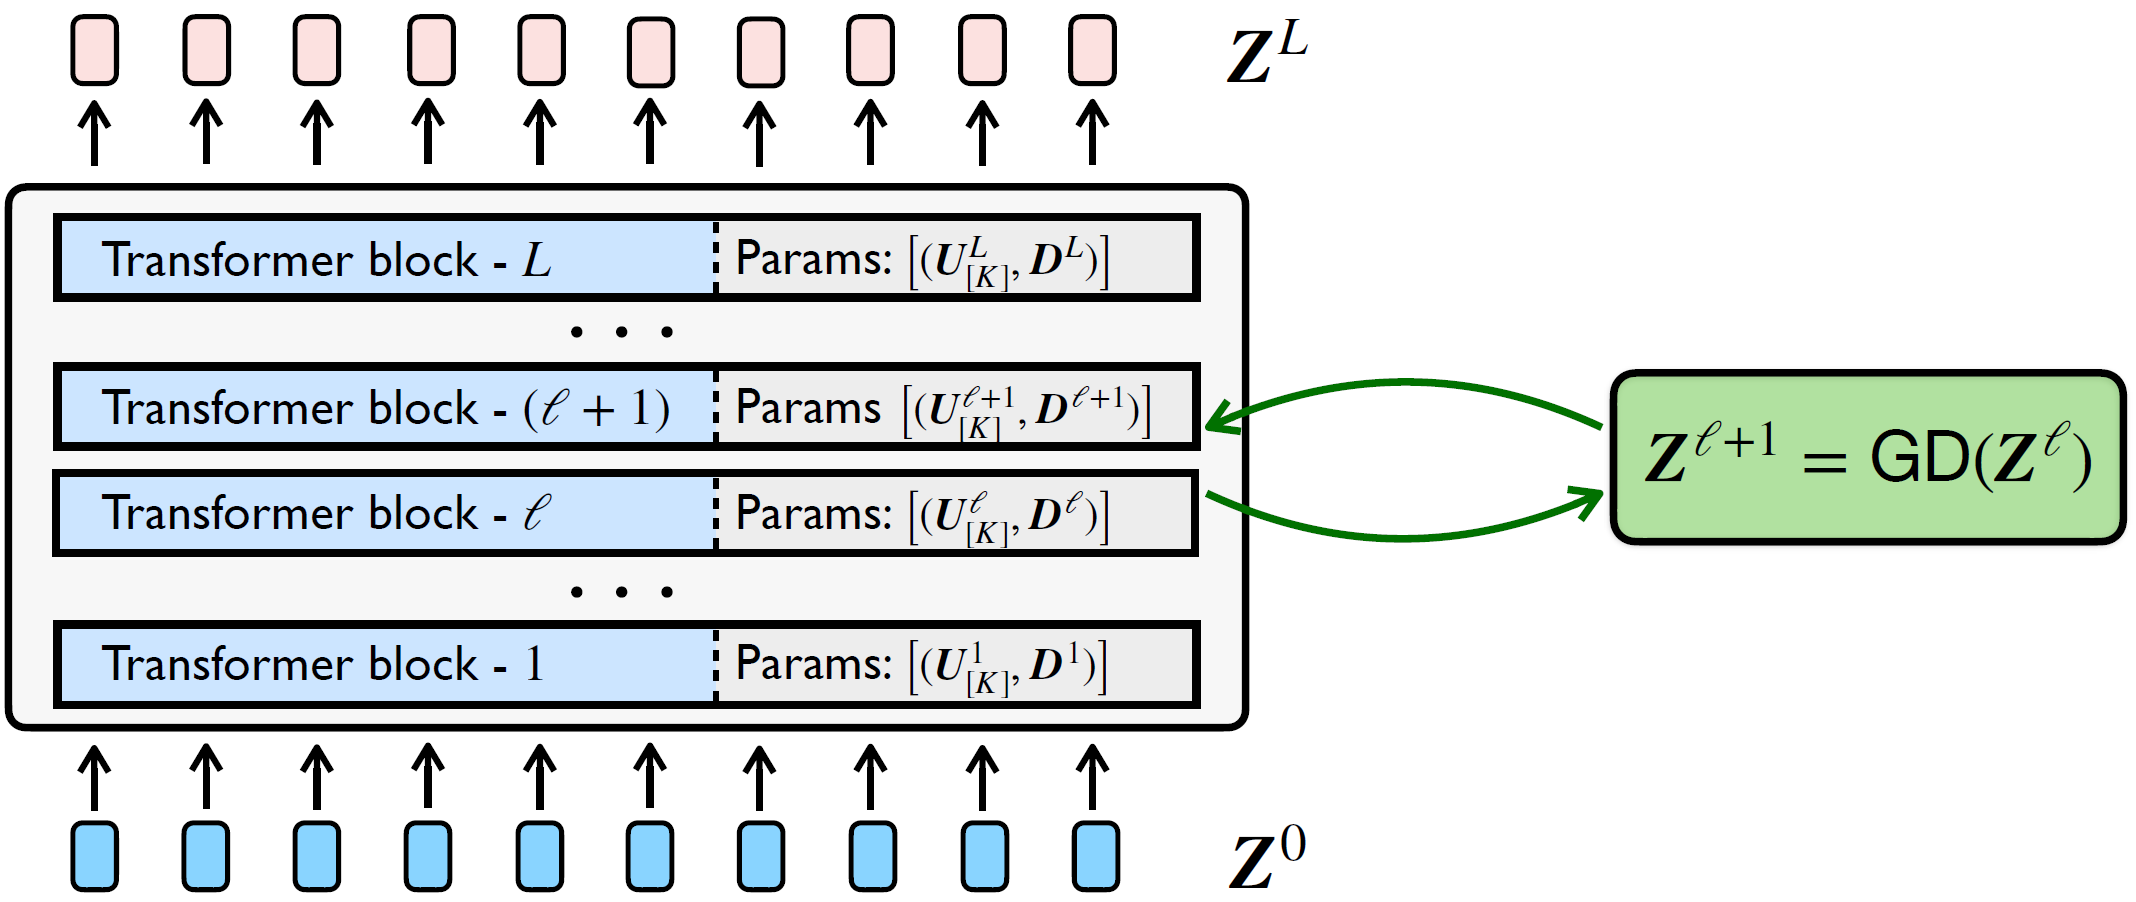
\includegraphics[width=\textwidth]{\toplevelprefix/chapters/chapter4/figs/forward.png}
        \caption{\bf Pasul înainte}
    \end{subfigure}
    \hfill
    \begin{subfigure}[t]{0.48\textwidth}
        \centering
        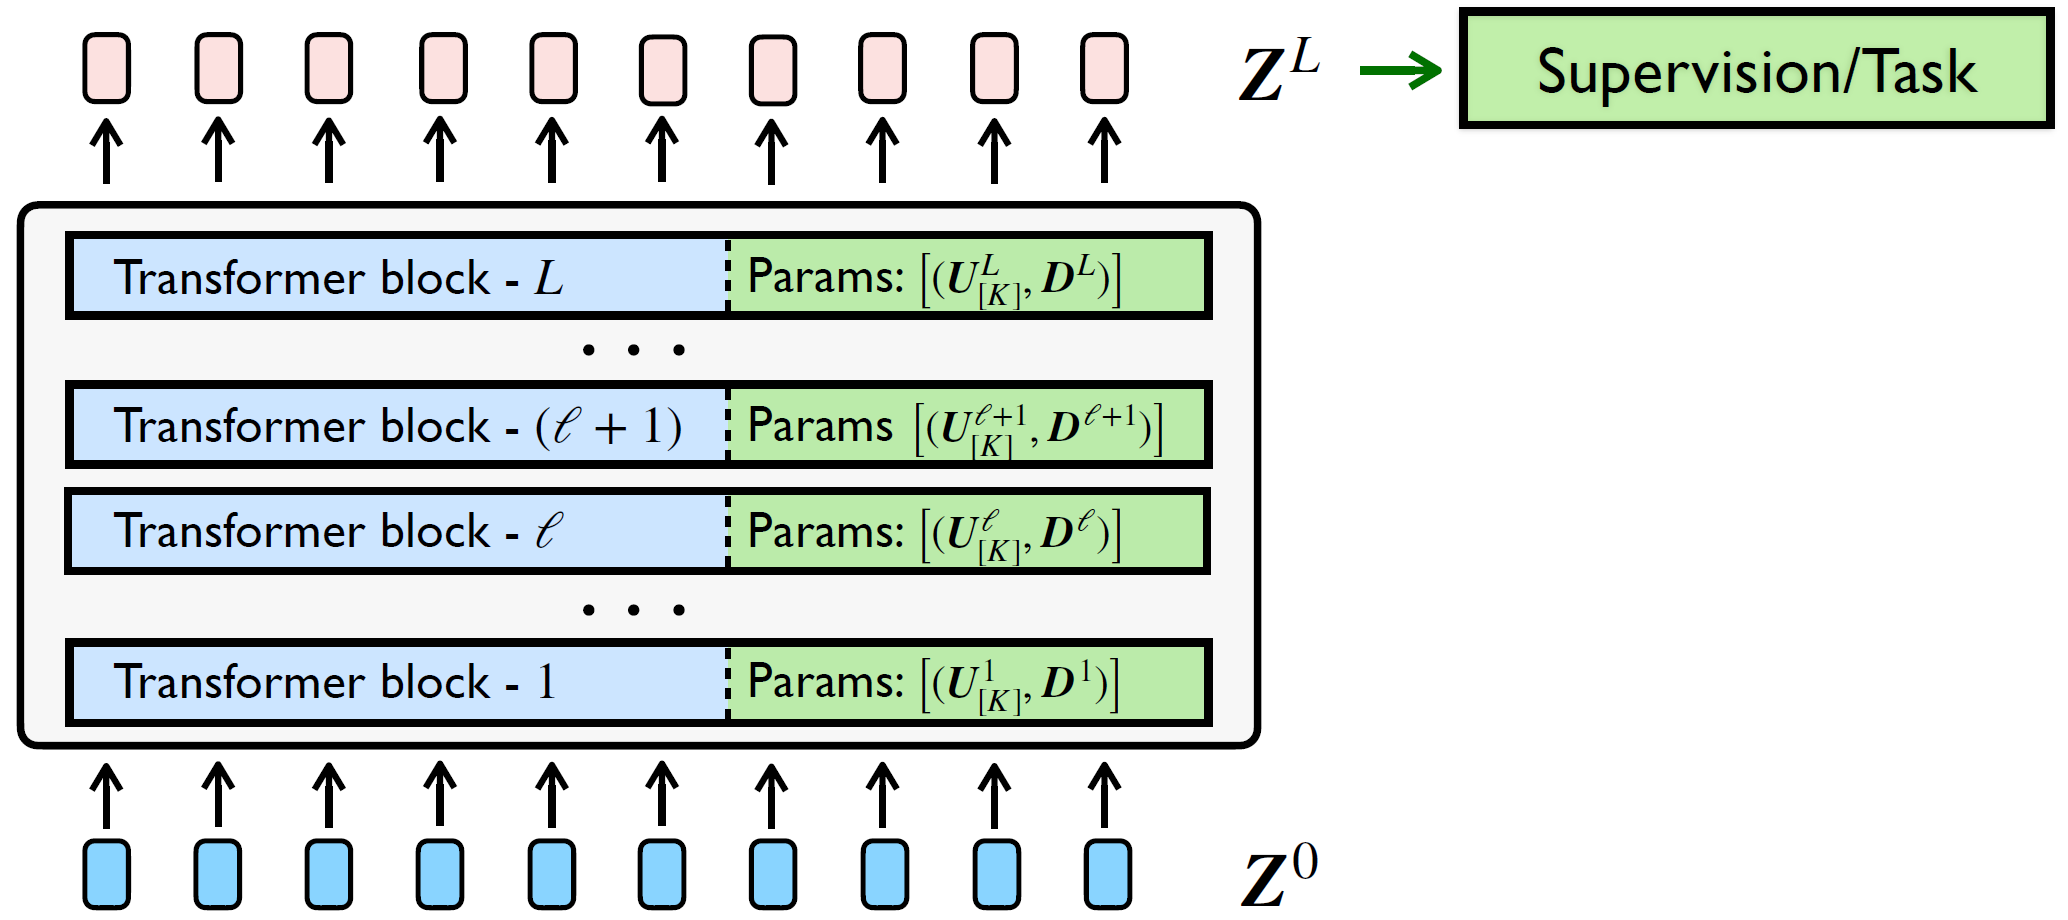
\includegraphics[width=\textwidth]{\toplevelprefix/chapters/chapter4/figs/backward.png}
        \caption{\bf Propagarea înapoi}
    \end{subfigure}
    \caption{\small {\bf Rolurile pasului înainte și propagării înapoi în rețelele profunde}. (a) Date fiind subspații și dicționare fixe $\{(\bm U_{[K]}^{\ell}, \bm D^{\ell})\}_{\ell=1}^L$, fiecare strat efectuează compresie și rarefiere asupra reprezentărilor în pasul înainte; (b) Propagarea înapoi învață subspații și dicționare $\{(\bm U_{[K]}^{\ell}, \bm D^{\ell})\}_{\ell=1}^L$ din datele de antrenare.}
    \label{fig:forward-backward}
\end{figure}


\begin{table*}[t!]
\centering
\caption{\small Acuratețea de clasificare top-1 a \textsc{crate} pe diferite seturi de date cu diferite scale de model
când este pre-antrenat pe ImageNet-1K. Pentru ImageNet-1K/ImageNet-1K ReaL, evaluăm direct acuratețea top-1. Pentru alte seturi de date, folosim modele care sunt pre-antrenate pe ImageNet ca inițializare și evaluăm performanța de învățare prin transfer prin ajustare fină.}
\label{tab:crate_comparison_with_sota}
\small
    \setlength{\tabcolsep}{13.6pt}
\resizebox{0.98\textwidth}{!}{\begin{tabular}{@{}lcccc|cc@{}}
\toprule
\textbf{Model} & \textsc{crate}{-T}  &  \textsc{crate}{-S} & \textsc{crate}{-B} & \textsc{crate}{-L} & { \color{gray} ViT-T} &  { \color{gray}ViT-S } \\ 
\midrule
\midrule
 \# parametri & 6,09M & 13,12M & 22,80M & 77,64M & { \color{gray} 5,72M} & { \color{gray} 22,05M} \\
\midrule
 ImageNet-1K & 66,7 & 69,2 & 70,8 & 71,3 & { \color{gray} 71,5} & { \color{gray} 72,4} \\
 ImageNet-1K ReaL & 74,0 & 76,0 & 76,5 & 77,4 & { \color{gray} 78,3 } & { \color{gray} 78,4} \\
 \midrule
 CIFAR10 & 95,5 & 96,0 & 96,8 & 97,2 & { \color{gray} 96,6} & { \color{gray} 97,2} \\
 CIFAR100 & 78,9 & 81,0 & 82,7 & 83,6 & { \color{gray} 81,8} & { \color{gray} 83,2}\\
 Oxford Flowers-102 & 84,6 & 87,1 & 88,7 & 88,3 & { \color{gray} 85,1} & { \color{gray} 88,5}\\
 Oxford-IIIT-Pets & 81,4 & 84,9 & 85,3 & 87,4 & { \color{gray} 88,5} & { \color{gray} 88,6} \\
 \bottomrule
\end{tabular}}
\end{table*}



\section{Variante de Arhitecturi Profunde prin Design} \label{sec:chap4-derive-white-box-transformer-variants}

Până acum, sperăm că am oferit dovezi convingătoare că rolul rețelelor profunde (populare) este de a realiza anumite algoritmi de optimizare pentru minimizarea ratei de codare (sau maximizarea câștigului de informație) a reprezentărilor învățate. Cu toate acestea, cititorii care sunt familiarizați cu metodele de optimizare ar fi putut observa că arhitecturile de mai sus (ReduNet sau CRATE) corespund unor tehnici de optimizare destul de de bază. Ele ar putea avea mult spațiu pentru îmbunătățire în eficiență sau eficacitate. Mai mult, dacă credem că cadrul teoretic propus pentru interpretarea rețelelor profunde este corect, acesta nu ar trebui doar să ajute la explicarea arhitecturilor existente, ci ar trebui să ne ghideze în dezvoltarea unor arhitecturi mai eficiente și eficace. În această secțiune, arătăm că acest lucru ar putea fi cazul: noile arhitecturi rezultate nu sunt doar complet interpretabile, ci și cu corectitudine garantată și eficiență îmbunătățită.




\subsection{Arhitectură de Transformer Doar cu Atenție} \label{sub:aot}

În această subsecțiune, propunem o arhitectură minimalistă de transformer constând din straturi interpretabile bazate pe operatorul MSSA. Pentru a deriva o arhitectură de transformer complet interpretabilă cu doar componentele necesare,
susținem că obiectivul învățării reprezentării este de a comprima un set de reprezentări inițiale zgomotoase ale token-urilor către un amestec de subspații de dimensiune mică. %
Aici, presupunem că reprezentările inițiale ale token-urilor $\bm Z^{(1)}$ sunt eșantionate dintr-un amestec de gaussiene de rang mic perturbate de zgomot după cum urmează:
\begin{definition}\label{def:MoG}
Fie $C_1,\dots,C_K$ o partiție a setului de indici $[N]$ și $\bm U_k \in \mathcal{O}^{d \times p_k}$ să denoteze baza ortonormală a celui de-al $k$-lea subspațiu pentru fiecare $k \in [K]$. Spunem că reprezentările token-urilor $\{\bm z_i \}_{i=1}^N \subseteq \R^d$ sunt eșantionate dintr-un amestec de distribuții gaussiene zgomotoase de rang mic dacă pentru fiecare $k \in [K]$,
\begin{align}\label{eq:MoG}
    \bm z_i = \underbrace{\bm U_{k} \bm a_i}_{\bf semnal} + \underbrace{\sum_{j \neq k}^K \bm U_j \bm e_{i,j}}_{\bf zgomot},\ \forall i \in C_k, 
\end{align}
unde $\bm{a}_i \overset{i.i.d.}{\sim} \mathcal{N}(\bm{0},\bm{I}_{p_k})$ și $\bm{e}_{i,j} \overset{i.i.d.}{\sim} \mathcal{N}(\bm{0},\delta^2\bm{I}_{p_j})$ pentru toți $i \in C_k$ și $k \in [K]$, $\{\bm{a}_i\}$ și $\{\bm{e}_{i,j}\}$ sunt respectiv mutual independente, și $\{\bm{a}_i\}$ este independent de $\{\bm{e}_{i,j}\}$.
\end{definition}
Acest model servește ca un cadru idealizat pentru aproximarea reprezentărilor token-urilor în LLM-urile pre-antrenate din lumea reală. Acesta presupune că reprezentările token-urilor sunt eșantionate dintr-un amestec de distribuții gaussiene multiple de rang mic cu zgomot. În plus, acest model se aliniază bine cu două ipoteze bine stabilite despre structura reprezentărilor token-urilor în modelele de limbaj mari pre-antrenate: „ipoteza reprezentării liniare" \citep{jiang2024origins,park2023linear} și „ipoteza suprapunerii" \citep{elhage2022toy,yun2021transformer}.

\begin{remark}
    Ipoteza reprezentării liniare postulează că reprezentările token-urilor în LLM-uri se află în subspații liniare de dimensiune mică care codifică caracteristici semantice. Similar, ipoteza suprapunerii sugerează că aceste reprezentări pot fi exprimate aproximativ ca o combinație liniară rară a acestor vectori de caracteristici. În \Cref{def:MoG}, fiecare bază $\bm U_k$ a subspațiilor poate fi interpretată ca un set de caracteristici semantice, unde fiecare caracteristică corespunde unui aspect specific al sensului token-ului. Reprezentările token-urilor sunt apoi exprimate aproximativ ca combinații liniare rare ale acestor baze de subspații, capturând componentele semantice esențiale ale token-ului în timp ce ignoră dimensiunile irelevante.
\end{remark}

\paragraph{Operator de Eliminare a Zgomotului pentru Reprezentările Token.} Acum, arătăm că operatorul MSSA (vezi \eqref{eq:Multi-Head-SSA}) poate elimina incremental zgomotul din reprezentările token-urilor generate din modelul de mai sus. Specific, considerăm pentru fiecare $\ell =1 ,\dots,L$,
\begin{align}\label{eq:MSSA}
    \bm Z^{(\ell+1)} =  \bm Z^{(\ell)} + \eta \sum_{k=1}^K \bm U_k\bm U_k^T \bm Z^{(\ell)} \varphi \left(\bm Z^{(\ell)^T}\bm U_k\bm U_k^T\bm Z^{(\ell)} \right),
\end{align}
unde $\{\bm U_k\}_{k=1}^K$ este definit în \Cref{def:MoG}, $\eta > 0$ este dimensiunea pasului, și $\varphi$ este un operator element cu element, cum ar fi softmax, ReLU, sau alte funcții. Pentru a simplifica dezvoltarea noastră, presupunem că subspațiile din \Cref{def:MoG} sunt ortogonale între ele, adică $\bm U_k^T\bm U_j = \bm 0$ pentru toți $k \neq j$. Observăm că această presupunere nu este restrictivă, deoarece în spații cu dimensiune mare, subspațiile aleatoare de dimensiune mică sunt incoerente între ele cu probabilitate mare, adică $\bm U_k^T\bm U_j \approx \bm 0$ \citep{Wright-Ma-2021}.\footnote{Se poate generaliza direct rezultatele noastre la subspații ne-ortogonale, cu o analiză ușor mai sofisticată.}

\begin{figure}[t]
    \begin{subfigure}[t]{0.45\textwidth}
        \centering
        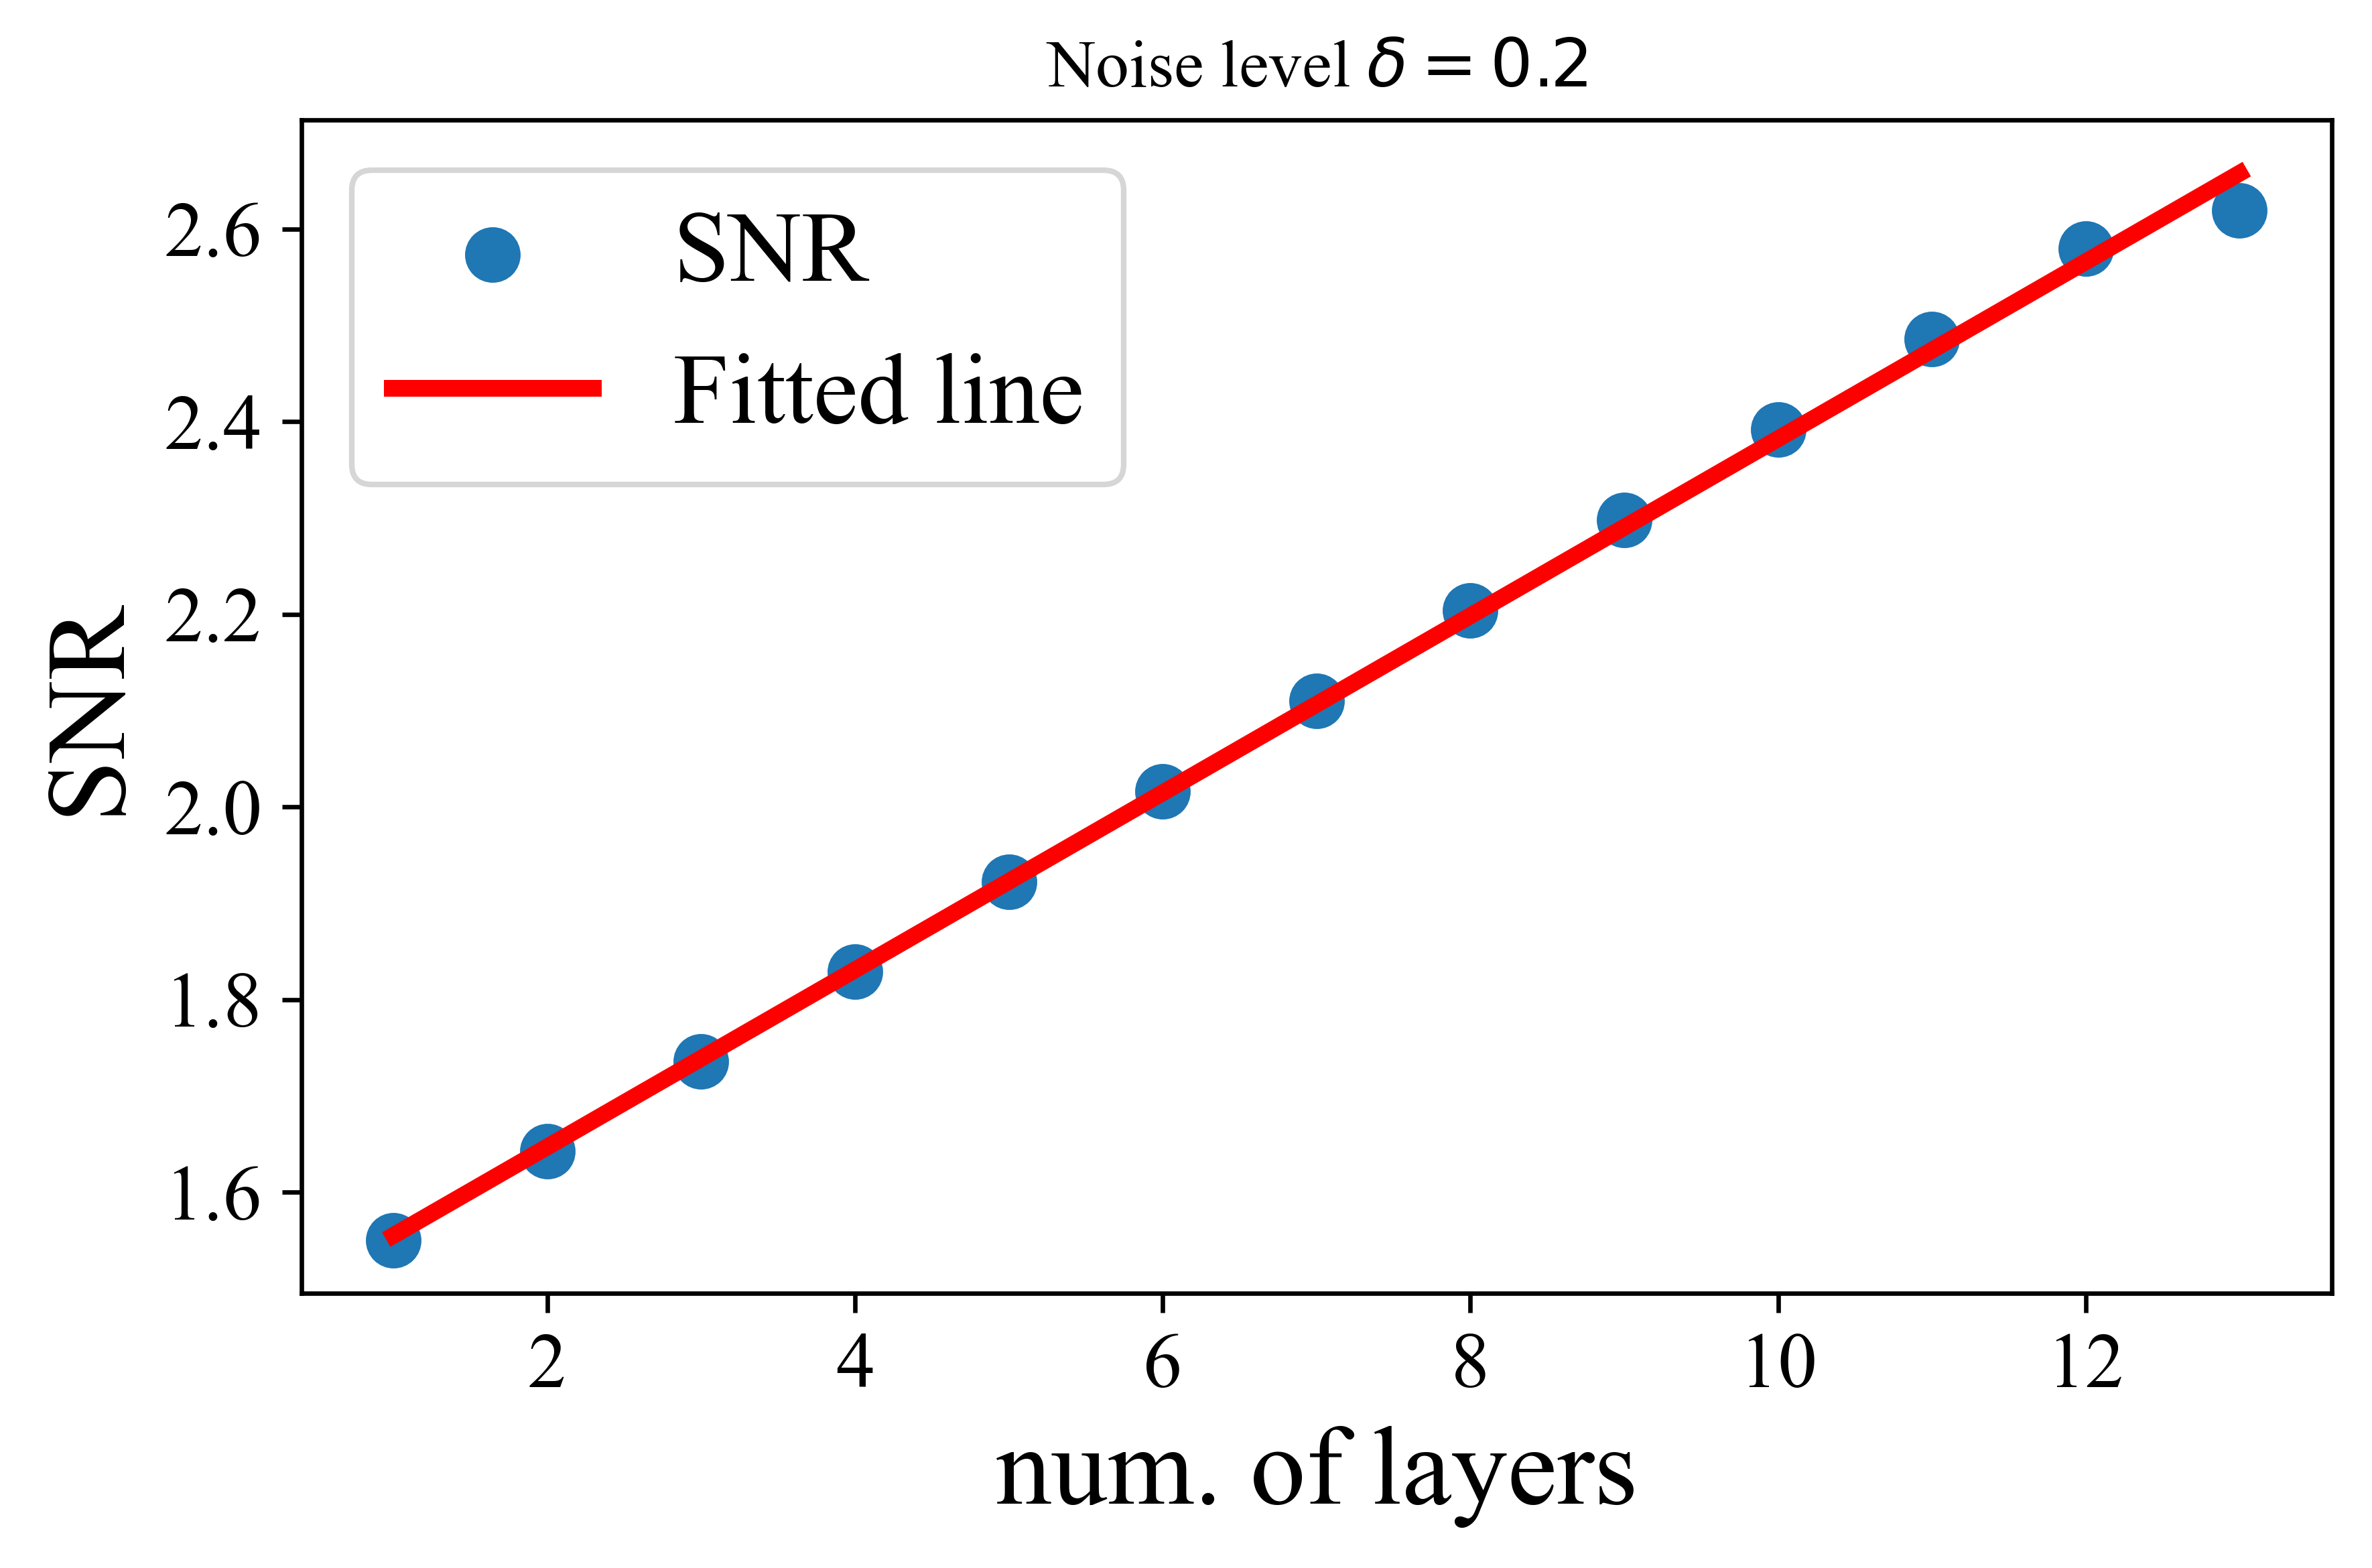
\includegraphics[width=\textwidth]{\toplevelprefix/chapters/chapter4/figs/SNR1.png}
        \caption{Nivel de zgomot $\delta = 0,2$}
    \end{subfigure}
    \hfill
    \begin{subfigure}[t]{0.45\textwidth}
        \centering
        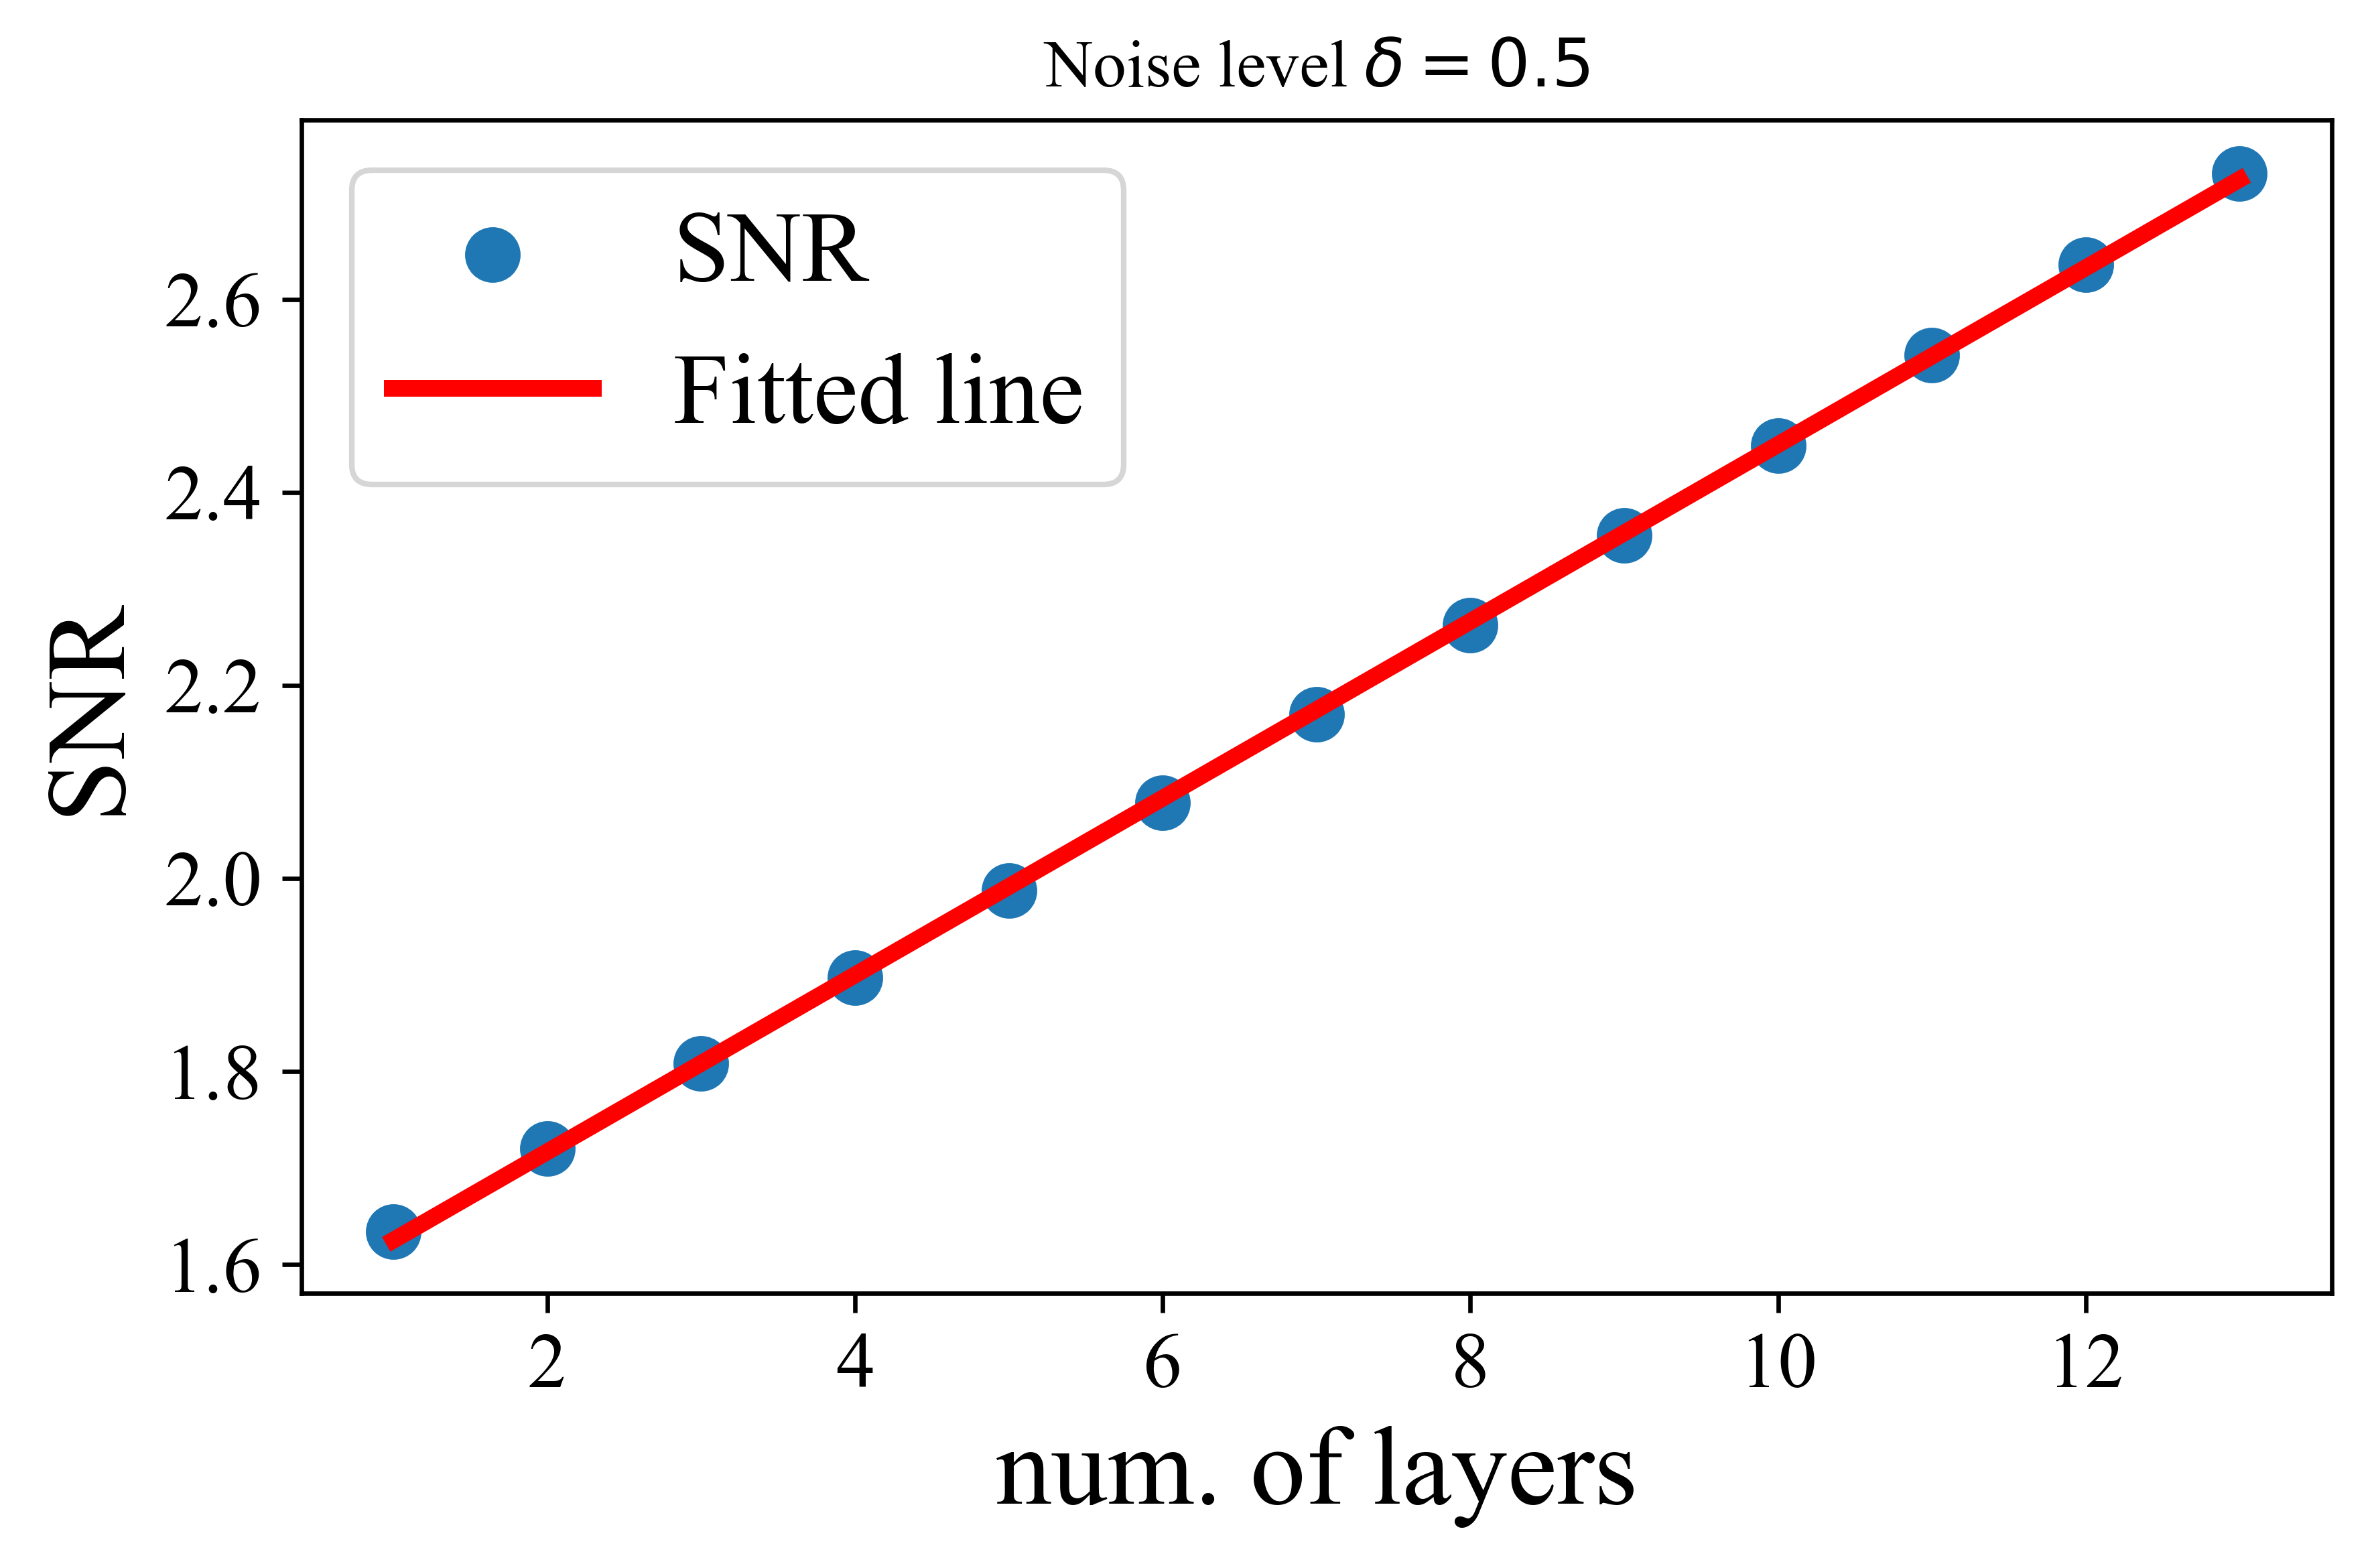
\includegraphics[width=\textwidth]{\toplevelprefix/chapters/chapter4/figs/SNR2.png}
        \caption{Nivel de zgomot $\delta = 0,5$}
    \end{subfigure}
    \caption{{\bf Performanța de eliminare a zgomotului a transformatorului doar cu atenție.} Aici, eșantionăm reprezentări inițiale ale token-urilor dintr-un amestec de gaussiene de rang mic din \Cref{def:MoG}. Apoi, aplicăm \eqref{eq:MSSA} pentru a actualiza reprezentările token-urilor și raportăm SNR-ul la fiecare strat.} \label{fig:MSSA}
\end{figure}


Acum, fie coloanele lui $\bm Z_k^{(\ell)}$ să denoteze reprezentările token-urilor din al $k$-lea subspațiu la al $\ell$-lea strat. Pentru a cuantifica capacitatea de eliminare a zgomotului, definim raportul semnal-zgomot (SNR) pentru fiecare bloc al reprezentărilor token-urilor la al $\ell$-lea strat după cum urmează:
\begin{align}\label{def:SNR}
\mathrm{SNR}(\bm Z_k^{(\ell)}) \doteq  \frac{\|\bm U_k\bm U_k^T\bm Z_k^{(\ell)} \|_F}{\|(\bm I - \bm U_k\bm U_k^T)\bm Z_k^{(\ell)} \|_F},\quad \forall k \in [K].
\end{align}
Pentru a simplifica analiza noastră, presupunem că $p=p_1=\dots=p_K$, $N_1=\dots=N_K=N/K$, și
\begin{align}\label{eq:orth}
\begin{bmatrix}
\bm U_1 & \dots & \bm U_K
\end{bmatrix} \in \mathcal{O}^{d\times Kp}.
\end{align}

Cu configurația de mai sus, acum caracterizăm performanța de eliminare a zgomotului a operatorului MSSA.

\begin{figure*}[t]
\begin{center}
        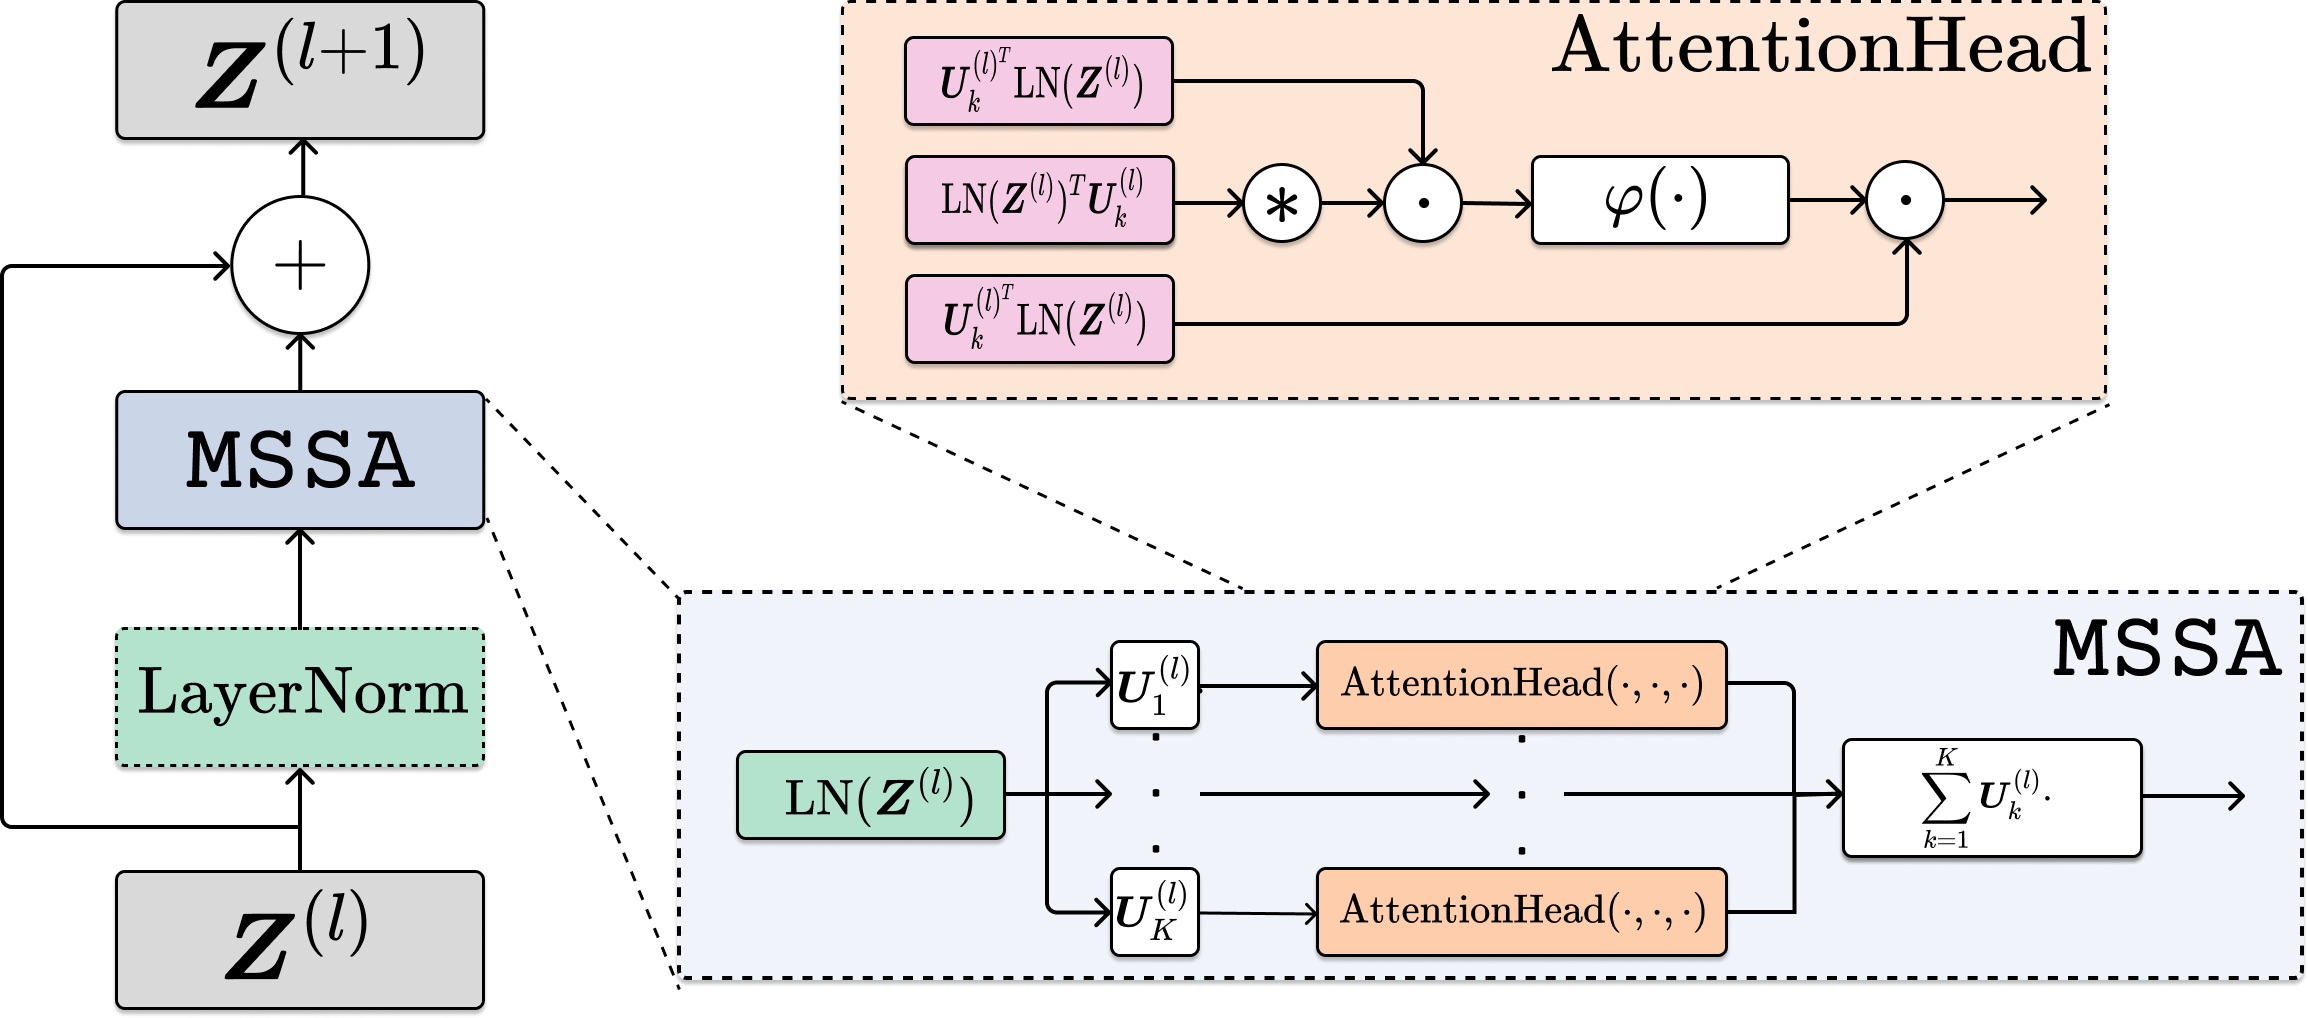
\includegraphics[width=0.75\textwidth]{\toplevelprefix/chapters/chapter4/figs/MSSA.png}
    \caption{\textbf{Detalii ale arhitecturii transformatorului doar cu atenție.} Fiecare strat constă din operatorul MSSA și o conexiune de salt. În plus, LayerNorm este inclus doar pentru sarcini de limbaj. În practică, propagarea înapoi este aplicată pentru a antrena parametrii modelului folosind eșantioane de antrenare. %
    }\label{fig:transformer}
\end{center}
\end{figure*}

\begin{theorem}\label{thm:1}
Fie $\bm Z^{(1)}$ definit în \Cref{def:MoG} și $\varphi(\cdot)$ din \eqref{eq:MSSA} să fie
$\varphi(\bm x) = h\left(\sigma(\bm x)\right)$,
unde $\sigma:\R^N \to \R^N$ este funcția softmax și $h:\R^N \to \R^N$ este o funcție de prag element cu element cu $h(x) = \tau \mathbb{I}\left\{x > \tau\right\}$ pentru fiecare $i \in [N]$. Să presupunem că $p \gtrsim \log N$, $\delta \lesssim \sqrt{\log N}/\sqrt{p}$, și
\begin{align*}
\tau \in \left( \frac{1}{2},  \frac{1}{1+N\exp(-9p/32)} \right].
\end{align*}
Pentru $N$ suficient de mare, avem cu probabilitate cel puțin $1-KLN^{-\Omega(1)}$ că pentru fiecare $\ell \in [L]$,
    \begin{align}\label{eq:SNR}
        \mathrm{SNR}(\bm Z_k^{(\ell+1)}) = (1+\eta\tau) \mathrm{SNR}(\bm Z_k^{(\ell)}),\ \forall k \in [K].
    \end{align}
\end{theorem}
Această teoremă demonstrează că atunci când reprezentările inițiale ale token-urilor sunt eșantionate dintr-un amestec de distribuții gaussiene de rang mic cu un nivel de zgomot $O(\sqrt{\log N}/\sqrt{p})$, arătăm că fiecare strat al transformatorului propus elimină zgomotul din reprezentările token-urilor la o rată liniară. Aceasta indică eficiența operatorului MSSA în reducerea zgomotului pe straturi. În mod notabil, rezultatele noastre teoretice sunt bine susținute de observațiile experimentale din \Cref{fig:MSSA}. Această teoremă oferă o fundație teoretică pentru capacitatea practică de eliminare a zgomotului a arhitecturii de transformer derivate prin desfășurarea (\ref{eq:MSSA}).

\begin{remark}
    Sub acest model, obiectivul învățării reprezentării este de a comprima un set de prezentări inițiale zgomotoase ale token-urilor în subspațiul corespunzător. Cu toate acestea, ar trebui să subliniem că în aplicațiile din lumea reală, unde reprezentările token-urilor prezintă structuri mai complicate, obiectivul învățării reprezentării este de a găsi o reprezentare compactă și structurată prin comprimarea seturilor de token-uri.
\end{remark}


\paragraph{Transformer Doar cu Atenție.} Acum, propunem formal o arhitectură de transformer doar cu atenție. Specific, prin desfășurarea pașilor de optimizare iterativă (\ref{eq:MSSA}) ca straturi ale unei rețele profunde, construim o arhitectură de transformer în \Cref{fig:transformer}. Fiecare strat al arhitecturii propuse constă doar din operatorul MSSA și o conexiune de salt. Pentru sarcini de limbaj, încorporăm suplimentar LayerNorm înainte de operatorul MSSA pentru a îmbunătăți performanța. Arhitectura completă este construită prin stivuirea unor astfel de straturi, împreună cu pași esențiali de pre-procesare și post-procesare specifici sarcinii, cum ar fi codarea pozițională, încorporarea token-urilor și capul final specific sarcinii pentru a se adapta la diferite aplicații.




În general, arhitectura standard de transformer doar-decodor este compusă din următoarele componente cheie \cite{vaswani2017attention}: (1) codare pozițională, (2) mecanisme de auto-atenție QKV multi-cap, (3) rețele MLP feed-forward, (4) normalizare pe straturi și (5) conexiuni reziduale. În contrast, arhitectura noastră de transformer propusă adoptă un design simplificat prin încorporarea mai multor simplificări cheie. Specific, folosește mecanisme de auto-atenție pe subspații cu QKV partajat, exclude straturile MLP și reduce frecvența LayerNorm.








\subsection{Atenție cu Timp Liniar: Transformer cu Statistici de Token}\label{sub:tost}

În această subsecțiune, propunem un nou operator de atenție transformer a cărui complexitate computațională scalează liniar cu numărul de token-uri pe baza obiectivului de reducere a ratei de codare. Specific, derivăm o nouă formă variațională a obiectivului MCR$^2$ și arătăm că arhitectura care rezultă din coborârea pe gradient desfășurată a acestui obiectiv variațional conduce la un nou modul de atenție numit Auto-Atenție cu Statistici de Token (\texttt{TSSA}). \texttt{TSSA} are {\em complexitate computațională și de memorie liniară} și se îndepărtează radical de arhitectura tipică de atenție care calculează similarități perechi între token-uri. Reamintim din \eqref{eq:pi} că $\bm \Pi = [\bm \pi_1, \ldots, \bm \pi_K] \in \R^{N \times K}$ denotă o matrice stocastică de „atribuire de grup" (adică, $\bm \Pi \bm 1 = \bm 1$ și $\Pi_{ik} \geq 0, \  \forall (i,k) \in [N] \times [K]$), unde $\Pi_{ik}$ denotă probabilitatea de a atribui al $i$-lea token grupului $k$.


\paragraph{O Nouă Formă Variațională pentru Ratele de Codare.} Pentru a începe, considerăm o formă generală de obiective de tip MCR$^2$ bazate pe funcții concave ale spectrului unei matrice. Și anume, pentru o matrice PSD dată $\bm M \in \PSD(d)$ și orice scalar $c \geq 0$ avem că $\log \det (\I + c \bm M) = \sum_{i=1}^{d} \log( 1 + c \lambda_i(\bm M))$, unde $\lambda_i (\bm M)$ este a $i$-a cea mai mare valoare proprie a lui $\bm M$. Mai mult, observăm că $\log(1 + c \sigma)$ este o funcție concavă necrescătoare a lui $\sigma$. Astfel, descriem rezultatele noastre în termenii unei forme mai generale de MCR$^2$ bazată pe funcții spectrale generale ale matricelor PSD de forma $F(\bm M) = \sum_{i=1}^{d} f(\lambda_i(\bm M))$, unde $f$ este concavă și necrescătoare. În particular, reamintim din discuția noastră de mai sus că mecanismul de atenție apare din desfășurarea componentei de compresie a MCR$^2$, așa că considerăm o funcție de compresie de stil MCR$^2$ mai generală:
\vspace{-2mm}
\begin{equation}
    R_{c,f}(\bm Z, \bm \Pi) \doteq \frac{1}{2}\sum_{k=1}^K \frac{N_k}{N} F\left( \frac{1}{N_k}\Z \mathrm{Diag}(\bm \pi_k) \Z^{\top} \right).
    \label{eq:mcr_c_gen}
\end{equation}



Pentru obiectivul de mai sus, observăm acum următorul rezultat:
\begin{theorem}
\label{thm:var_concave}
    Fie \(f \colon [0, \infty) \to \R\) necrescătoare, concavă și care respectă \(f(0) = 0\), și fie \(F \colon \PSD(d) \to \R\) având forma \(F(\bm M) = \sum_{i = 1}^{d}f(\lambda_{i}(\bm M))\). Atunci pentru fiecare \(\bm M \in \PSD(d)\) și \(\bm Q \in \O(d)\), avem
    \begin{equation}
        \label{eq:U_bound}
        F(\bm M) \leq  \sum_{i=1}^{d} f\left( (\bm Q^{\top} \bm M \bm Q)_{ii} \right).
    \end{equation}
    Mai mult, inegalitatea din \eqref{eq:U_bound} este atinsă cu egalitate pentru orice $\bm Q$ care diagonalizează $\bm M$, și dacă $f$ este strict concavă atunci inegalitatea din \eqref{eq:U_bound} este atinsă cu egalitate \textit{dacă și numai dacă} $\bm Q$ diagonalizează $\bm M$.
\end{theorem}

Folosind rezultatul de mai sus, putem înlocui \eqref{eq:mcr_c_gen} cu un obiectiv variațional echivalent cu forma
\vspace{-2mm}
\begin{equation}
    \label{eq:var_comp}
    R^{\rm var}_{c,f} (\Z,\bm \Pi \mid \bm U_{[K]}) \doteq \frac{1}{2}\sum_{k=1}^K \frac{N_k}{N} \sum_{i=1}^{d} f\left(\frac{1}{N_k} (\bm U_{k}^{\top} \Z \mathrm{Diag}(\bm \pi_k) \bm Z^{\top} \bm U_{k})_{ii} \right),
\end{equation}
unde echivalența este în sensul că pentru o alegere optimă a matricelor $\{ \bm U_k \in \O(d)\}_{k=1}^K$ așa cum este descris în \Cref{thm:var_concave} (adică, matrice ortogonale care diagonalizează fiecare $\Z \mathrm{Diag}(\bm \pi_k) \Z^\top $) vom atinge o limită strânsă cu $ R^{\rm var}_{c,f} (\Z,\bm \Pi \mid \bm U_{[K]}) = R_{c,f} (\Z,\bm \Pi)$. Observăm că în general, atingerea acestei limite ar necesita selectarea, pentru fiecare instanță eșantionată a lui $\Z$, a unui nou set optim de matrice parametru $\bm U_{k}$ care diagonalizează fiecare $\Z\mathrm{Diag}(\bm \pi_{k})\Z^{\top}$, ceea ce este clar impracticabil pentru arhitectura rețelei.
În schimb, ca un punct de vedere alternativ, în loc să considerăm datele ($\Z$) ca fixe și să încercăm să optimizăm parametrii $\bm U_k$ pentru a atinge limita variațională strânsă, putem în schimb să luăm principiul de design de desfășurare algoritmică descris mai sus și să proiectăm un operator pentru a perturba $\Z$ pentru a minimiza incremental $R_{c, f}^{\rm var}(\cdot \mid \bm U_{[K]})$. Pentru a face acest punct explicit, fiecare limită variațională devine strânsă când spațiile proprii ale $\Z \mathrm{Diag}(\bm \pi_k) \Z
^\top$ se aliniază cu coloanele lui $\bm U_k$, așa că prin rotirea coloanelor corespunzătoare ale lui $\Z$ (și anume, cele care corespund intrărilor mari din $\bm \pi_k$) pentru a se alinia cu $\bm U_k$ putem aborda o limită variațională strânsă. Adică, în loc să rotim $\bm U_k$ pentru a se alinia cu datele pentru fiecare instanță a lui $\Z$, putem în schimb să rotim caracteristicile token-urilor din fiecare $\Z$ pentru a se alinia cu $\bm U_k$.

Urmând această abordare, calculăm un pas de coborâre pe gradient pe $R_{c,f}^{\rm var}$ în raport cu $\Z$.
Pentru a începe acest calcul, mai întâi fie $\bm \pi \in \Re^N$ orice vector nenegativ element cu element. Atunci avem
\begin{equation}\label{eq1:grad Rcf}
\nabla_{\Z} \ \frac{1}{2} \sum_{i = 1}^{d} f(  (\Z \mathrm{Diag}(\bm \pi) \Z^{\top} )_{ii}) %
= \; \mathrm{Diag}(\nabla f[ \Z^{\hada 2} \bm \pi] ) \Z \mathrm{Diag}(\bm \pi),
\end{equation}
unde $\nabla f$ este gradientul lui $f$, și (reamintim) $\nabla f[\cdot]$ aplică $\nabla f$ la fiecare element al vectorului din paranteză. În particular, pentru $ f(x) = \log(1 + (d/\epsilon^{2}) x)$, $\nabla f(x) = (d / \epsilon^{2}) (1+ (d / \epsilon^{2}) x)^{-1}$ este pur și simplu o activare neliniară. De asemenea, (reamintim) $N_{k} = \langle \bm \pi_{k}, \bm 1\rangle$. Astfel, gradientul lui $R^{\rm var}_{c,f}$ în raport cu $\Z$ este:
\begin{align}\label{eq2:grad Rcf}
    \nabla_{\Z} R^{\rm var}_{c,f}(\Z,\bm \Pi \mid \bm U_{[K]}) =  \frac{1}{n}
    \sum_{k=1}^K \bm U_{k} \underbrace{\mathrm{Diag} \left( \nabla f\left[ (\bm
    U_{k}^{\top} \Z)^{\hada 2}  \frac{\bm \pi_k}{\langle \bm \pi_{k}, \bm 1\rangle} \right] \right)}_{\doteq \bm D(\Z, \bm \pi_{k} \mid \bm U_{k})} \bm U_{k}^{\top} \Z \mathrm{Diag}(\bm \pi_k).
\end{align}
(Observăm că constanta $1/N$ apare dintr-o constantă $(N_{k}/N)\cdot (1/N_{k}) = 1/N$ în fiecare termen al sumei.) Dacă acum considerăm un pas de gradient în raport cu al $j$-lea token $\z_j$
, ajungem la operatorul nostru de compresie incrementală propus, adică surogatorul nostru pentru un operator de \textit{auto-atenție} + rezidual:
\vspace{-2mm}
\begin{equation}\label{eq:layer-operation-orig}
    \z_j^+ = \z_{j} - \tau \nabla_{\z_{j}}R_{c, f}^{\rm var}(\Z, \bm \Pi \mid \bm U_{[K]}) = \z_j - \frac{\tau}{N} \sum_{k=1}^K \Pi_{jk} \bm U_{k} \bm D(\Z, \bm \pi_{k} \mid \bm U_{k}) \bm U_{k}^{\top} \z_j
\end{equation}
pentru fiecare \(j \in [n]\), unde $\tau > 0$ este un parametru de dimensiune a pasului pentru optimizarea incrementală. Apoi, putem construi un strat de TOST în \Cref{fig:vcrate-architecture}.

\begin{figure}[t]
    \centering 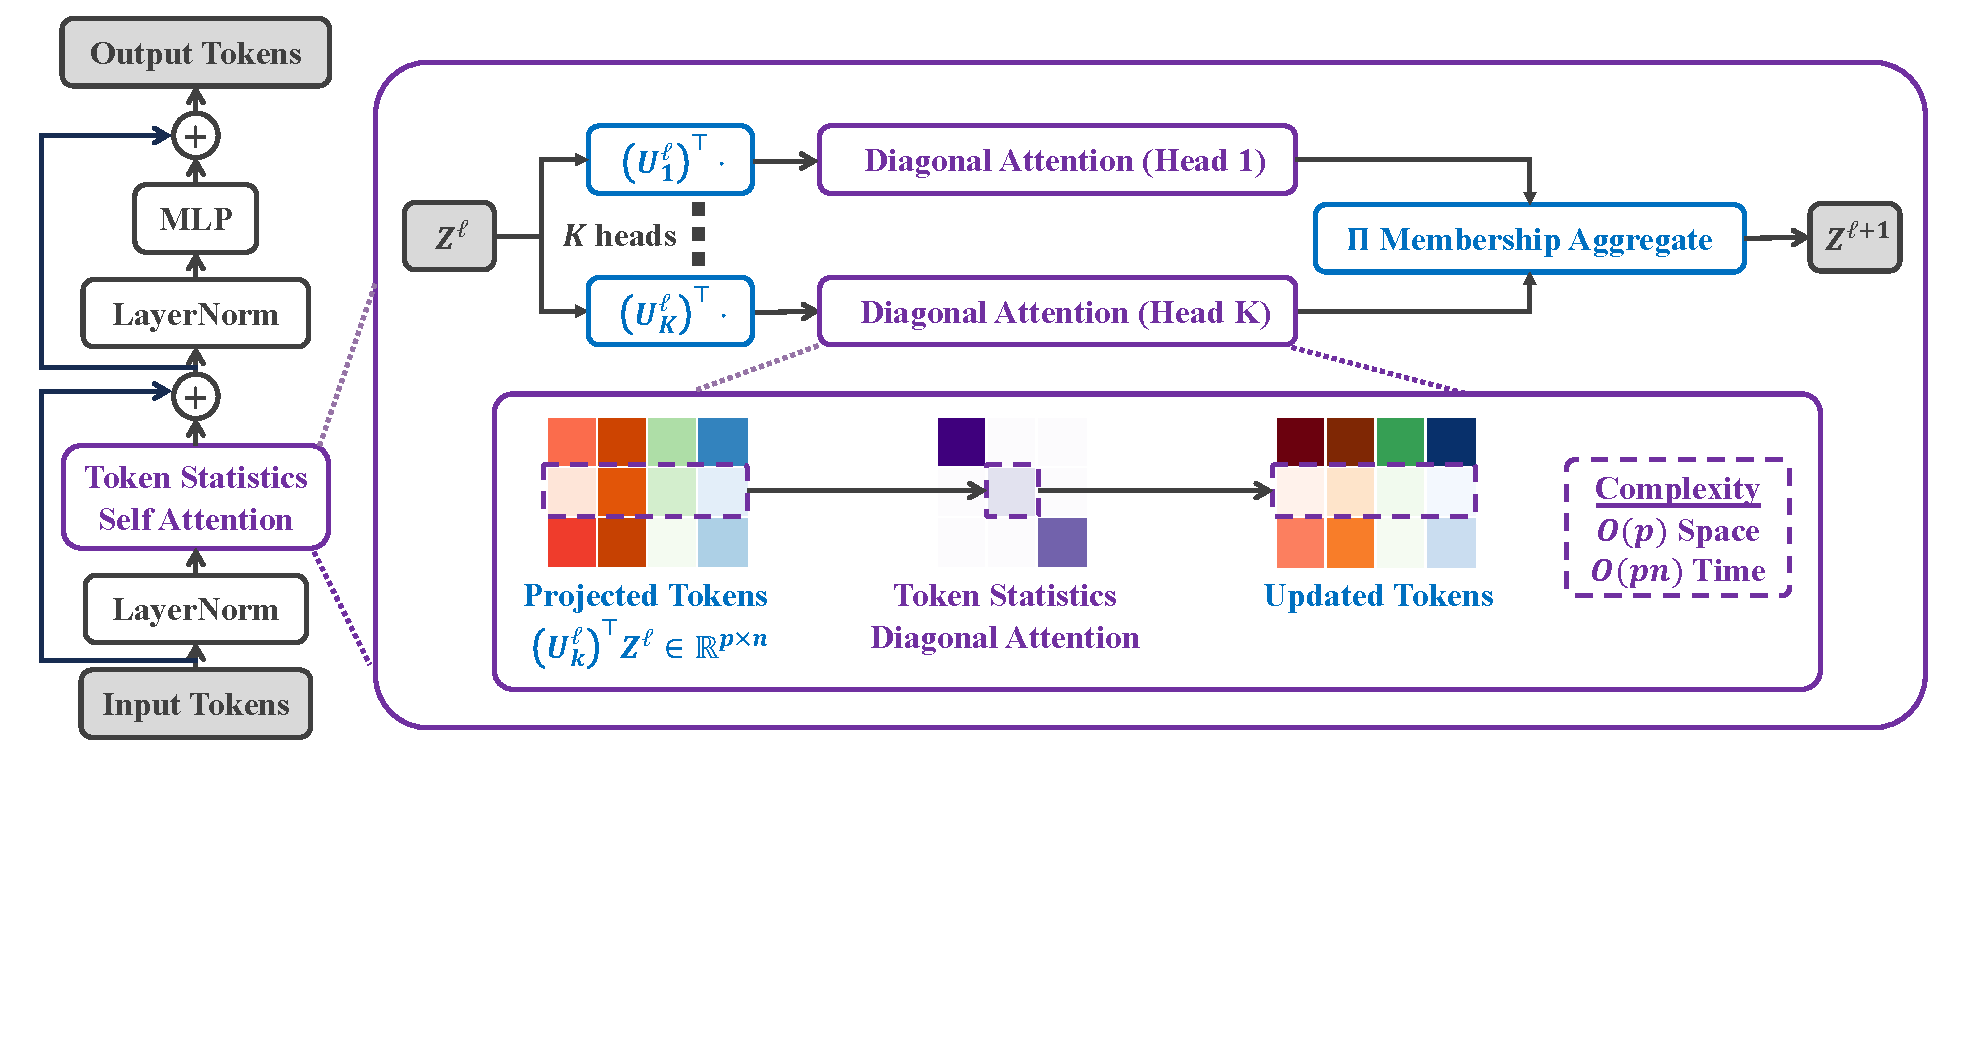
\includegraphics[width=1\textwidth,trim={0 5.0cm 0 0},clip]{\toplevelprefix/chapters/chapter4/figs/V-CRATE.pdf}
    \vspace{-1mm}
    \caption{\small \textbf{Un strat $\ell$ al Transformatorului cu Statistici de Token (ToST) propus.} În mod notabil, auto-atenția ToST transformă eficient token-urile $\Z^{\ell}$ în $\Z^{\ell+1}$, prin înmulțirea fiecărei linii a token-ului proiectat cu \textit{doar un scalar}. Aceasta conduce la complexitate redusă a atenției: are complexitate spațială $O(p)$ și complexitate temporală $O(pn)$, unde $p$ este dimensiunea token-urilor proiectate ale fiecărui cap, și $n$ este numărul de token-uri.
    }
    \label{fig:vcrate-architecture}
\end{figure}

\paragraph{Interpretarea modelului.} Dat fiind operatorul de atenție propus în \eqref{eq:layer-operation-orig}, mai întâi reamintim că liniile lui $\bm\Pi$ sunt nenegative și însumează la 1
, astfel încât operatorul nostru ia o medie ponderată a $K$ operatori de tip „cap de atenție" și apoi adaugă o conexiune reziduală. Folosind că \(\sum_{k = 1}^{K}\Pi_{jk} = 1\), putem rescrie \eqref{eq:layer-operation-orig} ca: %
\vspace{-2mm}
\begin{equation}
\label{eq:z_up}
    \z_j^+ = \sum_{k=1}^K \Pi_{jk} \Big[ \z_j \underbrace{- \frac{\tau}{n} \bm U_{k} \bm D(\Z, \bm \pi_{k} \mid \bm U_{k}) \bm U_{k}^{\top}}_{\text{acțiunea unui cap de atenție}} \z_j \Big].
\end{equation}
Adică, putem vedea fiecare cap de atenție ca mai întâi proiectând caracteristicile token-ului
pe baza $\bm U_{k}$ prin înmulțirea cu $\bm U_k^\top$, înmulțind cu
matricea diagonală $\bm D(\Z, \bm \pi_{k} \mid \bm U_{k})$ (abreviată ca \(\bm
D_{k}\)), proiectând înapoi în baza standard prin înmulțirea cu $\bm
U_{k}$, și scăzând aceasta din caracteristicile originale ale token-ului prin
conexiunea reziduală. Aspectul central al stratului nostru de atenție este calculul lui $\bm
D_{k}$. Și anume, \(\Pi_{jk} \geq 0\), astfel încât $\bm \pi_k / \langle \bm \pi_{k}, \bm
1\rangle \in \Re^N$ formează o distribuție de probabilitate asupra cărora token-uri aparțin
grupului $k$. Ca rezultat, $(\bm U^\top_k \Z)^{\hada 2} \bm \pi_k / \langle \bm \pi_{k}, \bm 1\rangle$ estimează al doilea moment al $\bm U_k^\top \Z$ sub distribuția dată de $\bm \pi_k / \langle \bm \pi_{k}, \bm 1\rangle$. Mai mult, deoarece $f$ este o funcție concavă necrescătoare, $\nabla f(x)$ descrește monoton către $0$ pe măsură ce $x$ crește, astfel încât intrările lui $\bm D_{k}$ (care au forma $\nabla f(x)$) ating maximul lor la $x=0$ %
și descresc monoton la $0$ pe măsură ce $x$ crește.

Din aceasta, ajungem la interpretarea de bază a operatorilor noștri cap de atenție + rezidual
$[\I - (\tau/n)\bm U_{k}\bm D_{k}\bm U_{k}^{\top}]$. Și anume, acest
operator face o proiecție aproximativă de rang mic dependentă de date, unde
direcțiile care au o cantitate mare de „putere" după proiecția $\bm
U_k^\top \Z$ (adică, direcții care au un al doilea moment mare $(\bm
U_{k}^{\top}\Z)^{\hada 2}\bm \pi_k / \langle \bm \pi_{k}, \bm 1\rangle$) sunt păstrate, în timp ce direcțiile care nu sunt suprimate. Pentru a vedea aceasta, reamintim că intrările lui $\bm D_k$ descresc monoton la 0 pe măsură ce al doilea moment crește, astfel încât pentru direcții cu momente secunde mari, operatorul de atenție + rezidual acționează în mare parte ca operatorul identitate. Invers, pentru direcții cu un al doilea moment mic, operatorul nostru scade o proiecție a token-urilor de-a lungul acelor direcții, rezultând în suprimarea acelor direcții. Comparativ cu operatorul standard de auto-atenție, metoda noastră în mod clar nu calculează nicio similaritate pereche între token-uri. Mai degrabă, interacțiunile dintre token-urile din $\Z$ impactează operatorul doar prin contribuția lor la statistica de al doilea moment folosită pentru a construi $\bm D_{k}$-urile. Cu toate acestea, similar cu operatorul standard de auto-atenție, metoda noastră are încă o interpretare clară ca efectuând o formă de compresie către o structură de rang mic dependentă de date, în sensul că efectuează o proiecție aproximativă de rang mic, unde direcțiile specifice care sunt suprimate sunt cele care nu sunt puternic aliniate cu alte token-uri din grup.

\paragraph{Detalii Practice de Implementare.} După ce am introdus operatorul nostru de atenție propus, discutăm acum considerații practice suplimentare. Mai întâi, până în acest punct al prezentării, am evitat discuția despre cum token-urile sunt „grupate" în diferite capete de atenție prin matricea $\bm\Pi$, dar clar este nevoie de un mijloc de construire a lui $\bm\Pi$ pentru a implementa metoda noastră. În plus, forma noastră variațională din \Cref{thm:var_concave} necesită ca matricele $\bm U$ să fie pătrate și ortogonale, dar s-ar dori în mod ideal să se folosească matrice mai mici (adică, să se reducă numărul de coloane din $\bm U$) pentru eficiență, precum și să se renunțe la constrângerile de ortogonalitate.

În practică, nu impunem constrângerile de ortogonalitate. Pentru a reduce numărul de coloane din matricele $\bm U$, observăm că similar cu CRATE \citep{yu2023white}, dacă presupunem că caracteristicile $\bm Z$ din grupul \(k\) sunt (aproximativ) grupate în jurul unui subspațiu de dimensiune mică --- să zicem de dimensiune \(p\) --- atunci covarianța în interiorul grupului-\(k\) \(\Z\mathrm{Diag}(\bm \pi_{k})\Z^{\top}\) este de rang mic, unde reamintim că \cite{yu2020learning} arată că geometria optimă a lui $\Z$ va fi ca fiecare grup să fie un subspațiu de rang mic, ortogonal pe celelalte grupuri. Putem astfel găsi explicit o bază ortonormală de dimensiune mică pentru imaginea acestei covarianțe, adică extinderea liniară a datelor din grupul \(k\). Dacă dimensiunea este $p \leq d$, baza poate fi reprezentată de o matrice ortogonală $d\times p$ $\bm U_k \in \O(d, p)$. În acest caz, putem limita superior mai eficient \(R_{c,f}\) folosind aceste matrice de bază ortogonale de rang mic. Pentru a arăta aceasta, folosim o versiune mai generală a \Cref{thm:var_concave} pentru a produce următorul corolar.
\begin{corollary}\label{cor:var_concave_logdet}
    Fie \(f \colon [0, \infty) \to \R\) necrescătoare, concavă și care respectă \(f(0) = 0\), și fie \(F \colon \PSD(p) \to \R\) având forma \(F(\bm M) = \sum_{i = 1}^{p}f(\lambda_{i}(\bm M))\). Fie \(\Z\), \(\bm \Pi\) fixe. Atunci, pentru toți \(\bm U_{1}, \dots, \bm U_{K} \in \O(d, p)\) astfel încât \(\mathrm{image}(\Z\diag(\bm \pi_{k})\Z^{\top}) \subset \mathrm{image}(\bm U_{k})\) pentru toți \(k \in [K]\), avem
    \begin{equation}
        R_{c, f}(\Z, \bm\Pi) \leq R_{c, f}^{\rm var}(\Z, \bm\Pi \mid \bm U_{[K]}), 
    \end{equation}
     unde \(R_{c, f}^{\rm var}\) este definit formal în \eqref{eq:var_comp}. Egalitatea este valabilă dacă \(\bm U_{k}\) diagonalizează \(\Z\diag(\bm \pi_{k})\Z^{\top}\) pentru fiecare \(k \in [K]\), și dacă \(f\) este puternic concavă atunci această condiție de egalitate devine un „dacă și numai dacă."
\end{corollary}

Pasul final pentru a defini operatorul nostru de atenție este să estimăm apartenența la grup $\bm\Pi$. Pentru aceasta postulăm un model simplu despre cum fiecare caracteristică \(\z_{j}\) deviază de la subspațiul său suport și apoi găsim atribuirea optimă de subspațiu. \cite{yu2023white} arată că dacă modelăm independent fiecare \(\z_{j}\) ca aparținând unui model de amestec gaussian de dimensiune mică, unde fiecare gaussiană are o matrice de covarianță cu spectru identic și este susținută pe un subspațiu cu bază ortonormală \(\bm U_{k}\), plus zgomot gaussian independent cu covarianță \(\eta \I\), atunci probabilitatea posterioară că fiecare token \(\z_{j}\) aparține fiecărui subspațiu este dată de matricea de atribuire \(\bm \Pi = \bm \Pi(\bm Z \mid \bm U_{[K]})\) după cum urmează:
\begin{align}\label{eq:pi}
    \bm \Pi = \begin{bmatrix} \boldsymbol{\nu}(\z_1 \mid \bm U_{[K]})^\top \\ \vdots \\ \boldsymbol{\nu}(\z_n \mid \bm U_{[K]})^\top \end{bmatrix}, \quad
\text{unde} \quad 
\boldsymbol{\nu}(\z_j \mid \bm U_{[K]}) \doteq \operatorname{softmax}\left( \frac{1}{2\eta} \begin{bmatrix} \|  \bm U_{1}^{\top} \z_j \|_2^2 \\ \vdots \\ \| \bm U_{K}^{\top} \z_j \|_2^2 \end{bmatrix} \right), \quad \forall j \in [n],
\end{align}
unde $\eta$ devine un parametru de temperatură învățabil. Astfel, dată fiind o caracteristică de intrare \(\Z\), estimăm \(\bm\Pi\) folosind \eqref{eq:pi} și apoi calculăm operatorul de atenție. Combinând construcția lui $\bm\Pi$ din \eqref{eq:pi} cu
\eqref{eq:layer-operation-orig}, obținem operatorul {\em Auto-Atenție cu Statistici de Token}:
\begin{equation}
    \label{eq:tssa}
   \texttt{TSSA}(\Z \mid \bm U_{[K]}) \doteq -\frac{\tau}{n}\sum_{k = 1}^{K}\bm U_{k}\bm D(\Z, \bm\pi_{k} \mid \bm U_{k})\bm U_{k}^{\top}\Z\diag(\bm \pi_{k}),
\end{equation}
unde \(\bm\pi_{k}\) sunt coloanele lui \(\bm\Pi = \bm\Pi(\Z \mid \bm U_{[K]})\) definit în \eqref{eq:pi} și \(\bm D\) este definit în \eqref{eq2:grad Rcf}.




\section{Rezumat și Note}




Materialele prezentate în acest capitol se bazează pe o serie de lucrări recente pe această temă, inclusiv \cite{chan2021redunet, wang2024global, wang2025attention, wu2025token, yu2023white}. Aceste contribuții cuprind atât progrese teoretice, cât și metodologii practice pentru construirea rețelelor profunde interpretabile prin optimizare desfășurată. Multe dintre rezultatele și demonstrațiile cheie discutate în acest capitol sunt derivate direct din, sau inspirate de, aceste lucrări fundamentale.


Ideea de a desfășura un algoritm de optimizare pentru a construi o rețea neuronală datează de la lucrarea seminală \cite{gregor2010learning}. În această lucrare, autorii au demonstrat că algoritmii de codare rară—cum ar fi Algoritmul de Prag de Micșorare Iterativă (ISTA)—pot fi desfășurați pentru a forma perceptroni multistrat (MLP-uri), făcând efectiv legătura între optimizarea iterativă și designul rețelelor neuronale. În mod notabil, \cite{monga2019algorithm} a demonstrat că astfel de rețele desfășurate sunt mai interpretabile, mai eficiente din punct de vedere al parametrilor și mai eficace comparativ cu rețelele generice. În acest capitol, ne bazăm pe această perspectivă pentru a dezvolta arhitecturi de rețele profunde cu cutie albă principiale prin desfășurarea algoritmilor de optimizare care sunt proiectați să minimizeze obiective bine motivate—cum ar fi obiectivul de reducere a ratei (rare) introdus anterior. Această abordare nu numai că clarifică rolul fiecărui strat din rețea, dar oferă și o fundamentare teoretică pentru alegerile arhitecturale, depășind încercarea și eroarea empirică către un design interpretabil și orientat spre obiective. În continuare, comparăm DNN-urile convenționale, care sunt de obicei construite prin design empiric și ajustare euristică, cu arhitecturile noastre ReduNet fundamentate matematic:

\begin{center}
\begin{tabular}{| l || c | c |}
\hline
  & DNN-uri Convenționale & ReduNets\\ [0.5ex]
  \hline \hline
Obiective & potrivire intrare/ieșire & câștig de informație\\ [0.5ex]
  \hline
Arhitecturi profunde & încercare și eroare & optimizare iterativă \\  [0.5ex]
\hline
Operatori de strat & empirici & gradient proiectat \\  [0.5ex]
\hline
Invarianță la deplasare & CNN-uri+augmentare & ReduNets invariante \\  [0.5ex]
\hline
Inițializări & aleatorii/pre-proiectate & desfășurate înainte \\ [0.5ex]
\hline
Antrenare/ajustare fină & propagare înapoi & propagare înainte/înapoi\\ [0.5ex]
\hline
Interpretabilitate & cutie neagră & cutie albă \\ [0.5ex]
\hline
Reprezentări & ascunse/latente & subspații incoerente \\ [0.5ex]
\hline
\end{tabular}
\end{center}




\section{Exerciții și Extensii}


\begin{exercise}
    Fie $\bm Z = [\bm Z_1,\dots,\bm Z_K] \in \R^{d\times m}$ cu $\bm Z_k \in \R^{d\times m_k}$ pentru fiecare $k \in [K]$. Pentru un anumit $\alpha > 0$, fie
    \begin{align*}
        R(\bm Z) = \log\det\left(\bm I + \alpha\bm Z\bm Z^T \right).
    \end{align*}
1. Dată fiind orice direcție $\bm D \in \R^{d\times m}$, vă rugăm să arătați că $\nabla R(\bm Z) = \alpha\bm X^{-1}\bm Z$ și
    \begin{align*}
 \nabla^2 R(\bm Z)[\bm D, \bm D] =\alpha \mathrm{Tr}\left( \bm X^{-1}\bm D\bm D^T\right) - \frac{\alpha^2}{2}\mathrm{Tr}\left(\bm X^{-1}\left( \bm Z\bm D^T+\bm D\bm Z^T\right) \bm X^{-1}\left( \bm Z\bm D^T+\bm D\bm Z^T\right)\right),
    \end{align*}
    unde $\bm X \doteq \bm I + \alpha\bm Z\bm Z^T$. {\em Indiciu:} Observați că
    \begin{align*}
        \nabla^2 R(\bm Z)[\bm D, \bm D] \doteq \left\langle \lim_{t \to 0} \frac{\nabla R(\bm Z+ t\bm D) - \nabla R(\bm Z)}{t}, \bm D \right\rangle. 
    \end{align*}

\noindent
2. Vă rugăm să arătați că
\begin{align*}
    R(\bm Z) \le \sum_{k=1}^K \log\det\left(\bm I + \alpha\bm Z_k\bm Z_k^T \right),
\end{align*}
unde egalitatea este valabilă dacă și numai dacă $\bm Z_k^T\bm Z_l = \bm 0$ pentru toți $k \neq l \in [K]$.
\medskip 

\noindent 
3. Dat fiind un anumit $\alpha >0$, fie $\alpha_k=m\alpha/m_k$ pentru fiecare $k \in [K]$. Vă rugăm să derivați forma închisă pentru punctul critic de ordinul întâi al următoarei funcții:
\begin{align*}
    f(\bm Z_k) = \frac{1}{2}\log\det\left(\bm I + \alpha\bm Z_k\bm Z_k^T \right) - \frac{m_k}{2m}\log\det\left(\bm I + \alpha_k \bm Z_k\bm Z_k^T \right) - \frac{\lambda}{2}\|\bm Z_k\|_F^2. 
\end{align*}
{\em Indiciu:} Fie $r_k=\mathrm{rank}(\bm Z_k)$. Considerați următoarea descompunere în valori singulare a lui $\bm Z_k$:
\begin{align*}
    \bm Z_k = \bm P_k\bm \Sigma_k\bm Q_k^T = \begin{bmatrix}
        \bm P_{k,1} & \bm P_{k,2}
    \end{bmatrix} \begin{bmatrix}
        \tilde{\bm \Sigma}_{k} & \bm 0 \\
        \bm 0 & \bm 0
    \end{bmatrix} 
    \begin{bmatrix}
        \bm Q_{k,1}^T \\ \bm Q_{k,2}^T
    \end{bmatrix}, 
\end{align*}
unde $\bm P_k \in \mathcal{O}^d$ cu $\bm P_{k,1} \in \R^{d\times r_k}$ și $\bm P_{k,2} \in \R^{d\times (d-r_k)}$, $\bm \Sigma_k \in \R^{d\times m_k}$ cu $\tilde{\bm \Sigma}_{k} \in \R^{r_k\times r_k}$ fiind o matrice diagonală, și $\bm Q_k \in \mathcal{O}^{m_k}$ cu $\bm Q_{k,1} \in \R^{m_k\times r_k}$ și $\bm P_{k,2} \in \R^{m_k \times (m_k-r_k)}$.
\medskip 

\end{exercise}


\begin{exercise}[Seria Neumann pentru inversa matricei]\label{ex:neumannn}
Fie $\bm A \in \mathbb{R}^{n\times n}$. Dacă $\|\bm A\| < 1$, vă rugăm să arătați
\begin{align}\label{eq:neumann}
    \left( \bm I - \bm A\right)^{-1} = \sum_{k=1}^\infty \bm A^k.  
\end{align}
{\em Indiciu:} Demonstrația constă din doi pași. \\
(i) {\bf Pasul 1}: Vă rugăm să arătați că seria infinită $\sum_{k=1}^\infty \bm A^k$ converge când $\bm A < 1$ folosind $\|\bm A^k\| \le \|\bm A\|^k$. \\
(ii) {\bf Pasul 2}: Calculați produsul matriceal $(\bm I - \bm A) \sum_{k=1}^\infty \bm A^k$.
\end{exercise}


\begin{exercise}
    Vă rugăm să calculați gradienții din \eqref{eq1:grad Rcf} și \eqref{eq2:grad Rcf}.
\end{exercise}


\begin{exercise}
    Vă rugăm să arătați \Cref{cor:var_concave_logdet} când $Kp \le d$.
\end{exercise}

\end{document>